\documentclass[12pt,a4paper]{article}
\usepackage[utf8]{inputenc}

\usepackage{amsmath}
\usepackage{amsfonts}
\usepackage{amssymb}
\usepackage{graphicx}
\usepackage{listings}
\usepackage[margin=1.0in]{geometry}
\usepackage{caption}
\usepackage{subcaption}
\usepackage{float}
\usepackage[utf8]{inputenc}
\usepackage{refstyle}
\usepackage{spverbatim}
\usepackage{listings}
\usepackage{csvsimple}
\usepackage{adjustbox}
\usepackage{cancel}
\usepackage{scalerel,stackengine}
\stackMath
\newcommand\reallywidehat[1]{%
\savestack{\tmpbox}{\stretchto{%
  \scaleto{%
    \scalerel*[\widthof{\ensuremath{#1}}]{\kern-.6pt\bigwedge\kern-.6pt}%
    {\rule[-\textheight/2]{1ex}{\textheight}}%WIDTH-LIMITED BIG WEDGE
  }{\textheight}% 
}{0.5ex}}%
\stackon[1pt]{#1}{\tmpbox}%
}
\parskip 1ex

\lstset{numbers=left,
	title=\lstname,
	numberstyle=\tiny, 
	breaklines=true,
	tabsize=4,
	language=Python,
	morekeywords={with,super,as},,
	frame=single,
	basicstyle=\footnotesize\tt,
	commentstyle=\color{comment},
	keywordstyle=\color{keyword},
	stringstyle=\color{string},
	backgroundcolor=\color{background},
	showstringspaces=false,
	numbers=left,
	numbersep=5pt,
	literate=
		{æ}{{\ae}}1
		{å}{{\aa}}1
		{ø}{{\o}}1
		{Æ}{{\AE}}1
		{Å}{{\AA}}1
		{Ø}{{\O}}1
	}

\usepackage{bm}
\usepackage{hyperref}
\usepackage[usenames, dvipsnames]{color}

\begin{document}

\begin{center}
\LARGE{\textbf{Project 1}}
\\
\large{\textbf{Course: FYS-STK4155}}
\\
\large{\textbf{Semester: Autumn 2020}}
\\
\large{\textbf{Name: Sander Losnedahl}}
\end{center}


\newpage

\begin{center}
\Large{\textbf{Preliminaries}}
\end{center}

\noindent This report will cover a few important, but necessary steps in the regression scheme before presenting the results form the sub-exercises. Each of these steps are implemented in all the exercises and will ultimately yield a more reliable result.
\\
\textbf{Scaling the data} is necessary in order to make sense of the output values. If the data is unscaled, the resulting numbers will not make much sense as we have no reference to what are low and high numbers. When we scale the data we subtract the sample mean and divide by the sample standard deviation of the data, we essentially make the data centred around zero with standard deviation one. This way, we always have a reference to the outcome as it is always relative to zero. Additionally, most regression algorithms rely on the data having lower distance between the data points, making scaling an important pre-processing step.
\\
\textbf{The number of observations n} has large impact on the regression algorithm and the results from it. Typically, having more data (larger n) results in a better estimation of the response. In fact, some algorithms like ordinary least squares rely on the number of observations to be greater than the polynomial degree p of the design matrix. Moreover, algorithms like ordinary least squares work best when $n >> p$. In this project, we will initially experiment with different sizes of n, but later exercises will use $n = 100$.
\\
\textbf{Noise level} is a recurrent theme throughout this report. Noise is added to the design matrix itself (sub exercise a-e) in order to prepare for the real data. The noise that is added has a standard normal distribution with standard deviation $1$ and maximum value of $1$ at its mean of zero. This noise is then multiplied with a constant of $0.001$ in order to adjust the noise level. 
\\
\textbf{The train/test split} will be $75/25$ in this project. When performing regression, we need to both train the algorithm using the training set, and later validate the trained algorithm using the independent test set. There is no set ratio which is considered the best, but the training set should include the majority of the observations n. 

\newpage

\begin{center}
\Large{\textbf{Exercise 1.}}
\end{center}

\noindent \textbf{a)} The goal for this part of the exercise is trying to fit a linear model (linear in terms of regression coefficients) to the Franke function given as

\begin{equation}\label{eq:Franke}
\begin{aligned}
f(x,y) &= \frac{3}{4}\exp{\left(-\frac{(9x-2)^2}{4} - \frac{(9y-2)^2}{4}\right)}+\frac{3}{4}\exp{\left(-\frac{(9x+1)^2}{49}- \frac{(9y+1)}{10}\right)} \\
&+\frac{1}{2}\exp{\left(-\frac{(9x-7)^2}{4} - \frac{(9y-3)^2}{4}\right)} -\frac{1}{5}\exp{\left(-(9x-4)^2 - (9y-7)^2\right) }
\end{aligned}
\end{equation}

\noindent where polynomial combinations of x and y in the span $x,y \in [0,1]$ will be the explanatory variables. The linear regression equation then takes the form

\begin{equation}\label{eq:LinReg}
\begin{aligned}
\reallywidehat{f(x,y)} = \hat{y} = \textbf{X} \boldsymbol{\beta + \epsilon}
\end{aligned}
\end{equation}

\noindent where $\reallywidehat{f(x,y)}$ or $\hat{y}$ is the least squares estimate of the Franke function, $\textbf{X}$ is the $n\times p$ design matrix consisting of the aforementioned polynomial combinations of x and y, $\boldsymbol{\beta}$ are the $p\times 1$ regression coefficients and $\boldsymbol{\epsilon}$ is just random noise/unobserved random variables. In order to get the best estimate for the Franke function, we want to choose $\boldsymbol{\beta}$-values so that we minimize the residual sum of squares (thereby the name "least squares"). Solving equation \ref{eq:LinReg} with the intent to minimize the residual sum of squares yields the estimates for the $\boldsymbol{\beta}$-values 

\begin{equation}\label{eq:minBeta}
\begin{aligned}
\hat{\boldsymbol{\beta}} = (\textbf{X}^T\textbf{X})^{-1}\textbf{X}^T f(x,y)
\end{aligned}
\end{equation}

\noindent where T marks the transpose of the matrix. We can now get the estimate $\hat{\boldsymbol{\beta}}$ with equation \ref{eq:minBeta} and then compute the estimate of the Franke function as seen in equation \ref{eq:LinReg}.
\\
We now turn to implementing the regression algorithm (see github) where we start by selecting a low number of observations of $n = 10$, a polynomial degree of $p = 5$ and a noise level of $0.001$. We start by creating the design matrix using polynomials of x and y (and their combinations) of degrees up to 5, scale it, split it into training and test set with ratio $75/25$ and lastly estimate the regression coefficients and calculate the estimated Franke function. The regression coefficients are then found, but it is not always certain which values of beta coefficients minimize the residual sum of squares, so some uncertainty is always present. Therefore, we need to find which coefficients are uncertain, and which are certain. We quantify the uncertainty by using confidence intervals around the coefficients such that our uncertainty is within one standard deviation of the coefficient. We find said standard deviation by taking the square root of the diagonal elements of the covariance matrix 

\begin{equation}\label{eq:diagCOV}
\begin{aligned}
\sigma = \sqrt{diag((\textbf{X}^T\textbf{X})^{-1}S^2)}
\end{aligned}
\end{equation}

\noindent where X is the design matrix and S is the sample variance of the response. By then taking $\beta_i \pm \sigma_i$ we can find the confidence interval of the regression coefficients which is plotted in figure \ref{fig:betaIntALL1}

\begin{figure}[H]
\centering
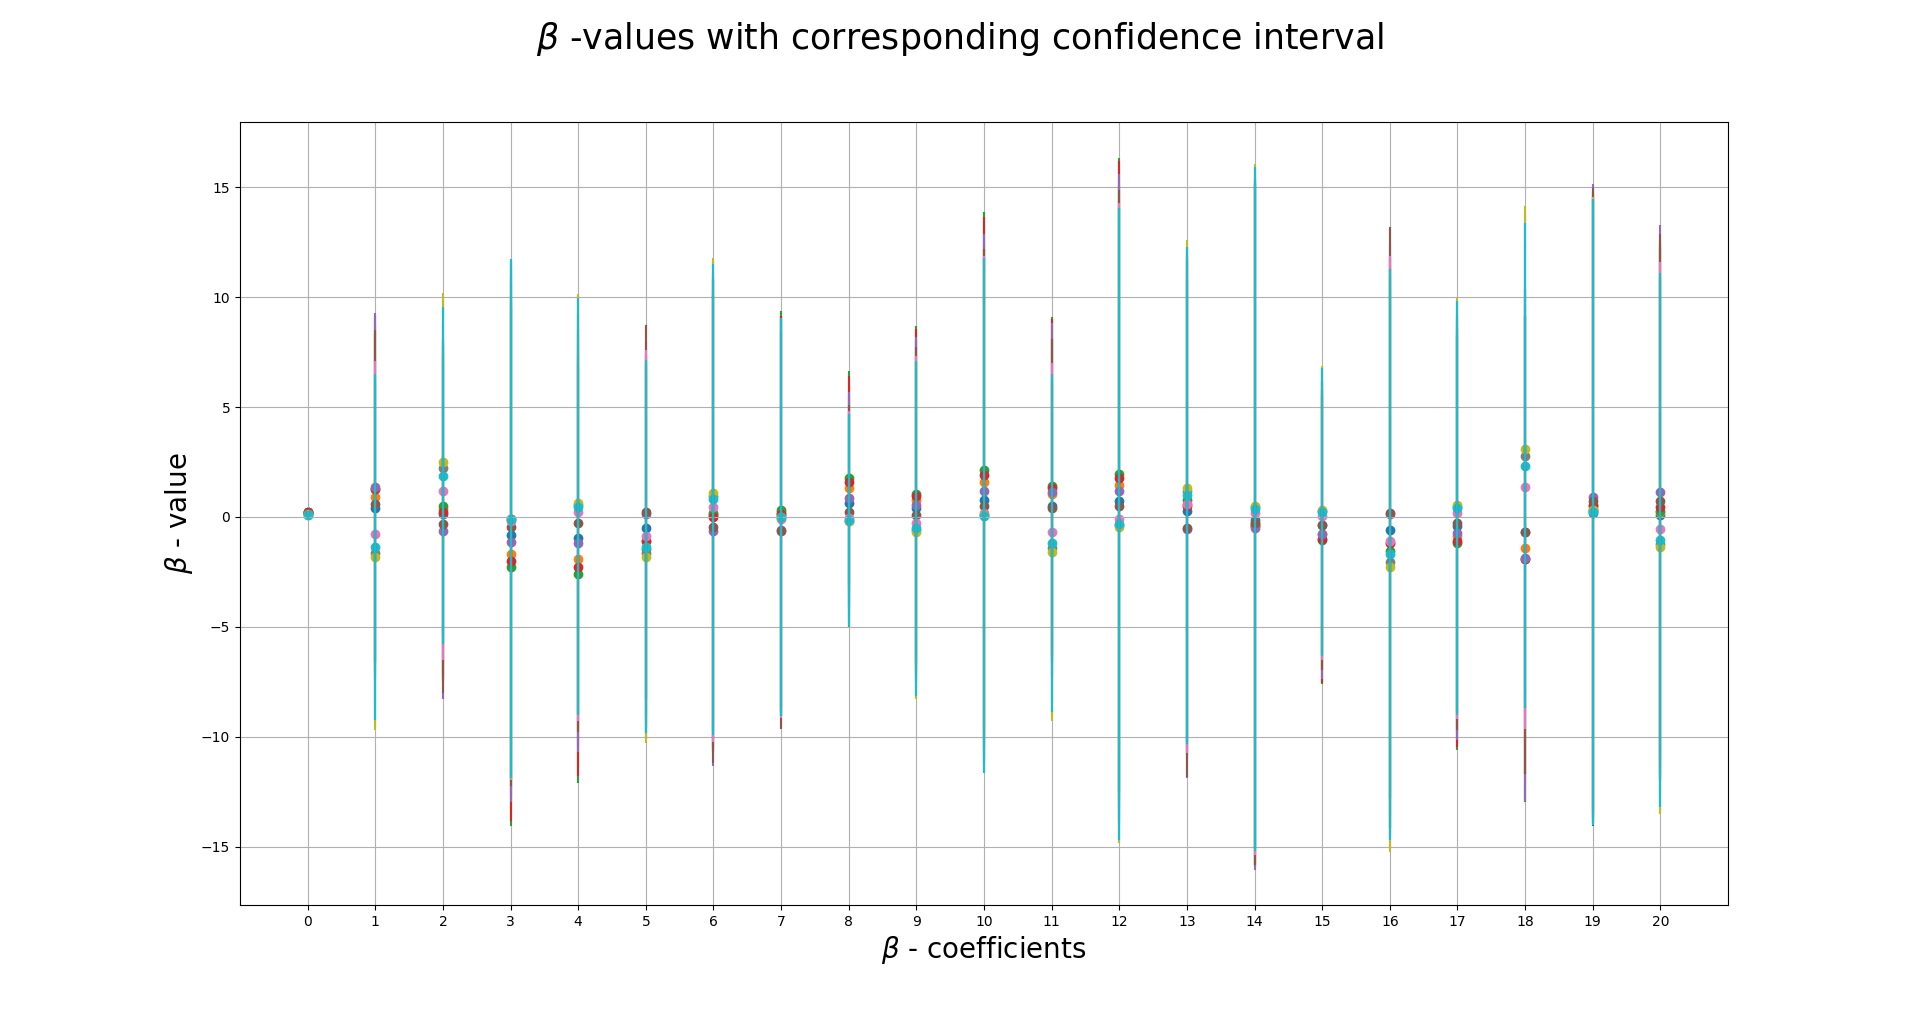
\includegraphics[width = 1\linewidth]{C:/Users/Sander/Documents/GitHub/FYS-STK4155/Project1/Report/Figures/betaInterval_ALL_n10_p5_noise0001_ts025.PNG}
\caption{\label{fig:betaIntALL1} $\hat{\boldsymbol{\beta}}$-coefficients from performing ordinary least squares regression. Dots indicate the actual $\hat{\boldsymbol{\beta}}$-coefficients value while bars around indicate the confidence interval ($\pm \sigma$).}
\end{figure}

\noindent Since the response is the Franke function (a matrix), we get p times n regression coefficients instead of p, as seen in figure \ref{fig:betaIntALL1}. However, one can still observe from figure \ref{fig:betaIntALL1} that some regression coefficients are more certain than others. We can also plot one slice of the p times n regression coefficient matrix to get a better view as seen in figure \ref{fig:betaIntROW1}

\begin{figure}[H]
\centering
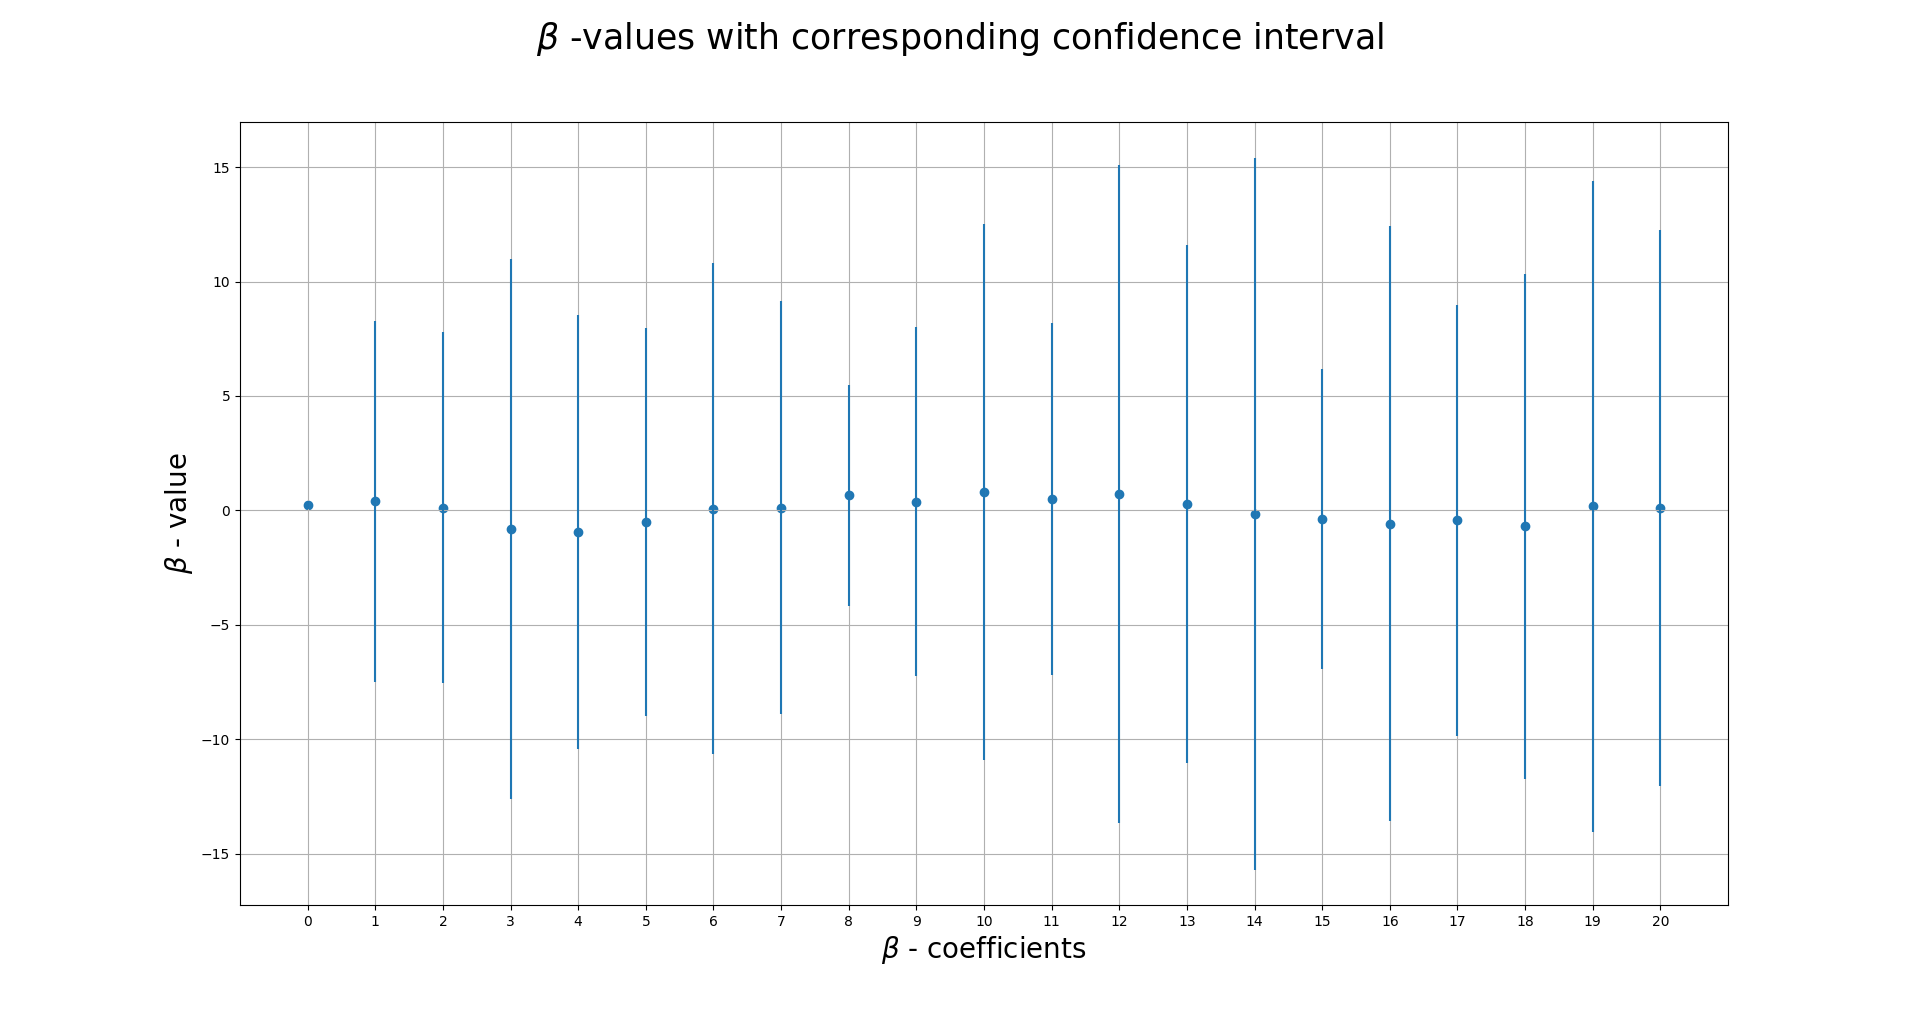
\includegraphics[width = 1\linewidth]{C:/Users/Sander/Documents/GitHub/FYS-STK4155/Project1/Report/Figures/betaInterval_1row_n10_p5_noise0001_ts025.PNG}
\caption{\label{fig:betaIntROW1} A slice of the $\hat{\boldsymbol{\beta}}$-coefficients from performing ordinary least squares regression. Dots indicate the actual $\hat{\boldsymbol{\beta}}$-coefficients value while bars around indicate the $95\%$ confidence interval ($\pm \sigma$).}
\end{figure}

\noindent Now that we have calculated and gained some faith in our regression coefficient estimates, we can utilize equation \ref{eq:LinReg} to find $\hat{y}$ which is plotted together with the real Franke function in figures \ref{fig:FrankeReal1} and \ref{fig:FrankeEst1}

\begin{figure}[H]
\centering
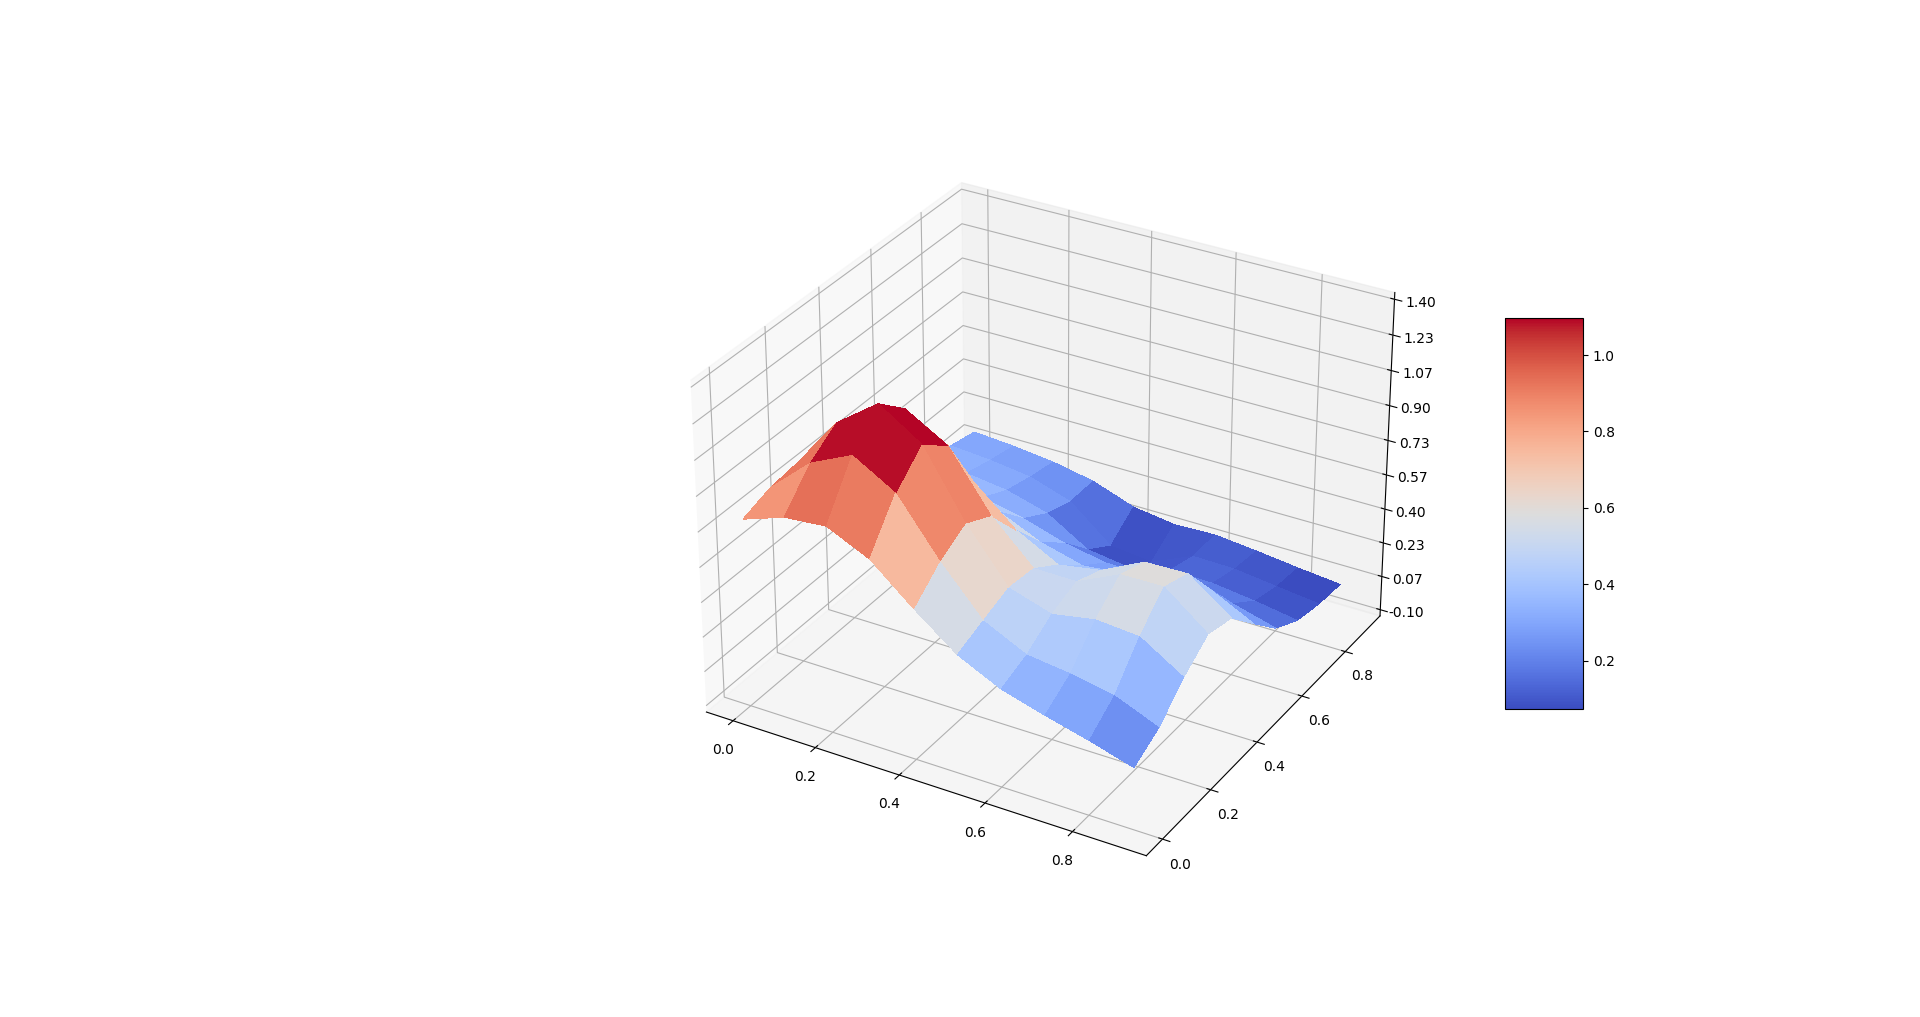
\includegraphics[width = 1\linewidth]{C:/Users/Sander/Documents/GitHub/FYS-STK4155/Project1/Report/Figures/zReal_n10_p5_noise0001_ts025.PNG}
\caption{\label{fig:FrankeReal1} The real Franke function when we have $10$ observations and polynomials of degree $5$ using a noise-level of $0.001$ and a $75/25$ train/test split.}
\end{figure}

\begin{figure}[H]
\centering
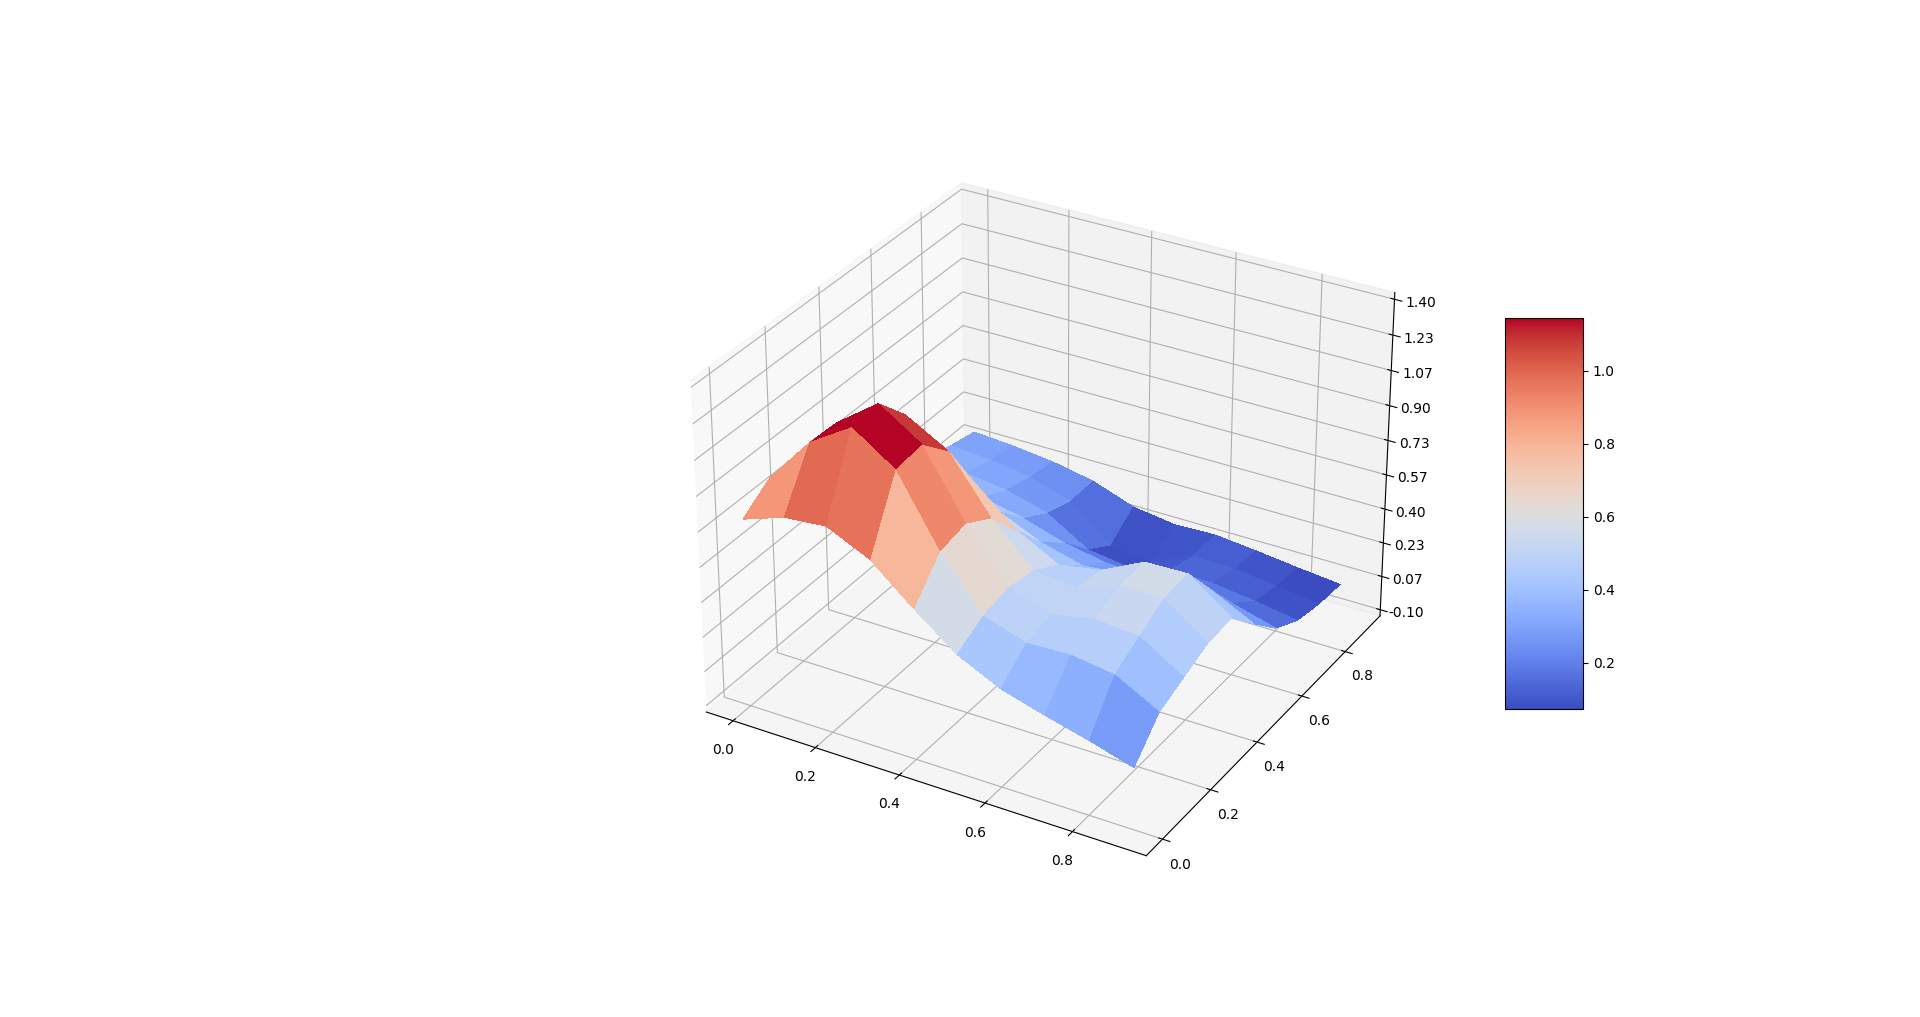
\includegraphics[width = 1\linewidth]{C:/Users/Sander/Documents/GitHub/FYS-STK4155/Project1/Report/Figures/zEst_n10_p5_noise0001_ts025.PNG}
\caption{\label{fig:FrankeEst1} The estimated Franke function when we have $10$ observations and polynomials of degree $5$ using a noise-level of $0.001$ and a $75/25$ train/test split.}
\end{figure}

\noindent It can be observed from figures \ref{fig:FrankeReal1} and \ref{fig:FrankeEst1} that our estimate is pretty good, any we can plot the difference between the two to strengthen faith in the model

\begin{figure}[H]
\centering
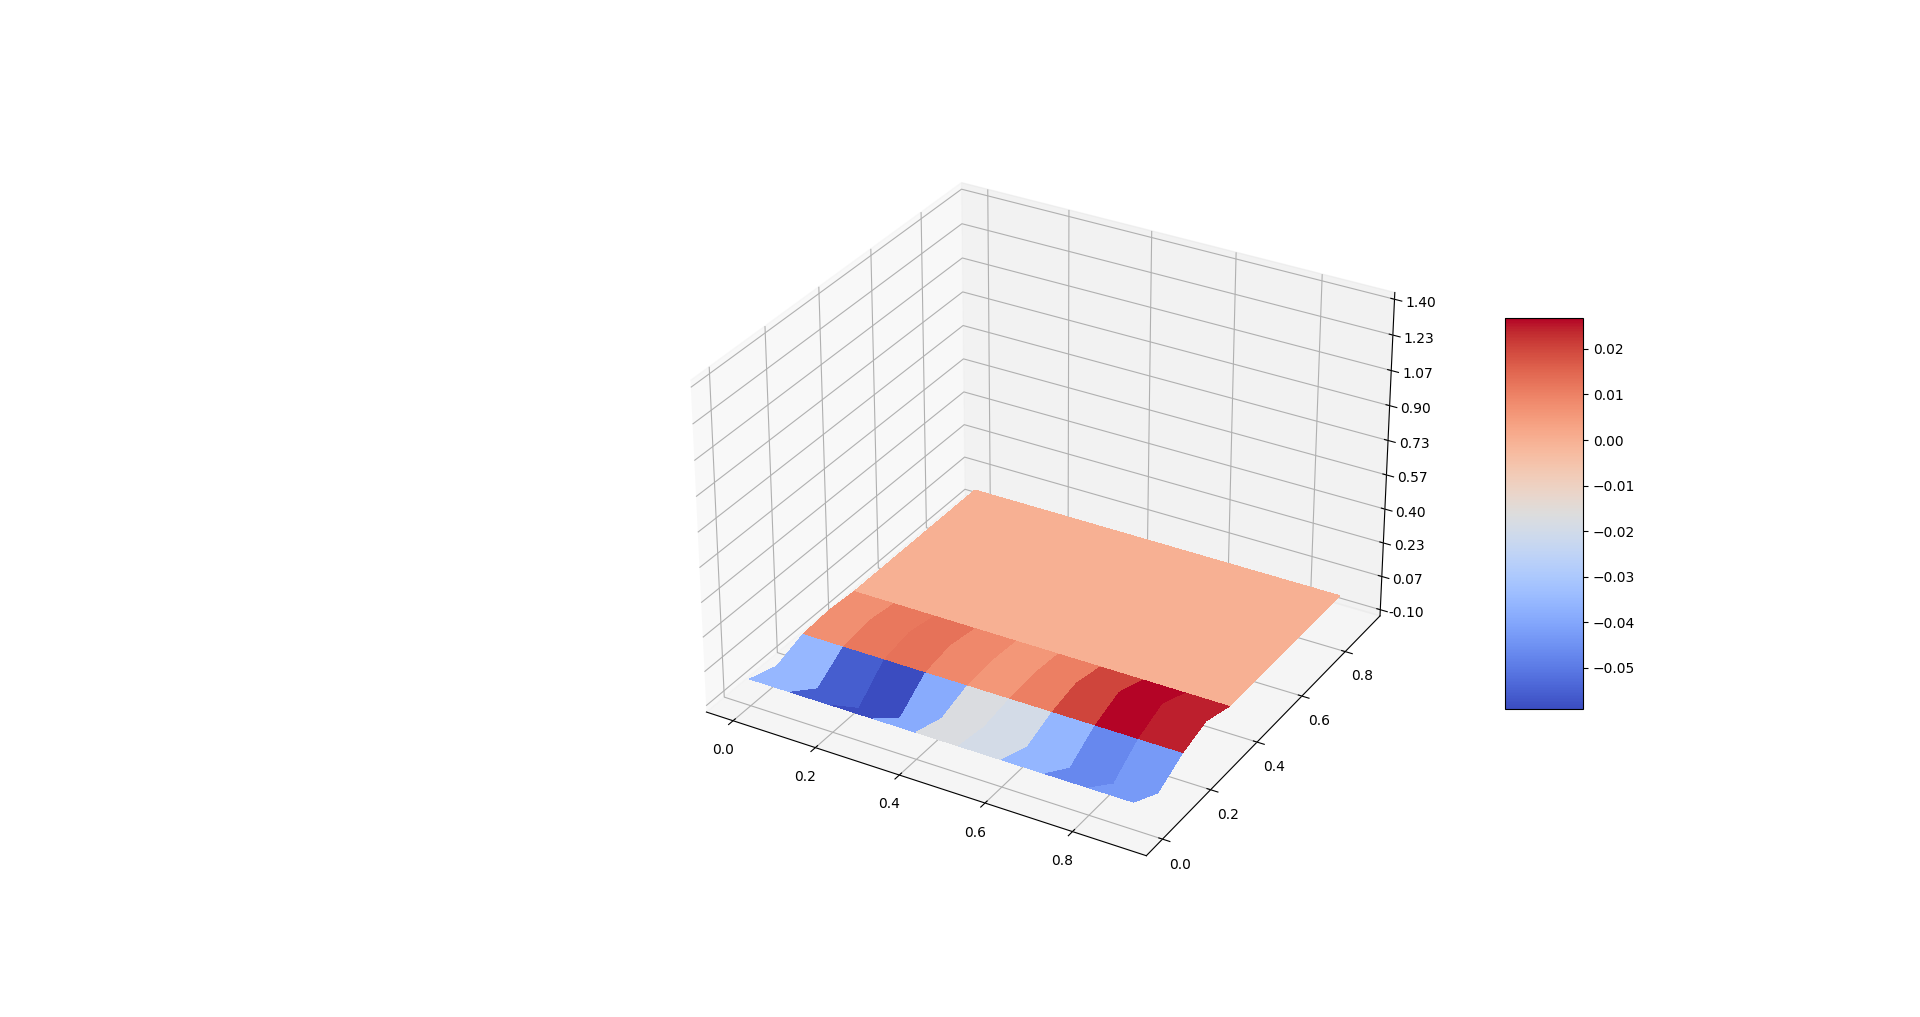
\includegraphics[width = 1\linewidth]{C:/Users/Sander/Documents/GitHub/FYS-STK4155/Project1/Report/Figures/zDiff_n10_p5_noise0001_ts025.PNG}
\caption{\label{fig:FrankeDIFF1} The difference between the real and estimated Franke functions when we have $10$ observations and polynomials of degree $5$ using a noise-level of $0.001$ and a $75/25$ train/test split.}
\end{figure}

\noindent As expected, the difference shown in figure \ref{fig:FrankeDIFF1} is very small. However, we have yet to quantify how small. This can be done using the mean square error (MSE) and $R^2$ which is calculated from equations \ref{eq:MSE} and \ref{eq:R2}

\begin{equation}\label{eq:MSE}
\begin{aligned}
MSE = \frac{1}{n} \sum_{i=0}^{n-1}(y_i-\hat{y}_i)^2
\end{aligned}
\end{equation}

\begin{equation}\label{eq:R2}
\begin{aligned}
R^2 = 1- \frac{\sum_{i=0}^{n-1}(y_i-\hat{y}_i)^2}{\sum_{i=0}^{n-1}(y_i-\bar{y}_i)^2}
\end{aligned}
\end{equation}

\noindent where $\bar{y}_i$ is the mean value of the Franke function. The MSE gives us a value of how far our estimate falls from the real Franke function, while the $R^2$ gives us how strong the relationship is between the real Franke function and our estimate. When utilizing equations \ref{eq:MSE} and\ref{eq:R2} on the data shown in figures \ref{fig:FrankeReal1} and \ref{fig:FrankeEst1} we get the values in table \ref{tab:ESTREAL1}

\begin{table}[h]
\caption{\label{tab:ESTREAL1} MSE and $R^2$ between the real and estimated Franke function when we have $10$ observations and polynomials of degree $5$ using a noise-level of $0.001$ and a $75/25$ train/test split.}
\centering
\begin{tabular}{c|c|c}
 & MSE & $R^2$\\
\hline
Training & $2.4978127439196968 \times 10^{-24}$ & $1.0$\\
\hline
Test & $0.003919934844588911$ & $0.9425989967371673$\\	  
\end{tabular}
\end{table}

\noindent It should be obvious that the training set performs better than the test, as it is the training data that is used to fit the model, particularly when n is small. So what happens when we increase the number of observations to say $n = 100$? Figures QQQ, QQQ and QQQ show again the real, estimated and differential Franke functions with the same exact parameters, except for n, which is now equal to $100$

\begin{figure}[H]
\centering
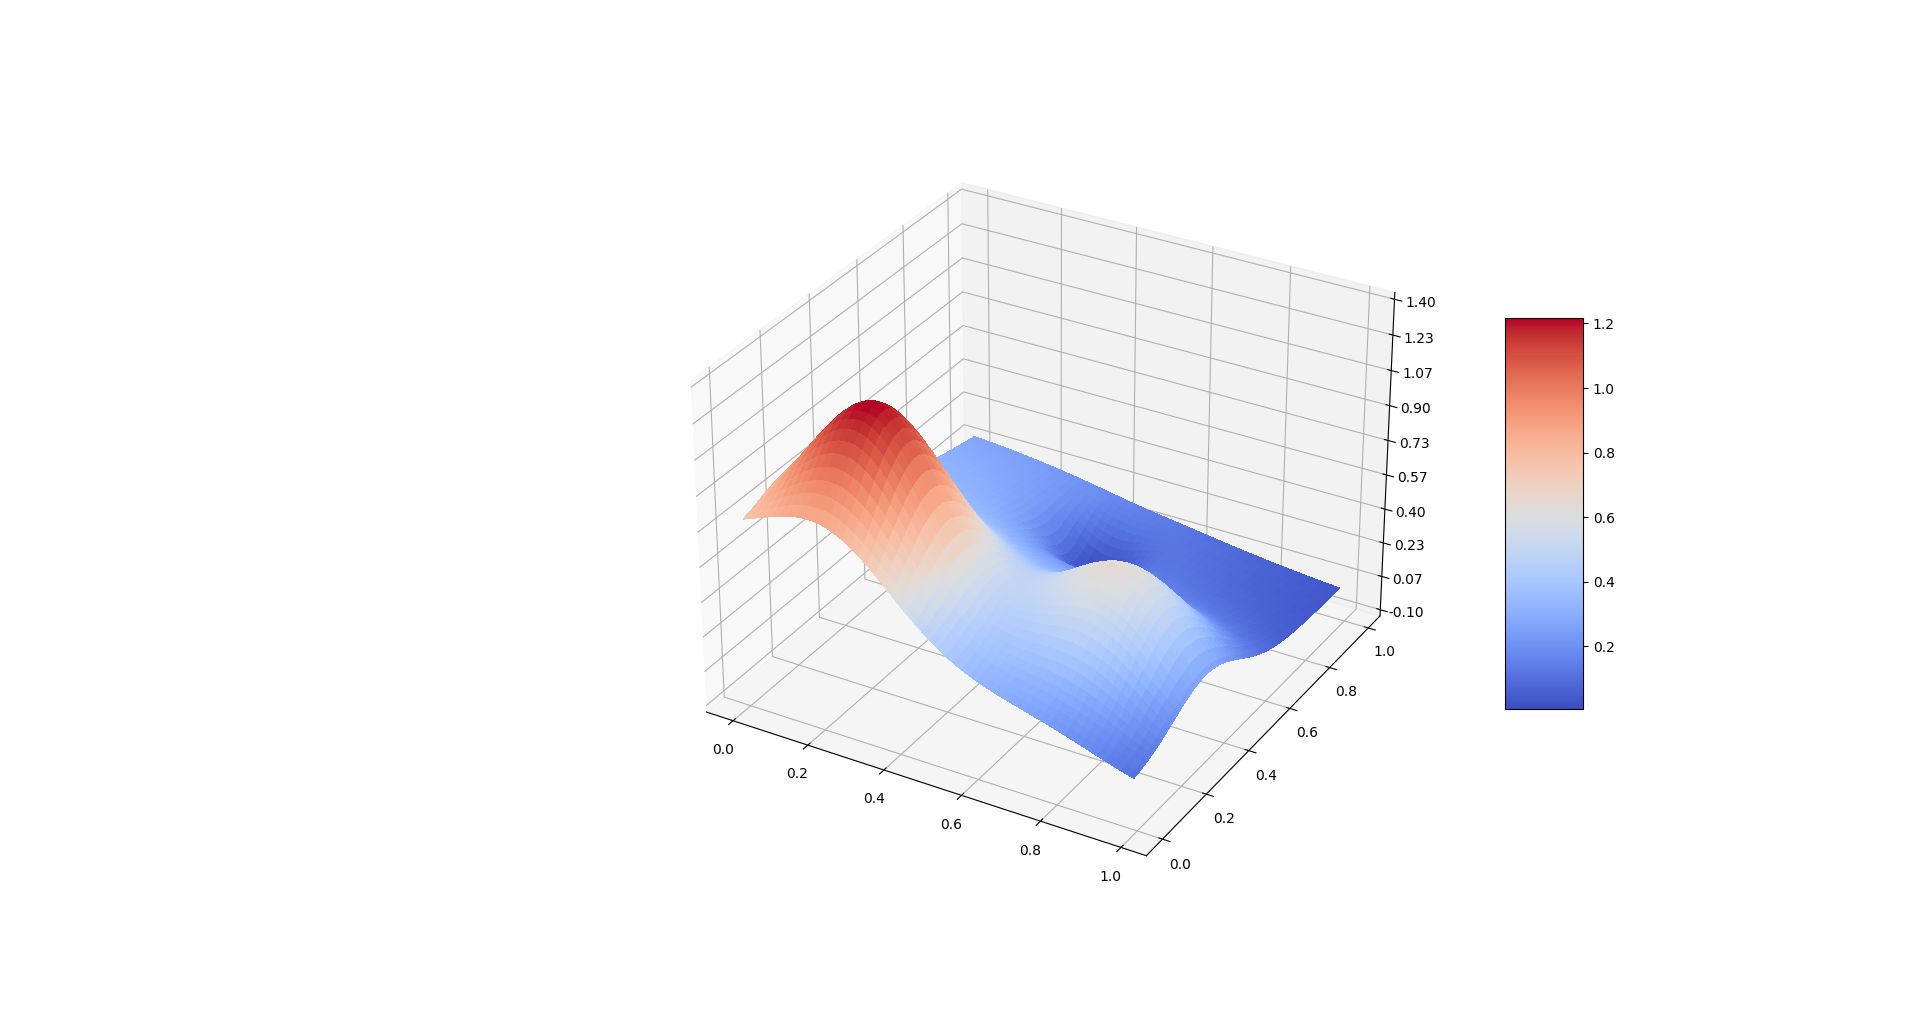
\includegraphics[width = 1\linewidth]{C:/Users/Sander/Documents/GitHub/FYS-STK4155/Project1/Report/Figures/zReal_n100_p5_noise0001_ts025.PNG}
\caption{\label{fig:FrankeReal2} The real Franke function when we have $100$ observations and polynomials of degree $5$ using a noise-level of $0.001$ and a $75/25$ train/test split.}
\end{figure}

\begin{figure}[H]
\centering
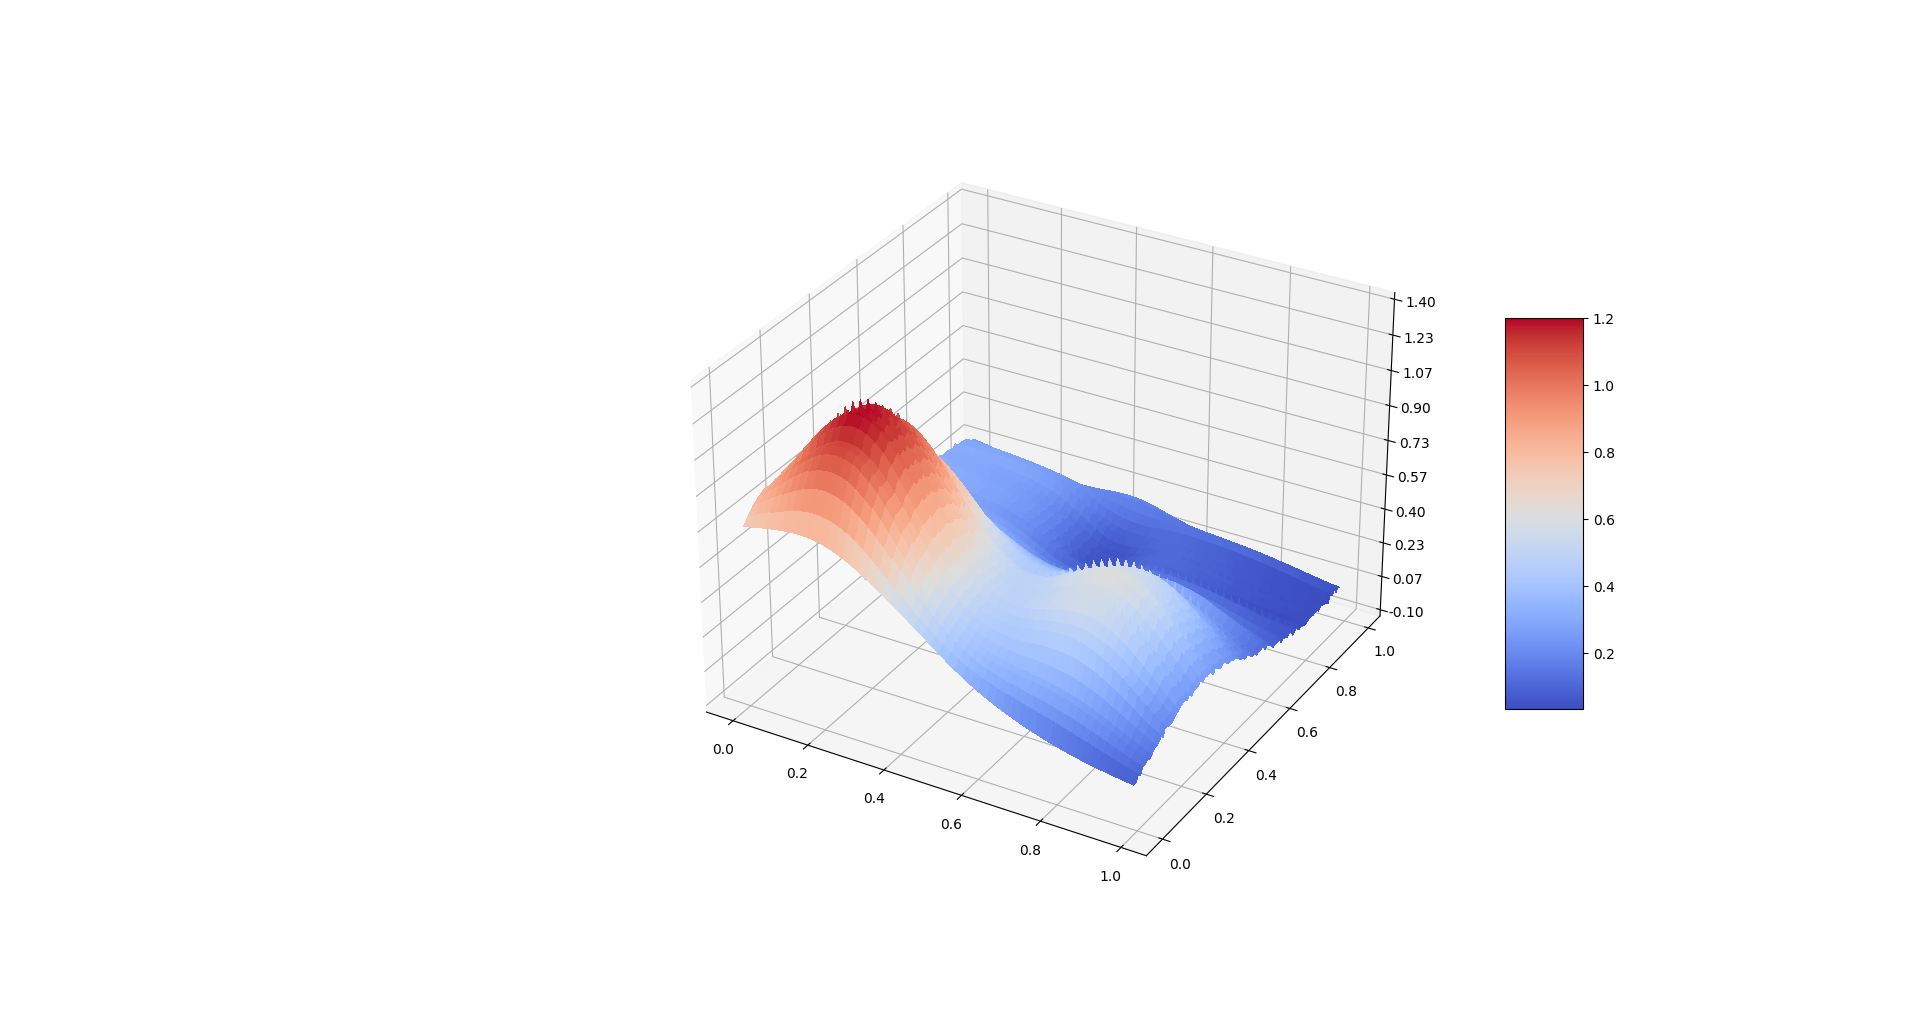
\includegraphics[width = 1\linewidth]{C:/Users/Sander/Documents/GitHub/FYS-STK4155/Project1/Report/Figures/zEst_n100_p5_noise0001_ts025.PNG}
\caption{\label{fig:FrankeEst2} The estimated Franke function when we have $100$ observations and polynomials of degree $5$ using a noise-level of $0.001$ and a $75/25$ train/test split.}
\end{figure}

\begin{figure}[H]
\centering
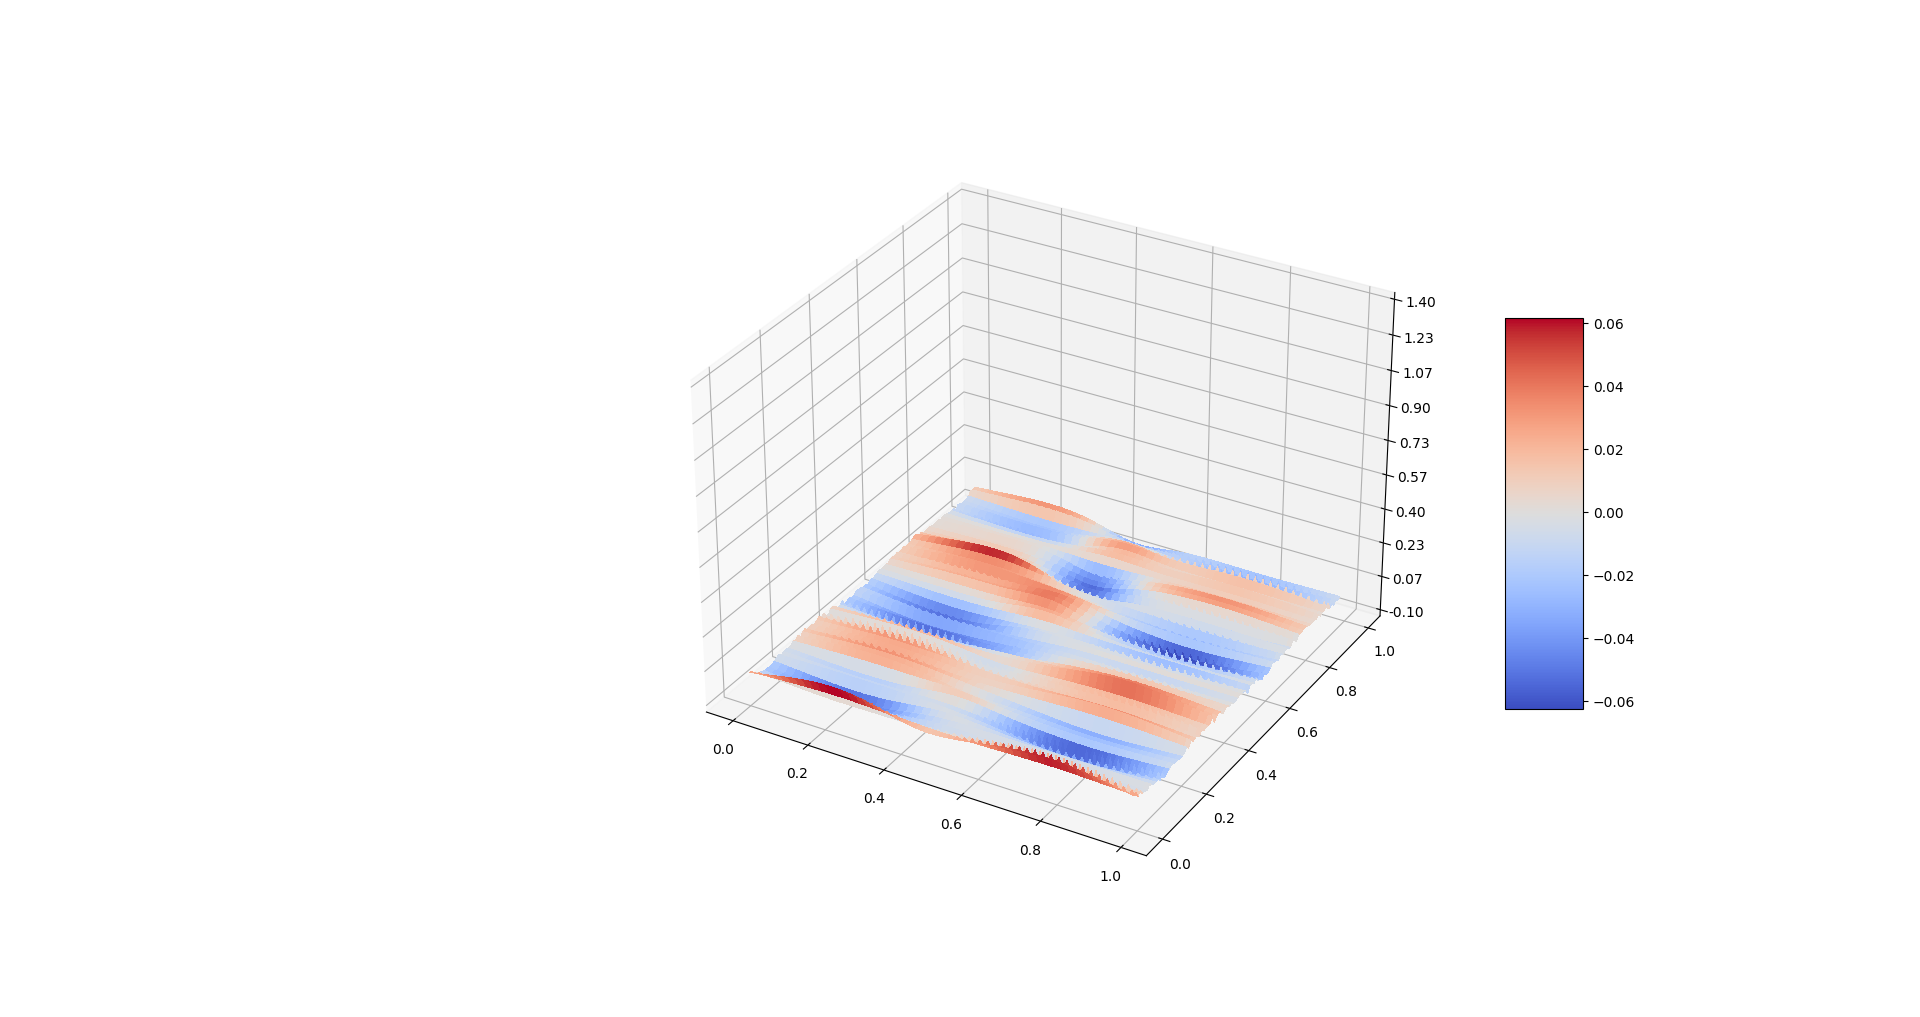
\includegraphics[width = 1\linewidth]{C:/Users/Sander/Documents/GitHub/FYS-STK4155/Project1/Report/Figures/zDiff_n100_p5_noise0001_ts025.PNG}
\caption{\label{fig:FrankeDIFF2} The difference between the real and estimated Franke functions when we have $100$ observations and polynomials of degree $5$ using a noise-level of $0.001$ and a $75/25$ train/test split.}
\end{figure}

\noindent We first observe that the figure is much smoother than the previous ones, as the function is discretized by n. We can again get a better understanding of these plots by finding the MSE and $R^2$ as shown in table \ref{tab:ESTREAL2}

\begin{table}[h]
\caption{\label{tab:ESTREAL2} MSE and $R^2$ between the real and estimated Franke function when we have $100$ observations and polynomials of degree $5$ using a noise-level of $0.001$ and a $75/25$ train/test split.}
\centering
\begin{tabular}{c|c|c}
 & MSE & $R^2$\\
\hline
Training & $0.000565152580116653$ & $0.9935076041084075$\\
\hline
Test & $0.0008407777639833455$ & $0.9865450620944748$\\	  
\end{tabular}
\end{table}

\noindent At first glance, one may panic as the training MSE and $R^2$ is lower than for $n= 10$. However, this value is not interesting as it is the test MSE that dictates how well the model performs. This is because we are only interested in how well our model is in predicting new data, which it has not trained on, and as we can see from table \ref{tab:ESTREAL2}, both the test MSE and test $R^2$ is much higher with $n = 100$ than with $n = 10$. Therefore it is safe to say that increasing the number of observations drastically increases the predictive ability of the model. 
\\
Furthermore, we can compare figure \ref{fig:betaIntALL2} and figure \ref{fig:betaIntALL1} to see that the confidence of our regression coefficients increase as we increase n. This is actually the reason why the model improves.

\begin{figure}[H]
\centering
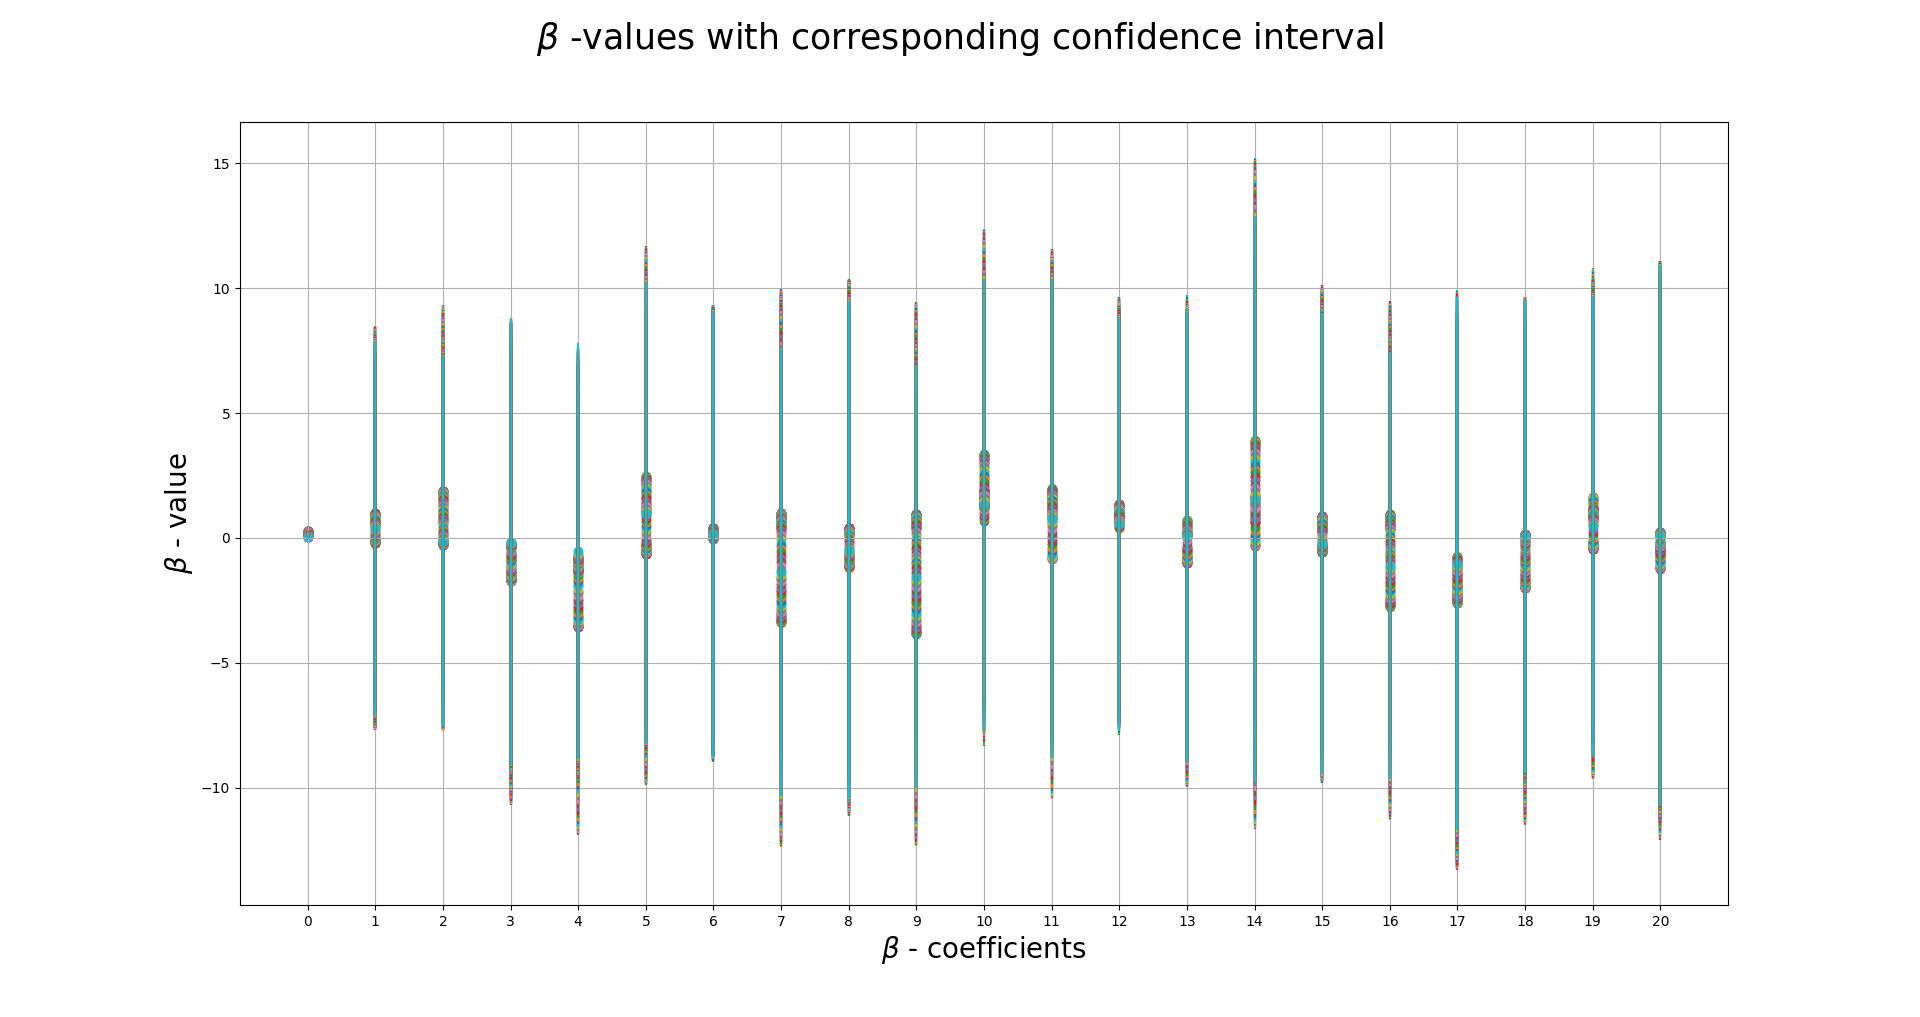
\includegraphics[width = 1\linewidth]{C:/Users/Sander/Documents/GitHub/FYS-STK4155/Project1/Report/Figures/betaInterval_ALL_n100_p5_noise0001_ts025.PNG}
\caption{\label{fig:betaIntALL2} $\hat{\boldsymbol{\beta}}$-coefficients from performing ordinary least squares regression. Dots indicate the actual $\hat{\boldsymbol{\beta}}$-coefficients value while bars around indicate the confidence interval ($\pm \sigma$).}
\end{figure}

\noindent We can also see what happen if we were to increase the noise-level from $0.001$ to $0.1$ using $n = 100$ observations in figures \ref{fig:FrankeEst3}

\begin{figure}[H]
\centering
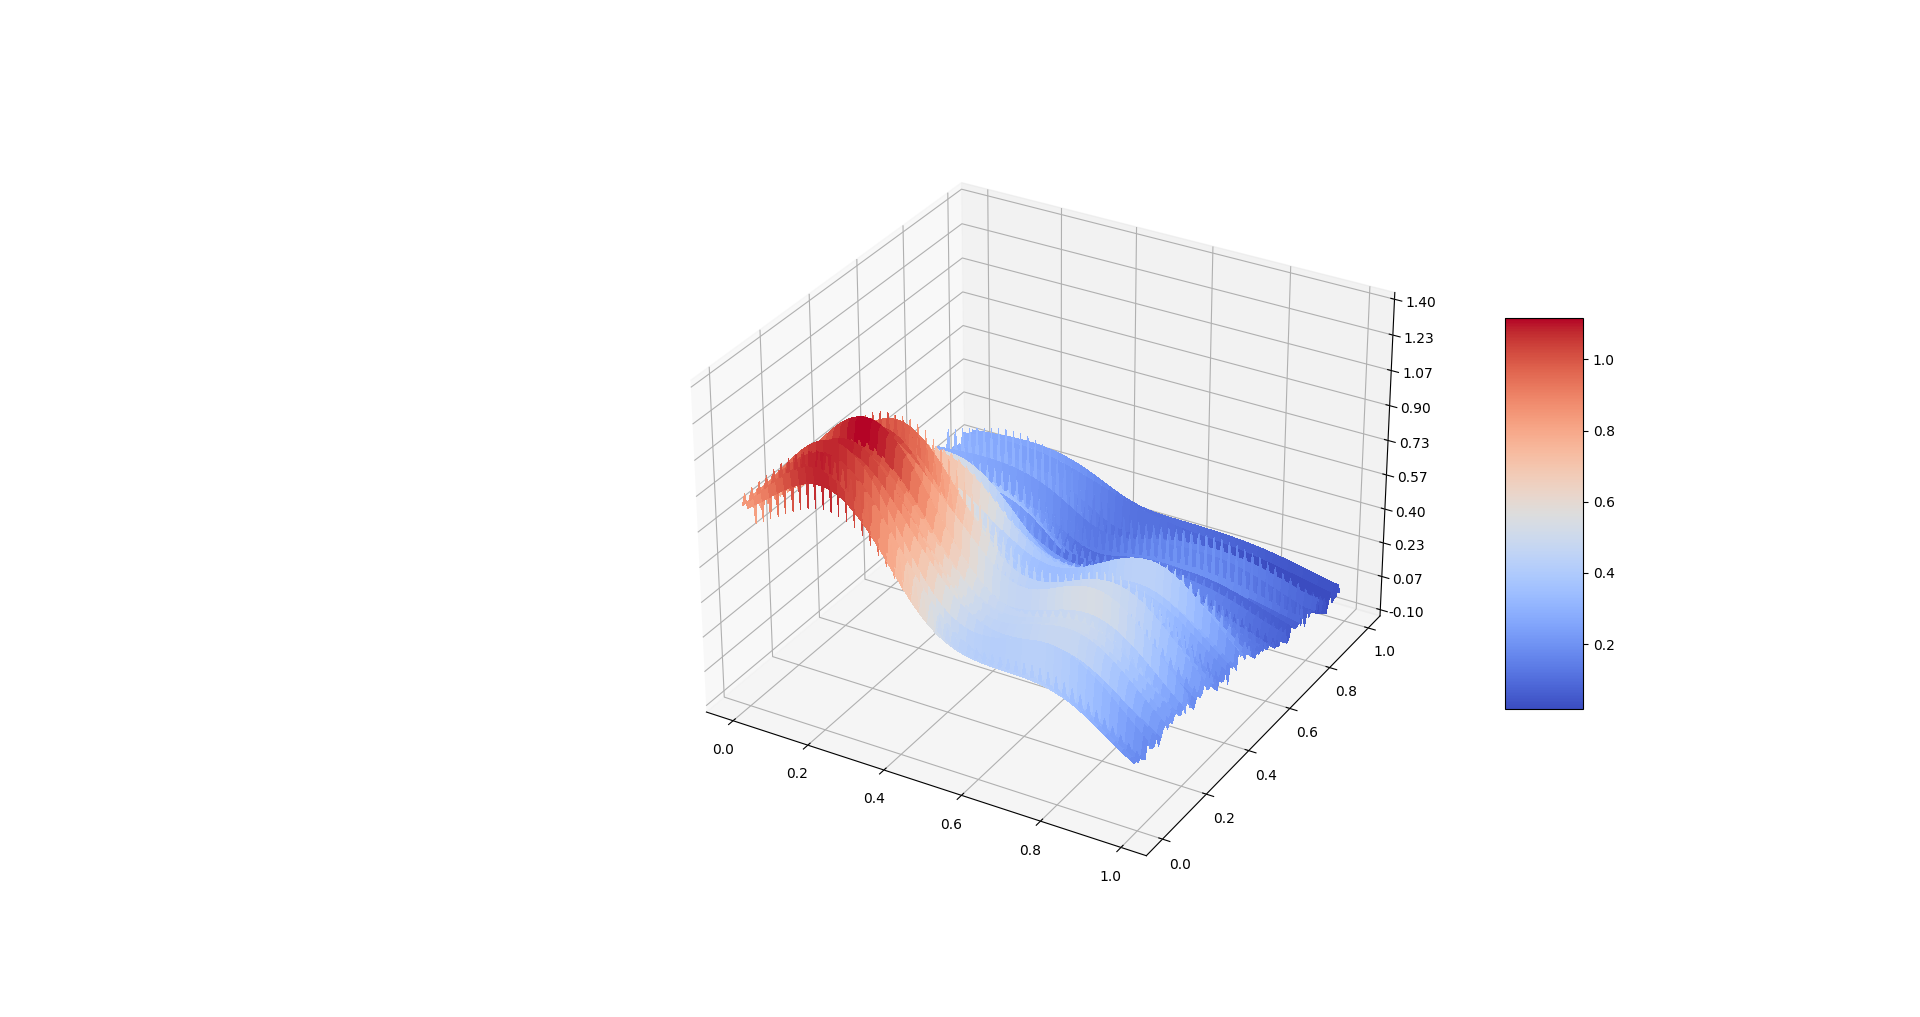
\includegraphics[width = 1\linewidth]{C:/Users/Sander/Documents/GitHub/FYS-STK4155/Project1/Report/Figures/zEst_n100_p5_noise01_ts025.PNG}
\caption{\label{fig:FrankeEst3} The estimated Franke function when we have $100$ observations and polynomials of degree $5$ using a noise-level of $0.1$ and a $75/25$ train/test split.}
\end{figure}

\noindent As expected, the noise makes the model worse at predicting $\hat{y}$. However, the overall traits of the Franke function can still be observed, but the errors shown in table \ref{tab:ESTREAL3} indicates that the performance is worse with more noise

\begin{table}[h]
\caption{\label{tab:ESTREAL3} MSE and $R^2$ between the real and estimated Franke function when we have $100$ observations and polynomials of degree $5$ using a noise-level of $0.1$ and a $75/25$ train/test split.}
\centering
\begin{tabular}{c|c|c}
 & MSE & $R^2$\\
\hline
Training & $0.0075270297407231375$ & $0.9044112376567826$\\
\hline
Test & $0.009241122769969749$ & $0.9012627398304937$\\	  
\end{tabular}
\end{table}

\noindent We could easily remove all the noise from the mode, but we intend to keep a noise level of $0.001$ as it will prepare us for the real data later in the project.

\newpage

\noindent \textbf{b)} When we fit a linear model like in the last exercise, we always want to minimize the mean square error (MSE) of the test set. We can explain the MSE from equation \ref{eq:MSE} in terms of the expected value of its such that the MSE is simply the expected value of the difference between the actual response and the predicted response using regression. This mean we can write the MSE as $E[(y-\hat{y})^2]$ where y is the actual response while $\hat{y}$ is the predicted response (as we already know). By adding and subtracting the term $E[\hat{y}]$ to the inner bracket we can expand the MSE like in equation \ref{eq:mseDerive}

\begin{equation}\label{eq:mseDerive}
\begin{aligned}
MSE = E[(y-\hat{y})^2] = E[(y-\hat{y} + E[\hat{y}] - E[\hat{y}])^2]
\\
E[(\hat{y} - E[\hat{y}])^2 + 2(\hat{y} - E[\hat{y}])(E[\hat{y}]-y) + (E[\hat{y}]-y)^2]
\\
E[(\hat{y} - E[\hat{y}])^2] + E[2(\hat{y} - E[\hat{y}])(E[\hat{y}]-y)] + E[(E[\hat{y}]-y)^2]
\end{aligned}
\end{equation}

\noindent Since the expected value of $\hat{y}$ equals y when n is large, we can write $E[\hat{y}] - y =$ constant and thus

\begin{equation}\label{eq:mseDerive2}
\begin{aligned}
E[(\hat{y} - E[\hat{y}])^2] + 2(E[\hat{y}]-y)E[\hat{y}-E[\hat{y}]] + (E[\hat{y}]-y)^2
\\
E[(\hat{y} - E[\hat{y}])^2] + 2(E[\hat{y}]-y)(E[\hat{y}] - E[\hat{y}])+ (E[\hat{y}]-y)^2
\\
E[(\hat{y} - E[\hat{y}])^2] + (E[\hat{y}]-y)^2
\end{aligned}
\end{equation}

where the constant $E[\hat{y}] - E[\hat{y}]$ equals zero, making the whole term equal zero. 
\\
We recognize the term $E[(\hat{y} - E[\hat{y}])^2]$ as the variance of estimator $\hat{y}$ and the term $(E[\hat{y}]-y)^2$ as the bias of the model, but squared. The bias quantifies how well the model fits the data points and variance is how well the model would translate to other data the model is not trained on. Increasing one tends to decrease the other, but not linearly since the bias is squared. Therefore, one can decrease the bias to a certain extent, but at some point, the loss of bias is not worth the gain in variance. This is called the bias variance trade-off. 
\\
Before investigating the bias-variance trade-off any further, we need to solve a problem related to the lack of data that is often the case with real data. When we generate data synthetically, the lack of data is never a problem, but in the real world, data is always limited and we now want to simulate that experience. Imagine now that we only have 100 observations and that these 100 observations are enough to represent the underlying distribution of the data, but not enough for our machine learning algorithm to function properly. We can then utilize the bootstrap resampling method to create data out of thin air. The bootstrap resampling method aims to take the original data of size n and create B new data sets each of size n. This is done by randomly assigning observations from the original data set to the B new data sets (with replacement). Then, a statistic is calculated for each of the B new data sets and the mean of all these statistics should represent the statistic of the original data set. The new statistic is often called the bootstrap statistic and will in this report be the MSE. Figure \ref{fig:Bootsketch} shows a rough sketch of the process

\begin{figure}[H]
\centering
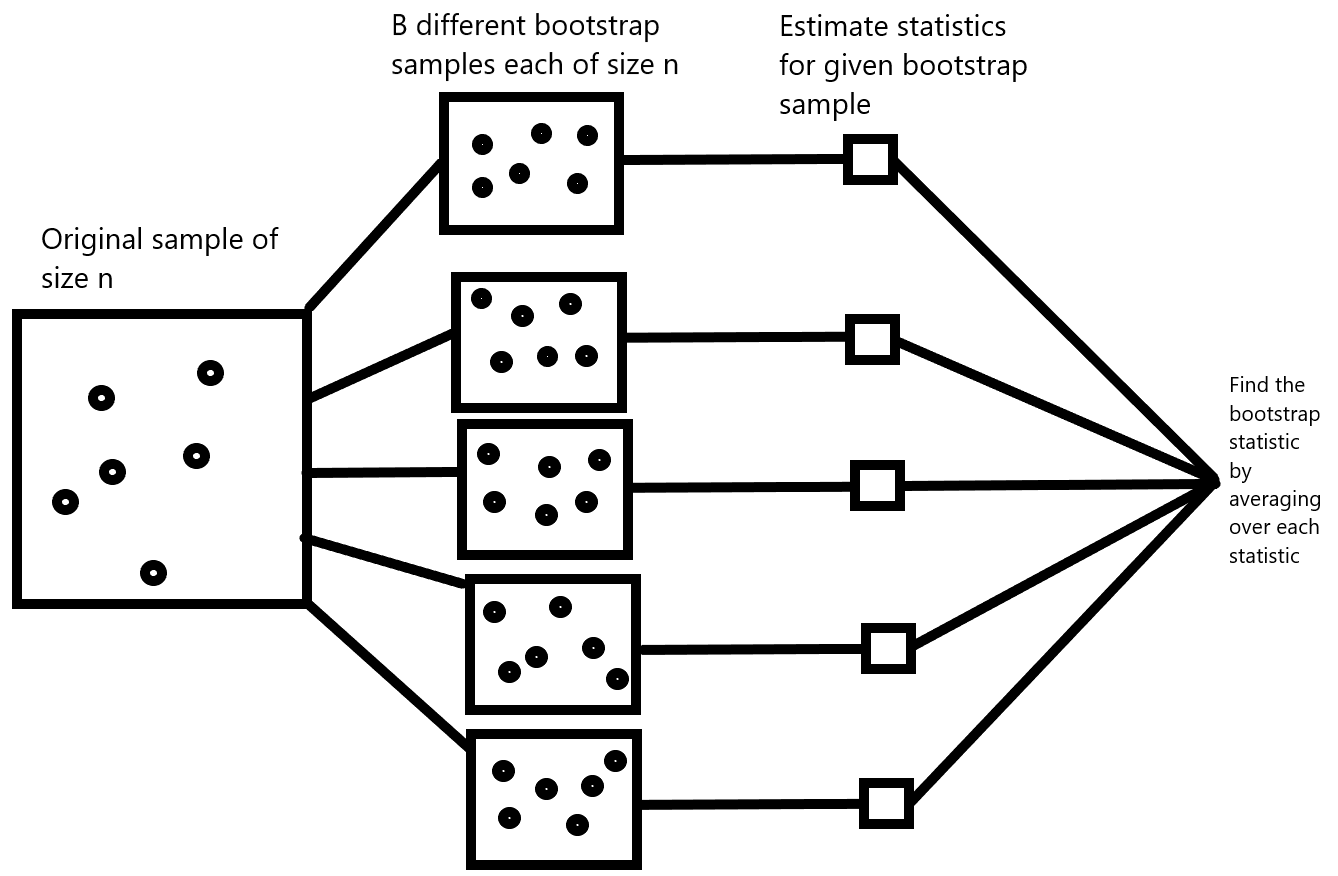
\includegraphics[width = 1\linewidth]{C:/Users/Sander/Documents/GitHub/FYS-STK4155/Project1/Report/Figures/bootstrapSketch.PNG}
\caption{\label{fig:Bootsketch} Illustration of the bootstrap process. The statistic in question here is the MSE.}
\end{figure}

\noindent The hope of the bootstrap method is that the bootstrap statistic represents the statistic of the underlying distribution of the original data set, regardless of the original datasets distribution. Be aware, the bootstrap method does not create new information, but simply exaggerate the already existing information, letting us perform operations like linear regression more easily.
\\
Now that we have a method of creating more data, we can study the bias-variance trade-off more thoroughly. More spesifically, we want to study how the bias, variance and MSE changes as a function of polynomial degree. Now imagine we just have 100 observations. We can then utilize the bootstrap resampling method to create $B \times n$ more data. Let us generate $B = 100$ data sets each of size n and see how the our parameters of interest change with polynomial degree as seen in figures \ref{fig:MSEBOOT1} and \ref{fig:BVBOOT1}

\begin{figure}[H]
\centering
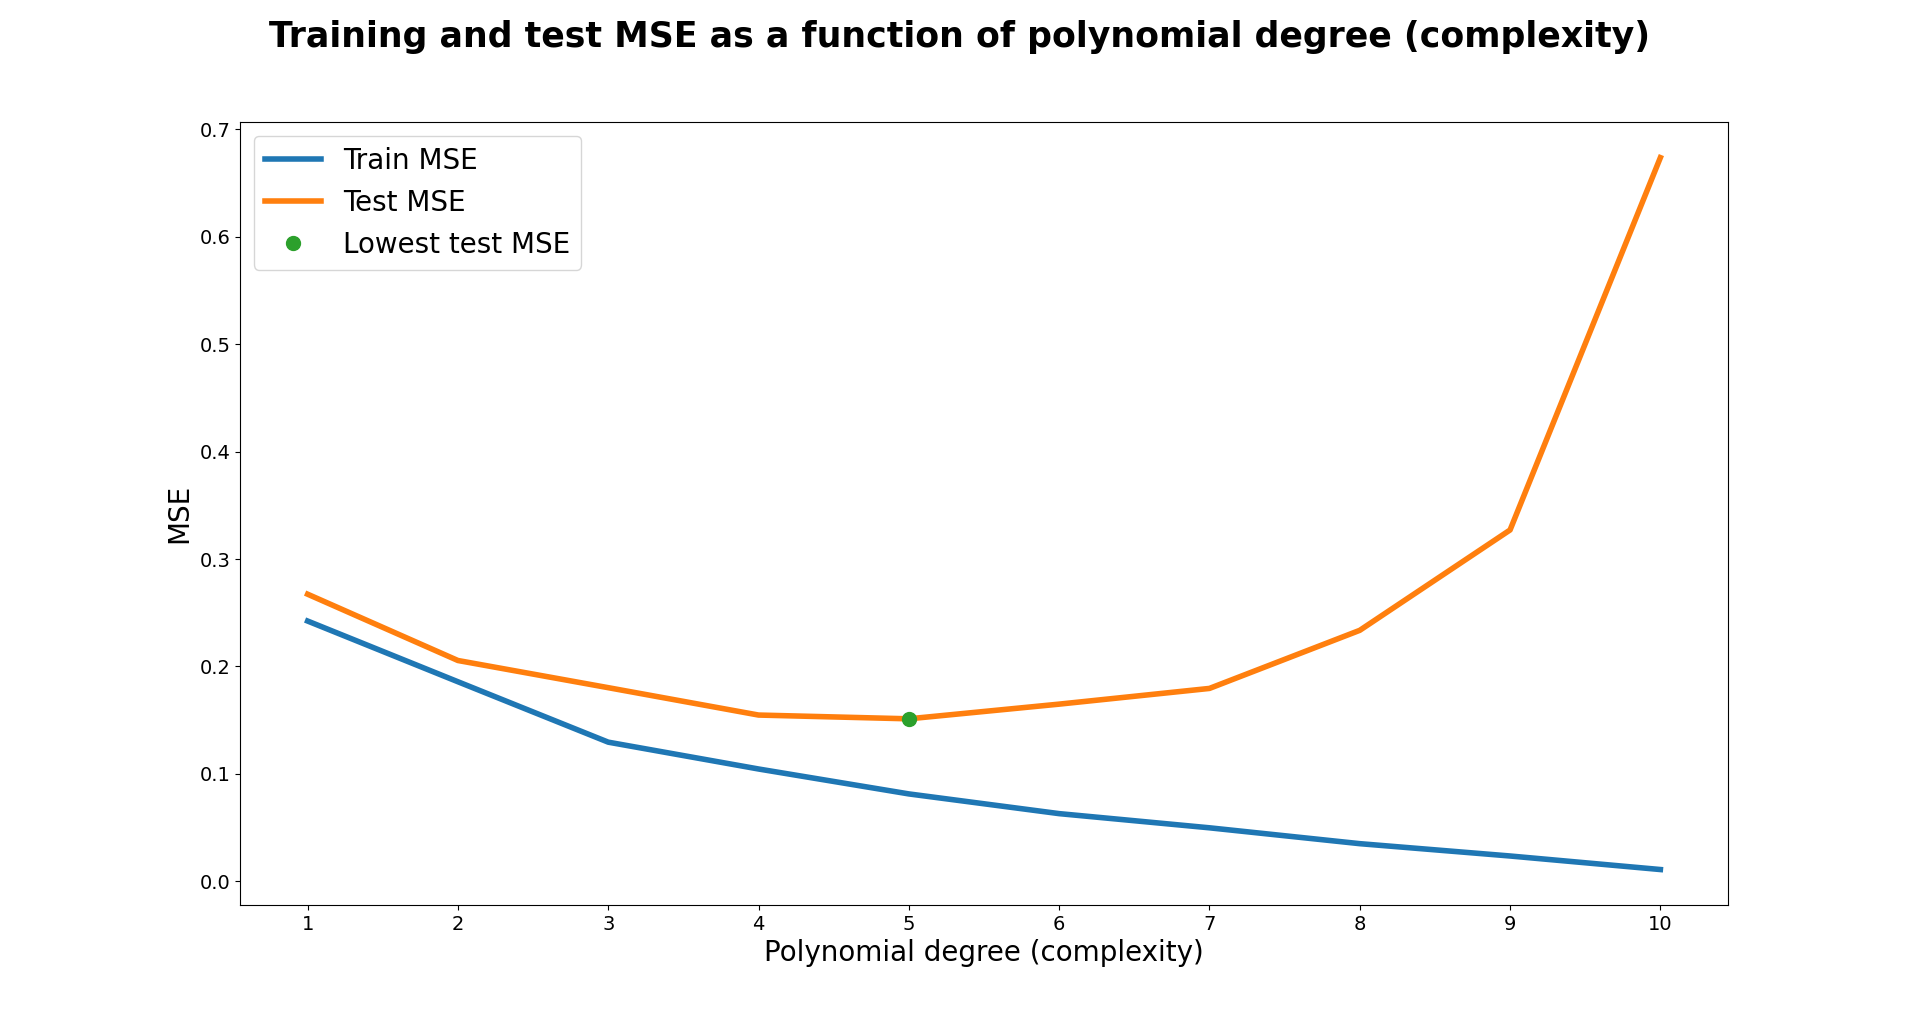
\includegraphics[width = 1\linewidth]{C:/Users/Sander/Documents/GitHub/FYS-STK4155/Project1/Report/Figures/MSEBOOT_n1000_p10_noise0001_ts025_B100_shuffles.PNG}
\caption{\label{fig:MSEBOOT1} MSE as a function of polynomial degree using the bootstrap resampling method. Here we have 100 observations while we generate 100 bootstrap samples with a noise level of $0.001$ and a $75/25$ train test split.}
\end{figure}

\begin{figure}[H]
\centering
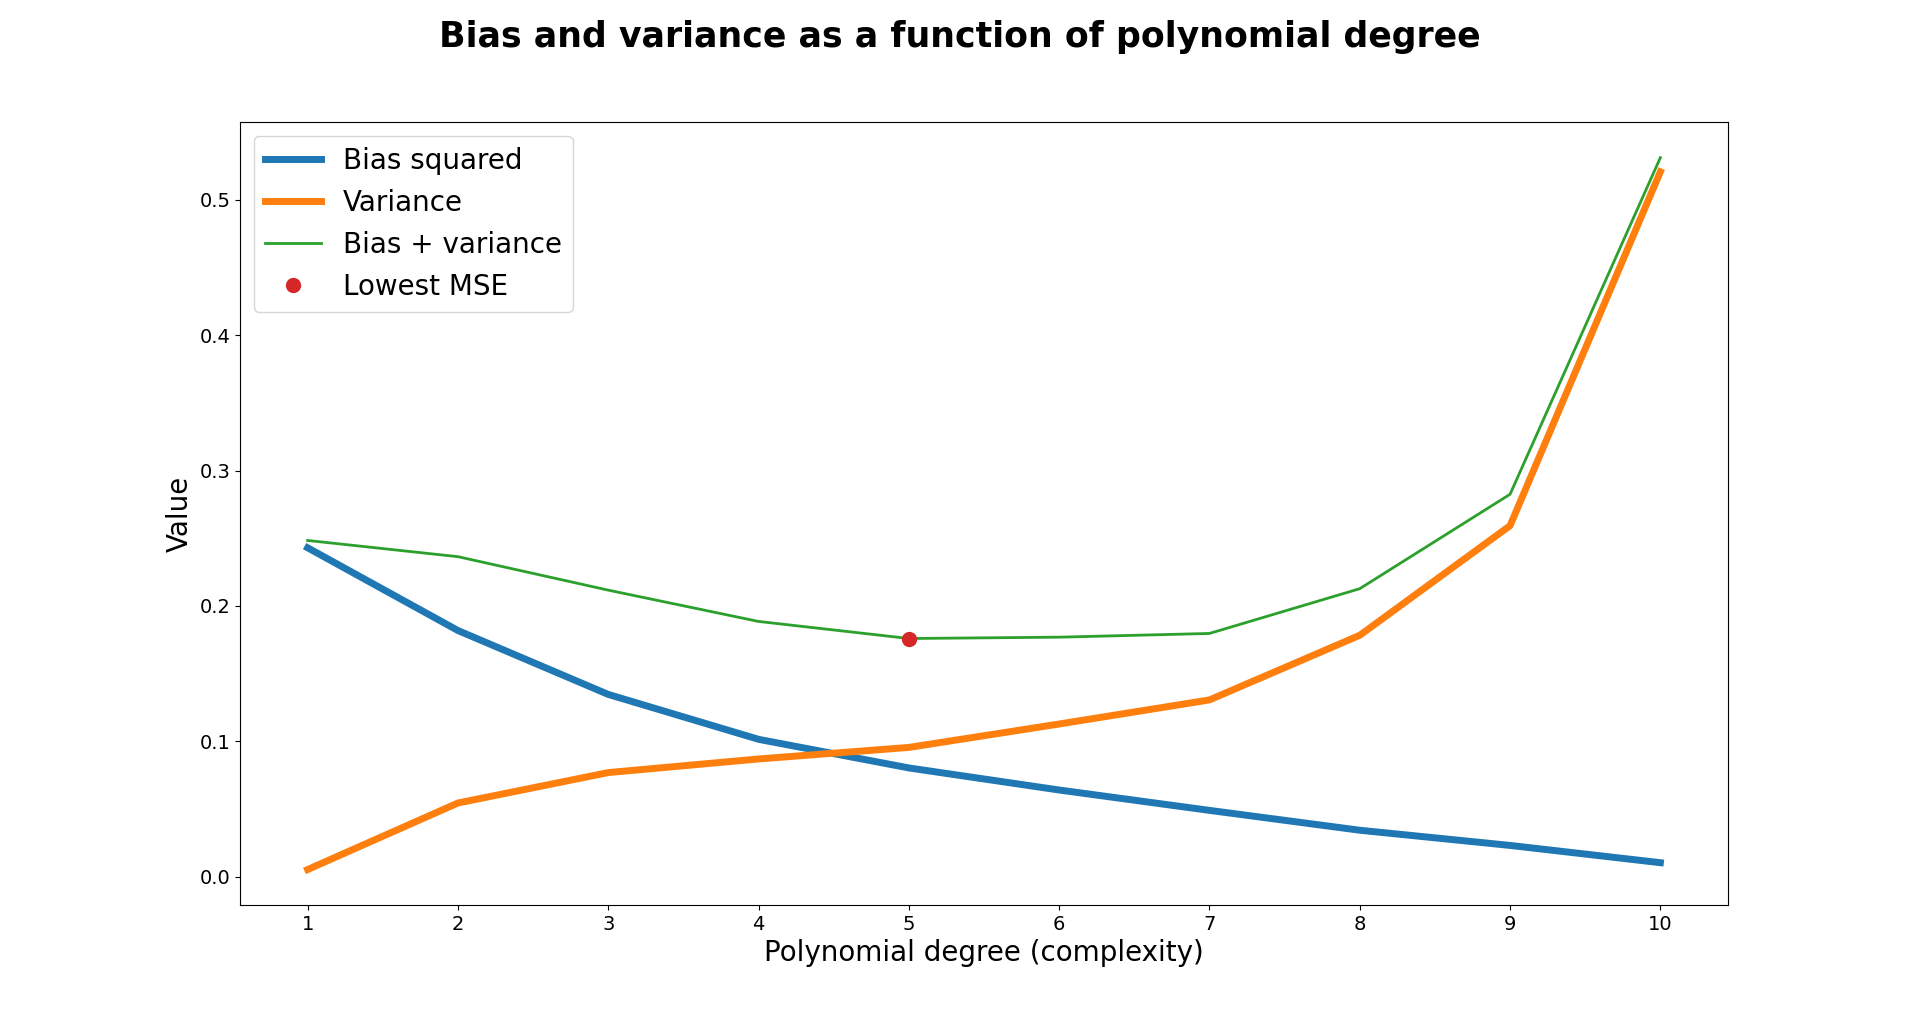
\includegraphics[width = 1\linewidth]{C:/Users/Sander/Documents/GitHub/FYS-STK4155/Project1/Report/Figures/BVplotBOOT_n1000_p10_noise0001_ts025_B100_shuffles.PNG}
\caption{\label{fig:BVBOOT1} Bias and variance decomposition of figure \ref{fig:MSEBOOT1}. The bias and variance change as a function of polynomial degree using the bootstrap resampling method. Here we have 100 observations while we generate 100 bootstrap samples with a noise level of $0.001$ and a $75/25$ train test split.}
\end{figure}

\noindent We can observe that the bias starts high, but tends towards zero when we increase the complexity of our model. This is because a low order polynomial would be unable to fit the complex structure of the Franke function, thus making the difference between our predicted Franke function and the actual Franke function large. With an large increase in polynomial degree, we can fit the model arbitrarily close to the actual Franke function. 
\\
The variance behaves almost the opposite of the bias as it starts very low, but increases exponentially as we increase the complexity. This is because a low order polynomial would manage to somewhat predict the test data, even if the prediction is horrible. When we increase the complexity, the model is unable to accurately predict the test data because the model is over fitting the model to the data of the training set. 
\\
We can also see that the minimum MSE in figure \ref{fig:MSEBOOT1} corresponds to the same polynomial as that of figure \ref{fig:BVBOOT1}, strengthening our trust in the models predictive capabilities, but what would happen if we were to decrease the number of bootstrap samples? Let us now generate a new model where all the parameters are the same as of the previous one, but where we only generate 10 bootstrap samples. Then we get something akin to figure \ref{fig:MSEBOOT2}

\begin{figure}[H]
\centering
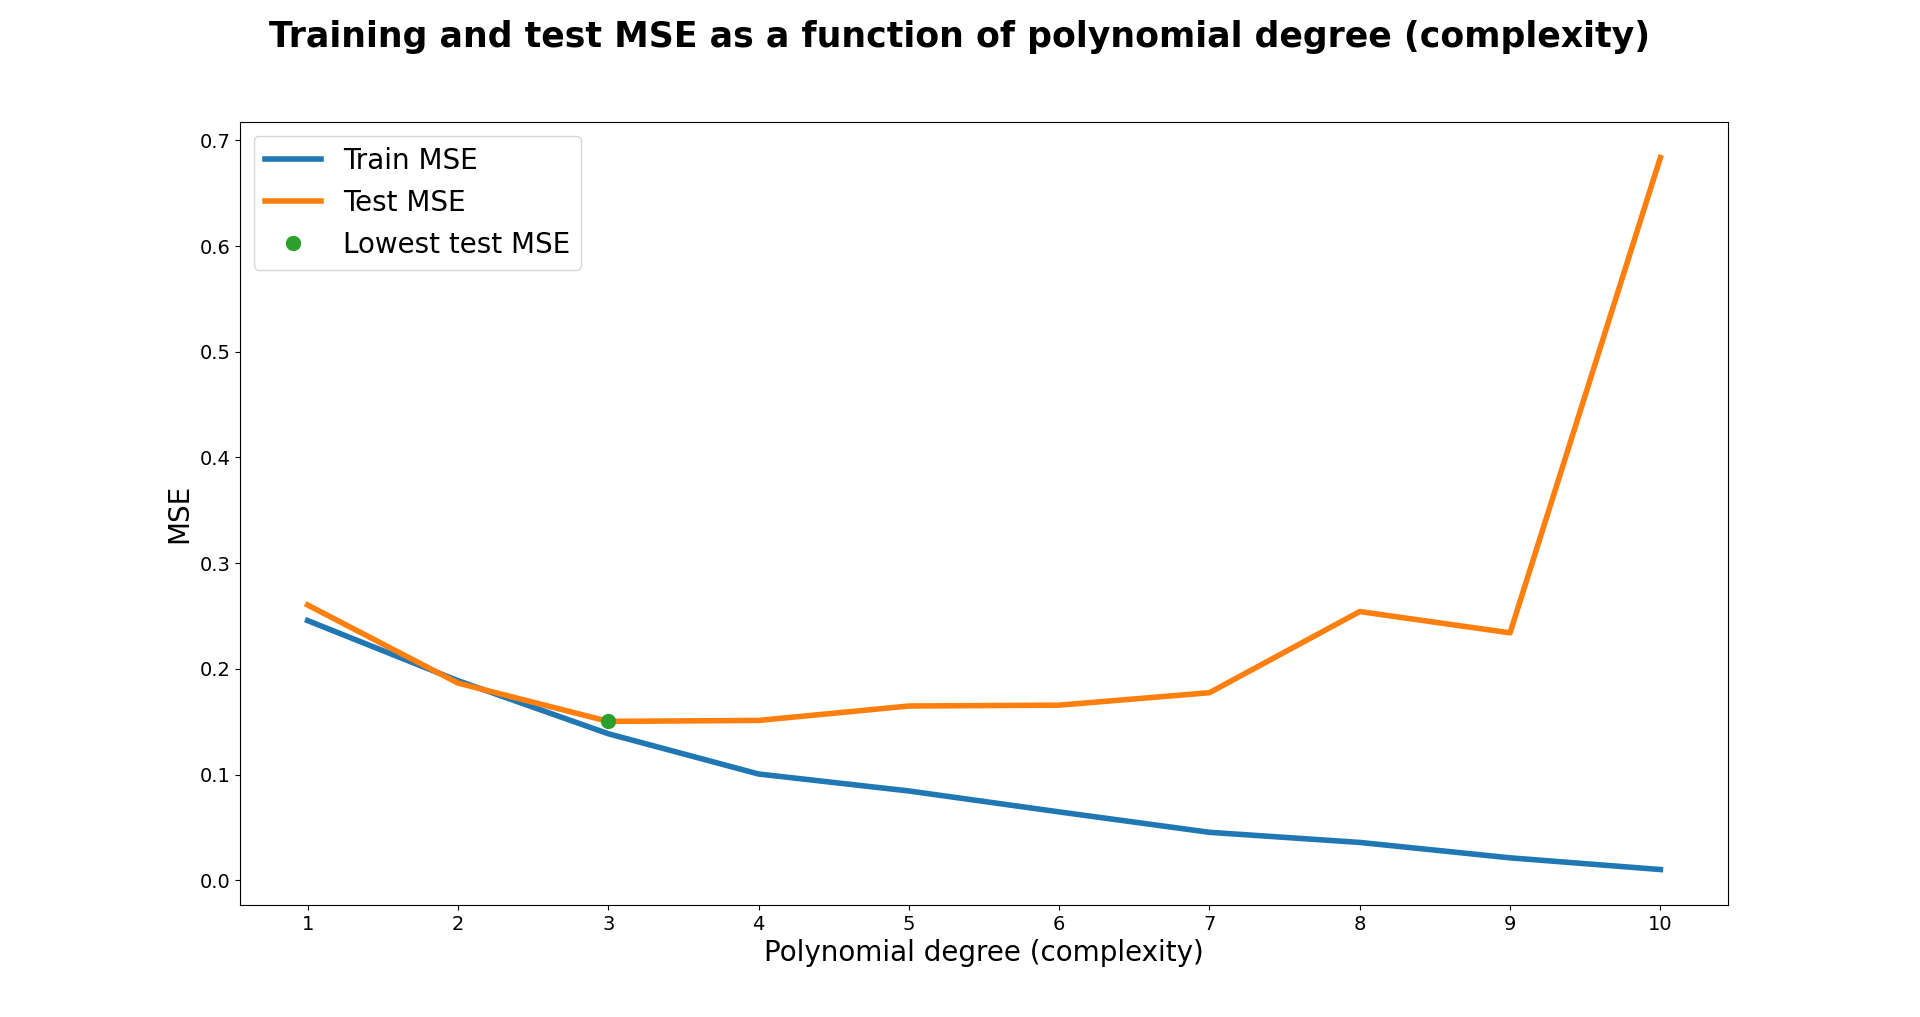
\includegraphics[width = 1\linewidth]{C:/Users/Sander/Documents/GitHub/FYS-STK4155/Project1/Report/Figures/MSEBOOT_n1000_p10_noise0001_ts025_B10_shuffles.PNG}
\caption{\label{fig:MSEBOOT2} MSE as a function of polynomial degree using the bootstrap resampling method. Here we have 100 observations while we generate 10 bootstrap samples with a noise level of $0.001$ and a $75/25$ train test split.}
\end{figure}

\noindent We can observe from figure \ref{fig:MSEBOOT2} that the point of lowest MSE is now at $p = 3$ which is lower than the one observed in figure \ref{fig:MSEBOOT1}. This is because more data means that the model can be trained more without overfitting the model. Thus, when we decrease the number of observations (or bootstrap samples in this case), we lower the threshold for when the model becomes overfit. This again means that a lower degree of polynomial is the ideal complexity for the model. 
\\
What is also observed from the code when using a low amount of bootstrap samples is that the model becomes increasingly unstable. This is because the bootstrap MSE relies on the mean of the B generated statistics. If we only generate a few bootstrap samples, the mean is more prone to randomness, which in turn means the algorithm is unstable. For this reason and the one described above (more data is good), we want to stick with 100 bootstrap samples from here on out.

\newpage

\noindent \textbf{c)} We will now introduce another resampling method called cross-validation (CV) and repeat the analysis of the previous exercise. The cross-validation resampling method, like the bootstrap, also aims to create more data out of thin air. However, the process is quite different than that of the bootstrap. The main idea behind the CV is to divide the original data set into k different data sets, or folds as they are called, and then let the kth fold act as the test set while the other k-1 folds acts as the training sets. A model is then fit for each permutation and a statistic is calculated. Then, another fold will act as the test set while the others will act as the training set. This process repeats until every fold has been used as a test set and a statistic for each permutation is calculated. The average of the k different statistic is then calculated and is said to represent the actual statistic of the original data set. 
\\
It is typical to have 10, 5 or n different folds and the CV process is then referred to as 10-fold, 5-fold and leave one out (LOOCV) cross-validation methods. The LOOCV is a special case of the CV method where each observations acts as the test set once and this process is sketched in figure \ref{fig:CVsketch}

\begin{figure}[H]
\centering
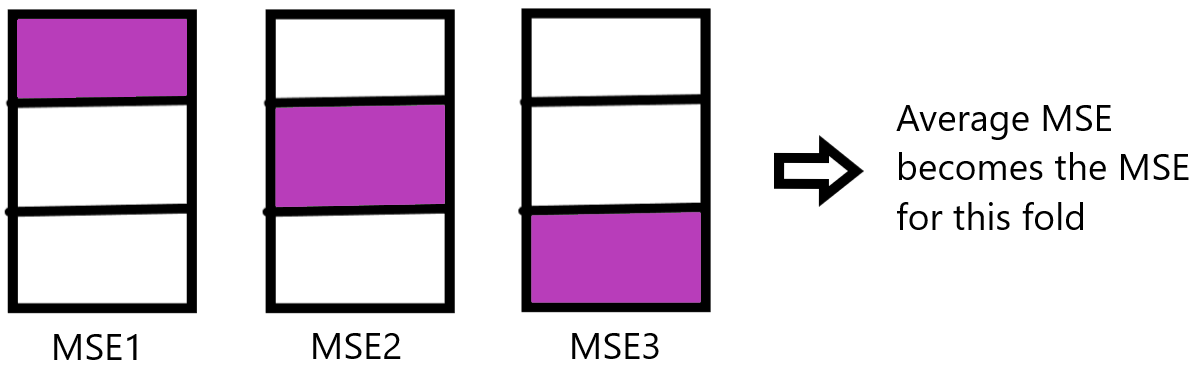
\includegraphics[width = 1\linewidth]{C:/Users/Sander/Documents/GitHub/FYS-STK4155/Project1/Report/Figures/CVSketch.PNG}
\caption{\label{fig:CVsketch} A rough sketch of the LOOCV process. The n observations acts as the test set once (purple squares) while the other $n-1$ observations acts as the training set (white squares). The model is then fit on each distinct permutation and a statistic is calculated (MSE in this project). Finally, an average of the k different statistics is calculated and will represent the statistic of the original data set.}
\end{figure}

\noindent We now want to repeat the process from the previous exercise where we see look at MSE as a function of polynomial degree for the 5-fold, 10-fold and leave one out cross-validations. Let us start with the 10-fold CV which is plotted in figure \ref{fig:MSECV1}

\begin{figure}[H]
\centering
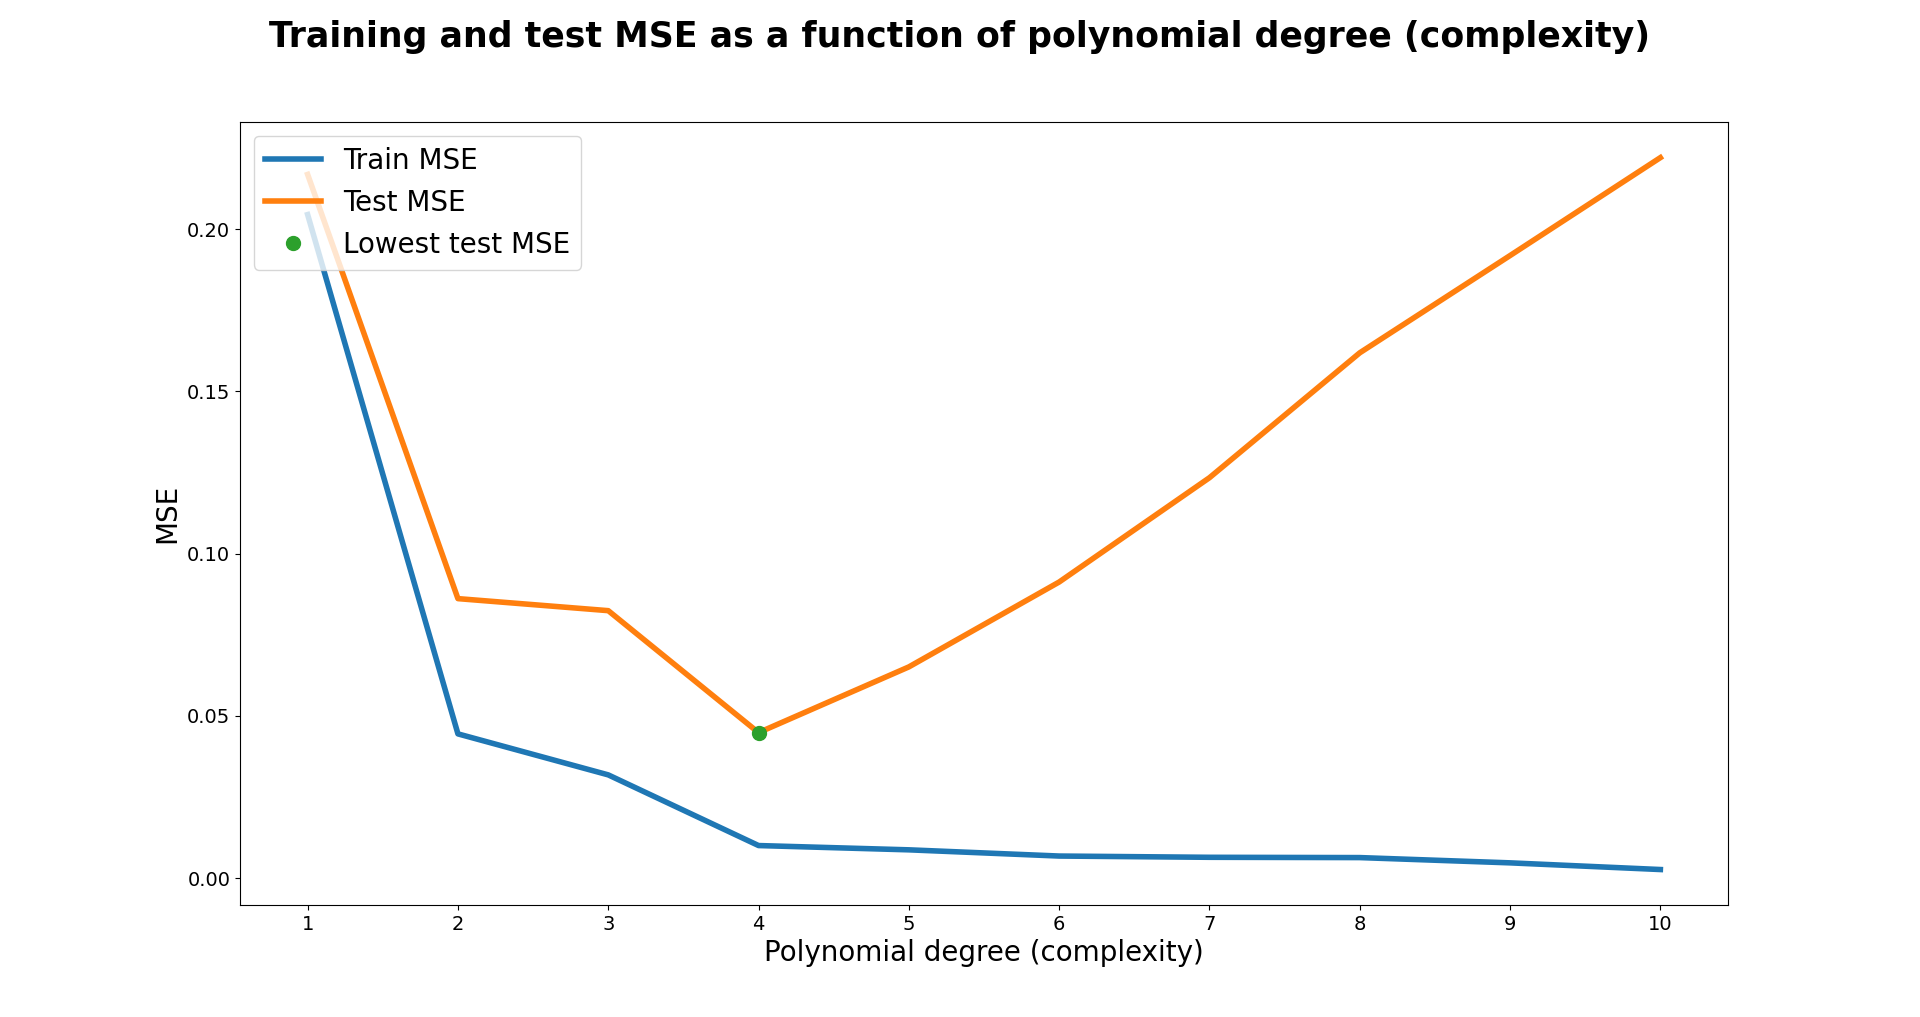
\includegraphics[width = 1\linewidth]{C:/Users/Sander/Documents/GitHub/FYS-STK4155/Project1/Report/Figures/MSECV_n100_p10_noise0001_CV10_shuffles.PNG}
\caption{\label{fig:MSECV1} MSE as a function of polynomial degree up to 10 using the cross-validation resampling method. Here we have 100 observations while we split the data into 10 different folds with a noise level of $0.001$.}
\end{figure}

\noindent We can observe from figure \ref{fig:MSECV1} that the MSE is at its lowest for $p = 4$, similar to the MSE for the bootstrap resampling method in figure \ref{fig:MSEBOOT1}. We can decompose the MSE into its bias and variance components as done in figure \ref{fig:BVCV1}

\begin{figure}[H]
\centering
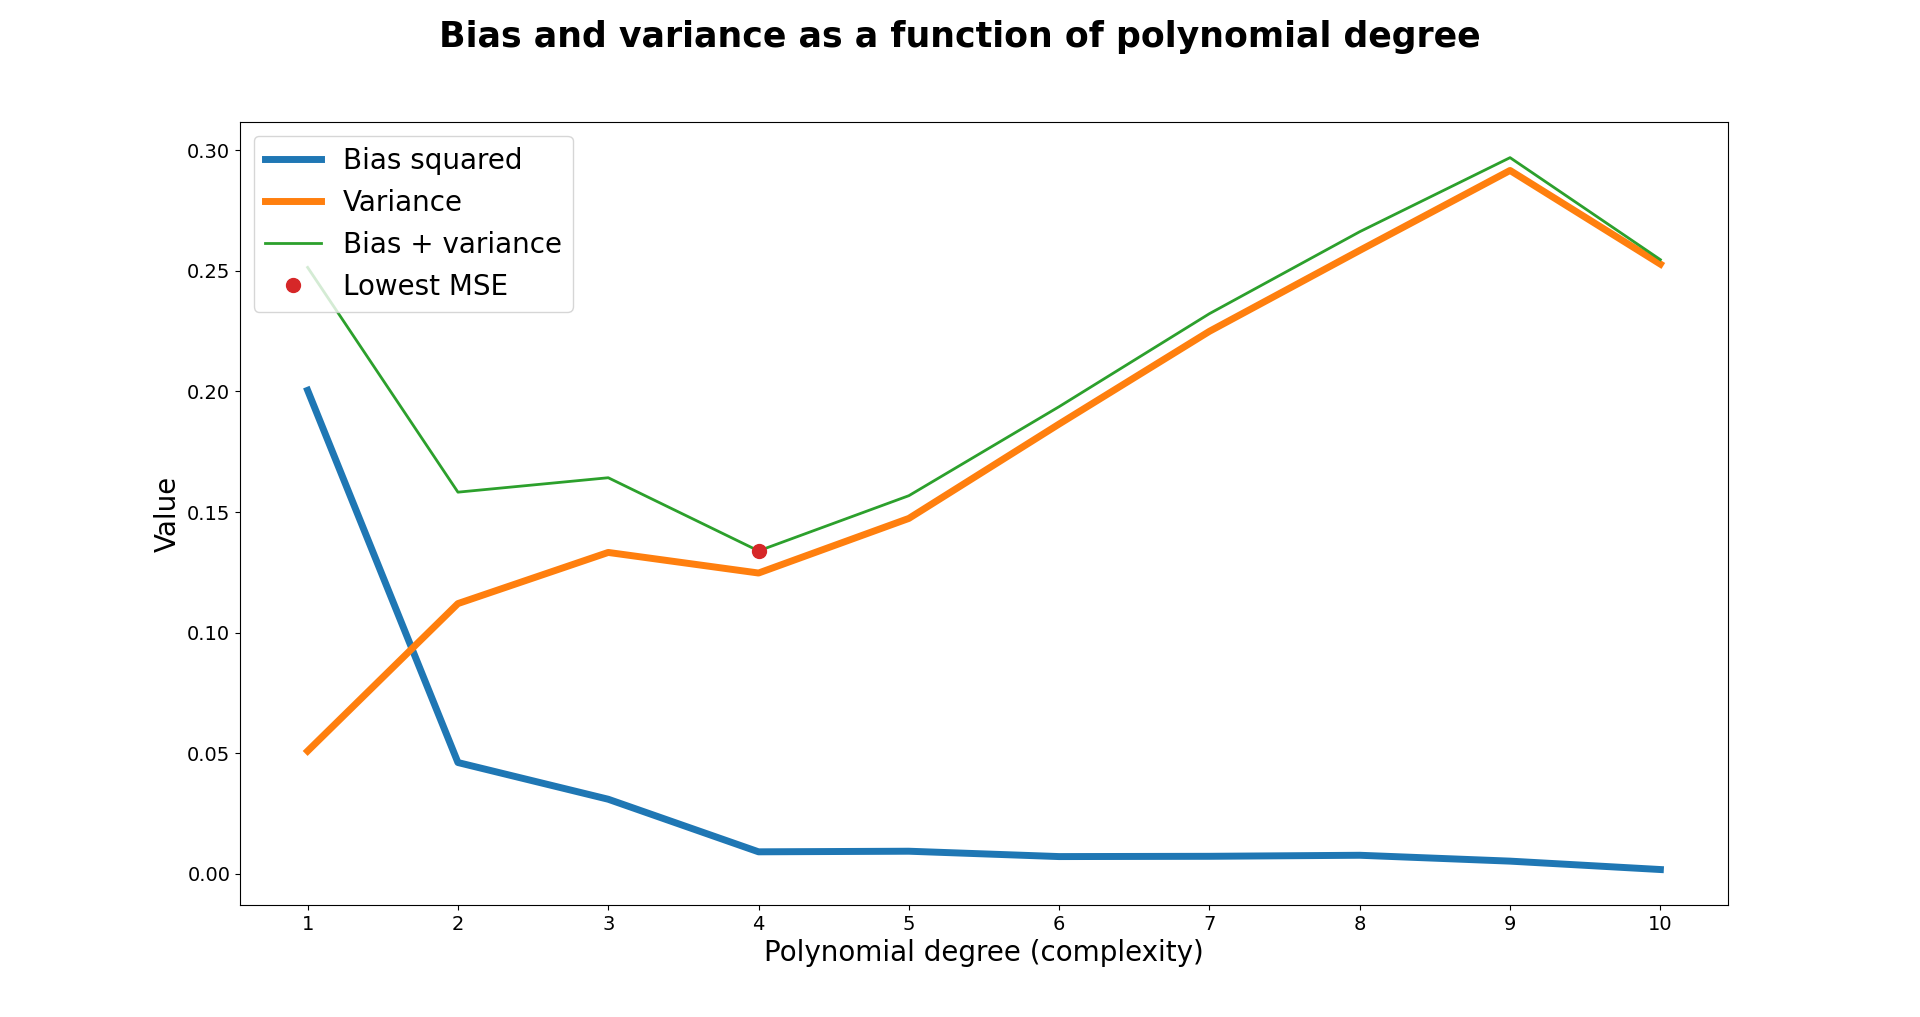
\includegraphics[width = 1\linewidth]{C:/Users/Sander/Documents/GitHub/FYS-STK4155/Project1/Report/Figures/BVplotCV_n100_p10_noise0001_CV10.PNG}
\caption{\label{fig:BVCV1} Bias and variance decomposition of figure \ref{fig:MSECV1}. The bias and variance change as a function of polynomial degree using the CV resampling method. Here we have 100 observations while we use 10-fold CV with a noise level of $0.001$.}
\end{figure}

\noindent It can be confirmed from figure \ref{fig:BVCV1} that the lowest MSE is found at $p = 4$ polynomial degrees. The bias and variance behaves similar to that of bootstrap as seen in figure \ref{fig:BVBOOT1}. 
\\
We now want to see what happens when we set the number of folds k equal to 5 and the result is shown in figures \ref{fig:MSECV2} and \ref{fig:BVCV2}

\begin{figure}[H]
\centering
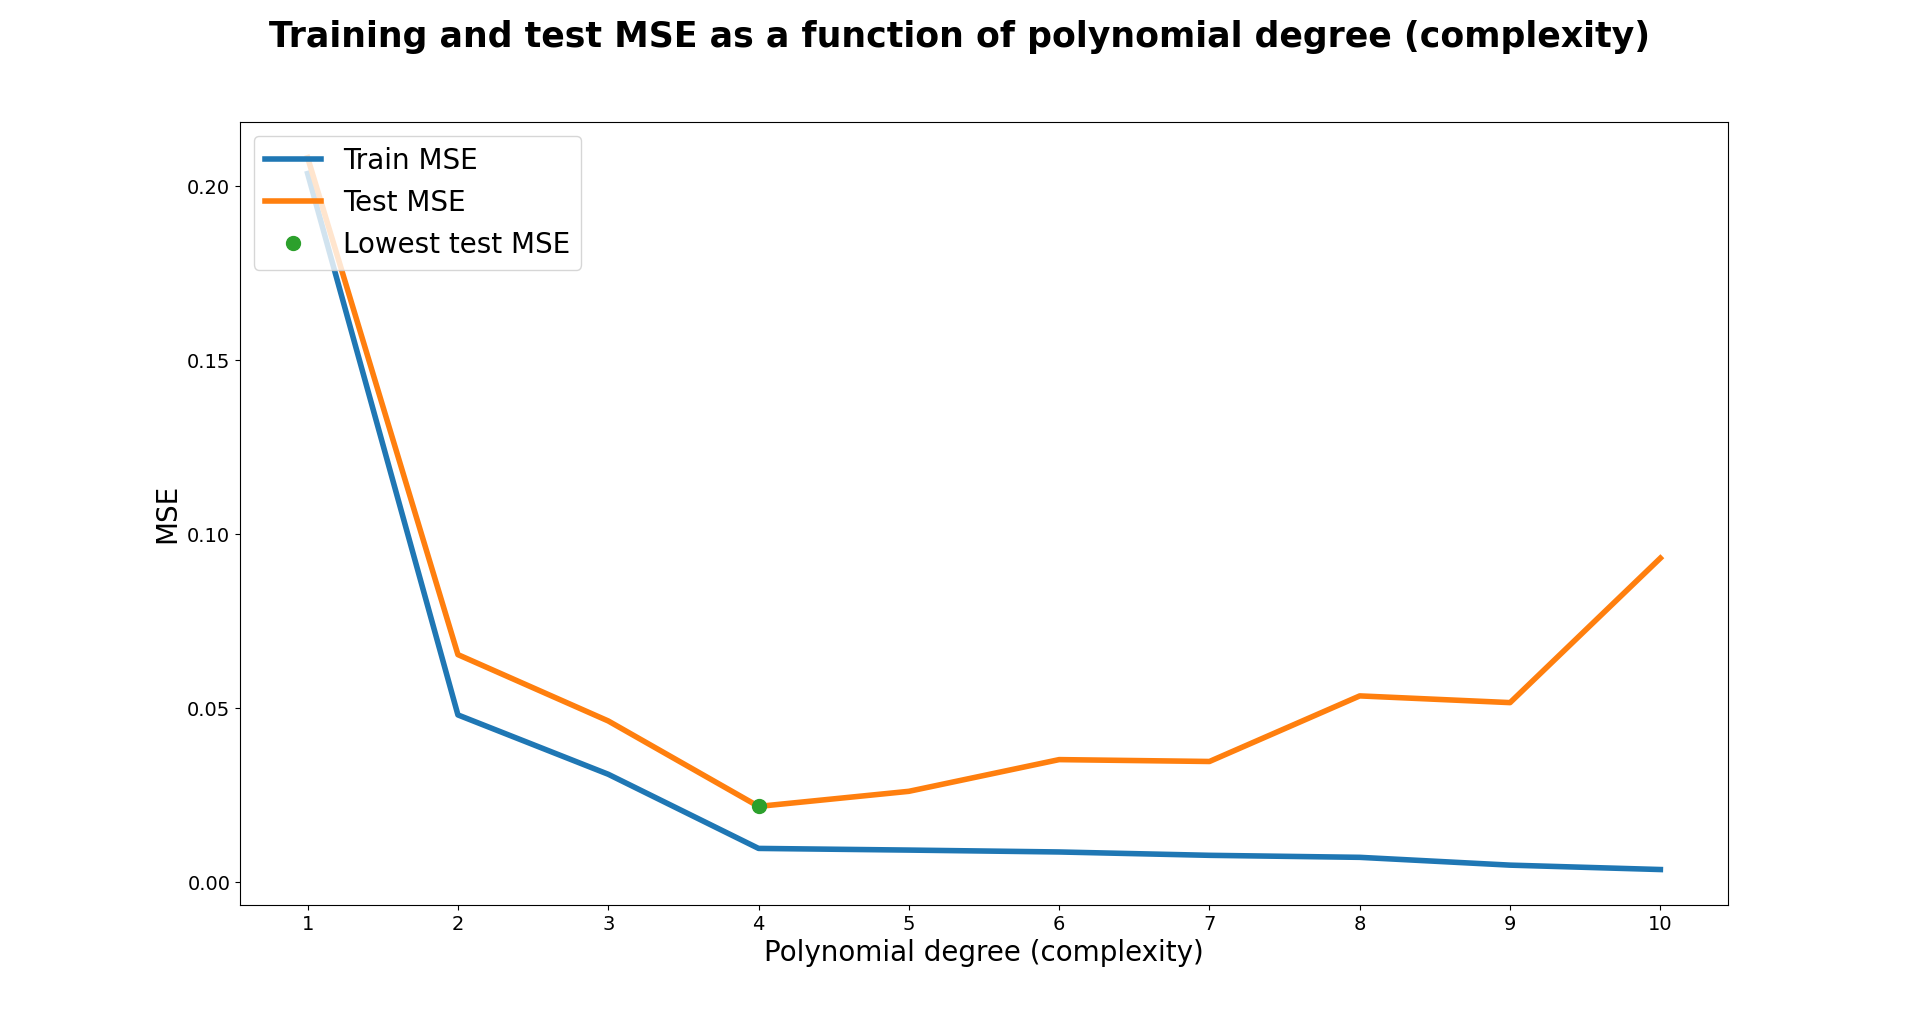
\includegraphics[width = 1\linewidth]{C:/Users/Sander/Documents/GitHub/FYS-STK4155/Project1/Report/Figures/MSECV_n100_p10_noise0001_CV5_shuffles.PNG}
\caption{\label{fig:MSECV2} MSE as a function of polynomial degree up to 10 using the cross-validation resampling method. Here we have 100 observations while we split the data into 5 different folds with a noise level of $0.001$.}
\end{figure}

\begin{figure}[H]
\centering
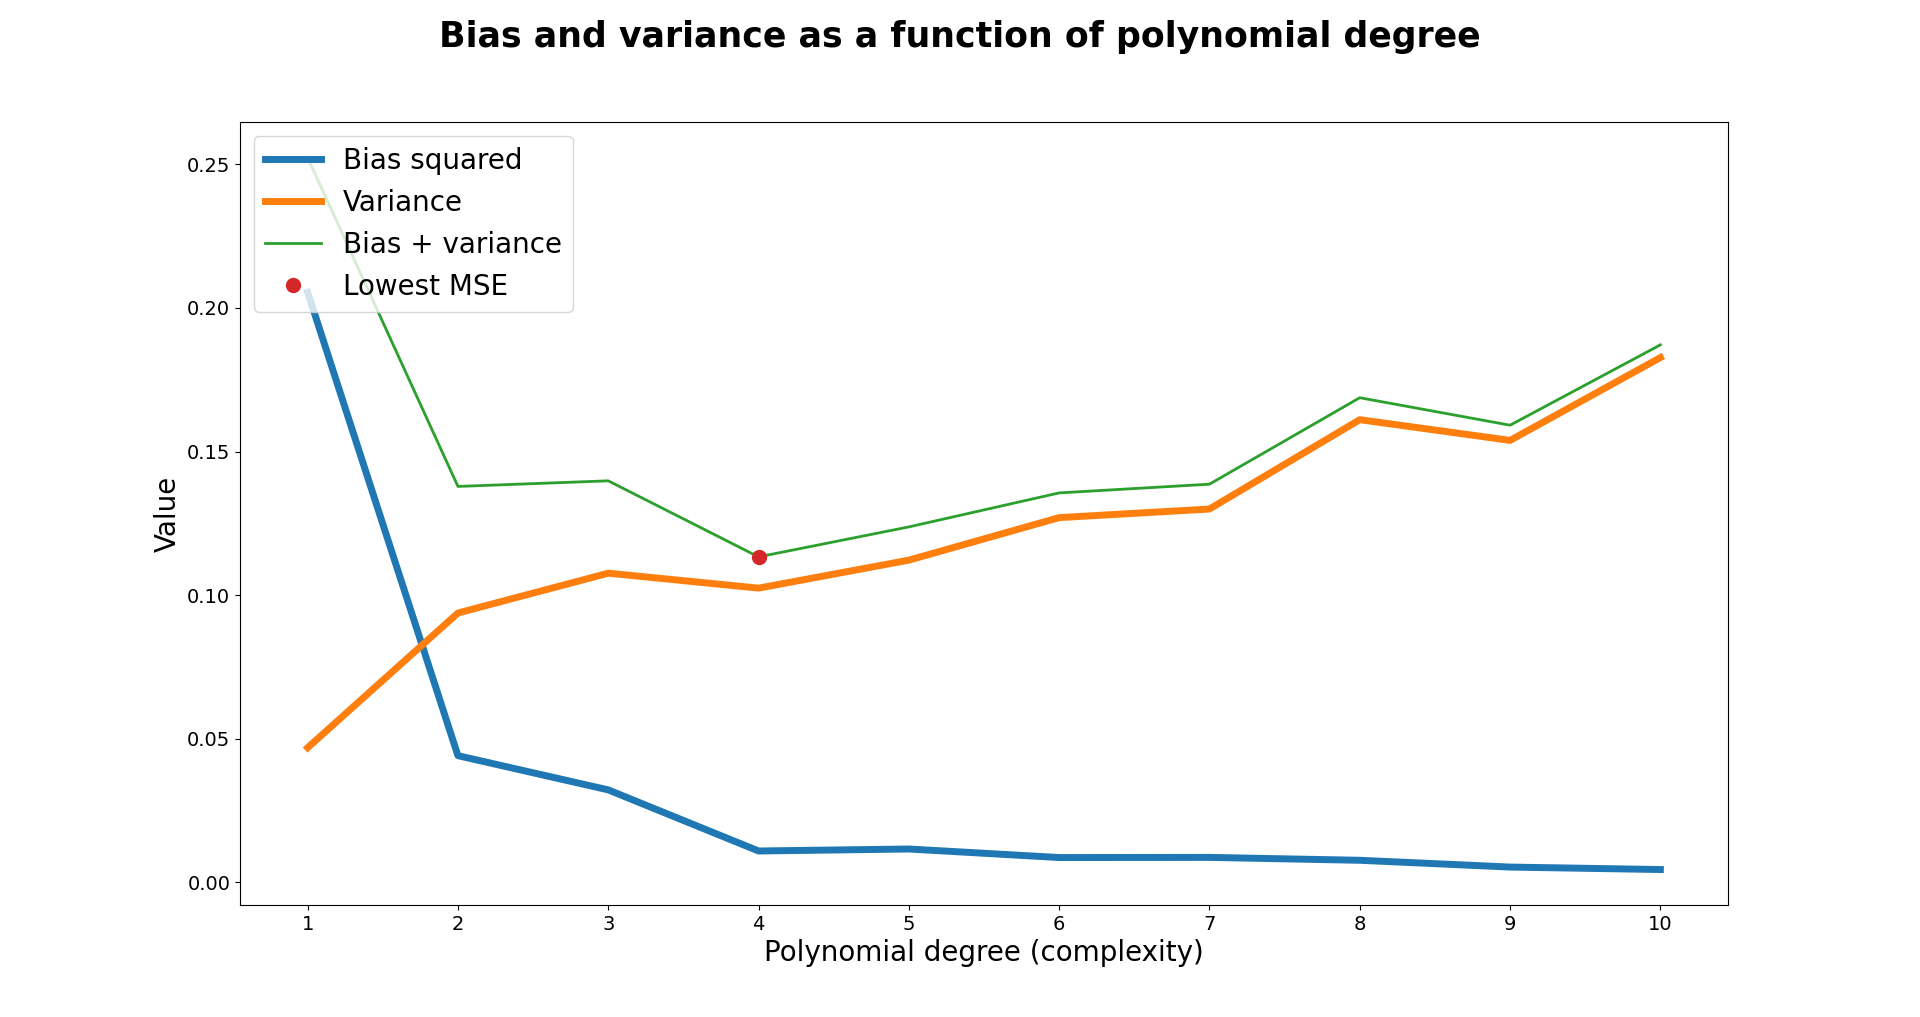
\includegraphics[width = 1\linewidth]{C:/Users/Sander/Documents/GitHub/FYS-STK4155/Project1/Report/Figures/BVplotCV_n100_p10_noise0001_CV5.PNG}
\caption{\label{fig:BVCV2} Bias and variance decomposition of figure \ref{fig:MSECV1}. The bias and variance change as a function of polynomial degree using the CV resampling method. Here we have 100 observations while we use 5-fold CV with a noise level of $0.001$.}
\end{figure}

\noindent What we observe when comparing figure \ref{fig:MSECV1} to figure \ref{fig:MSECV2} and figure \ref{fig:BVCV1} to figure \ref{fig:BVCV2} is that the bias looks the same, but the variance increases at a lower rate when using 5-fold CV rather than 10-fold CV. As a result, the MSE is lower at higher polynomials, thus decreasing the risk of overfitting. We can continue this examination by seeing what happens when we use LOOCV as in figure \ref{fig:MSECV3} and \ref{fig:BVCV3}

\begin{figure}[H]
\centering
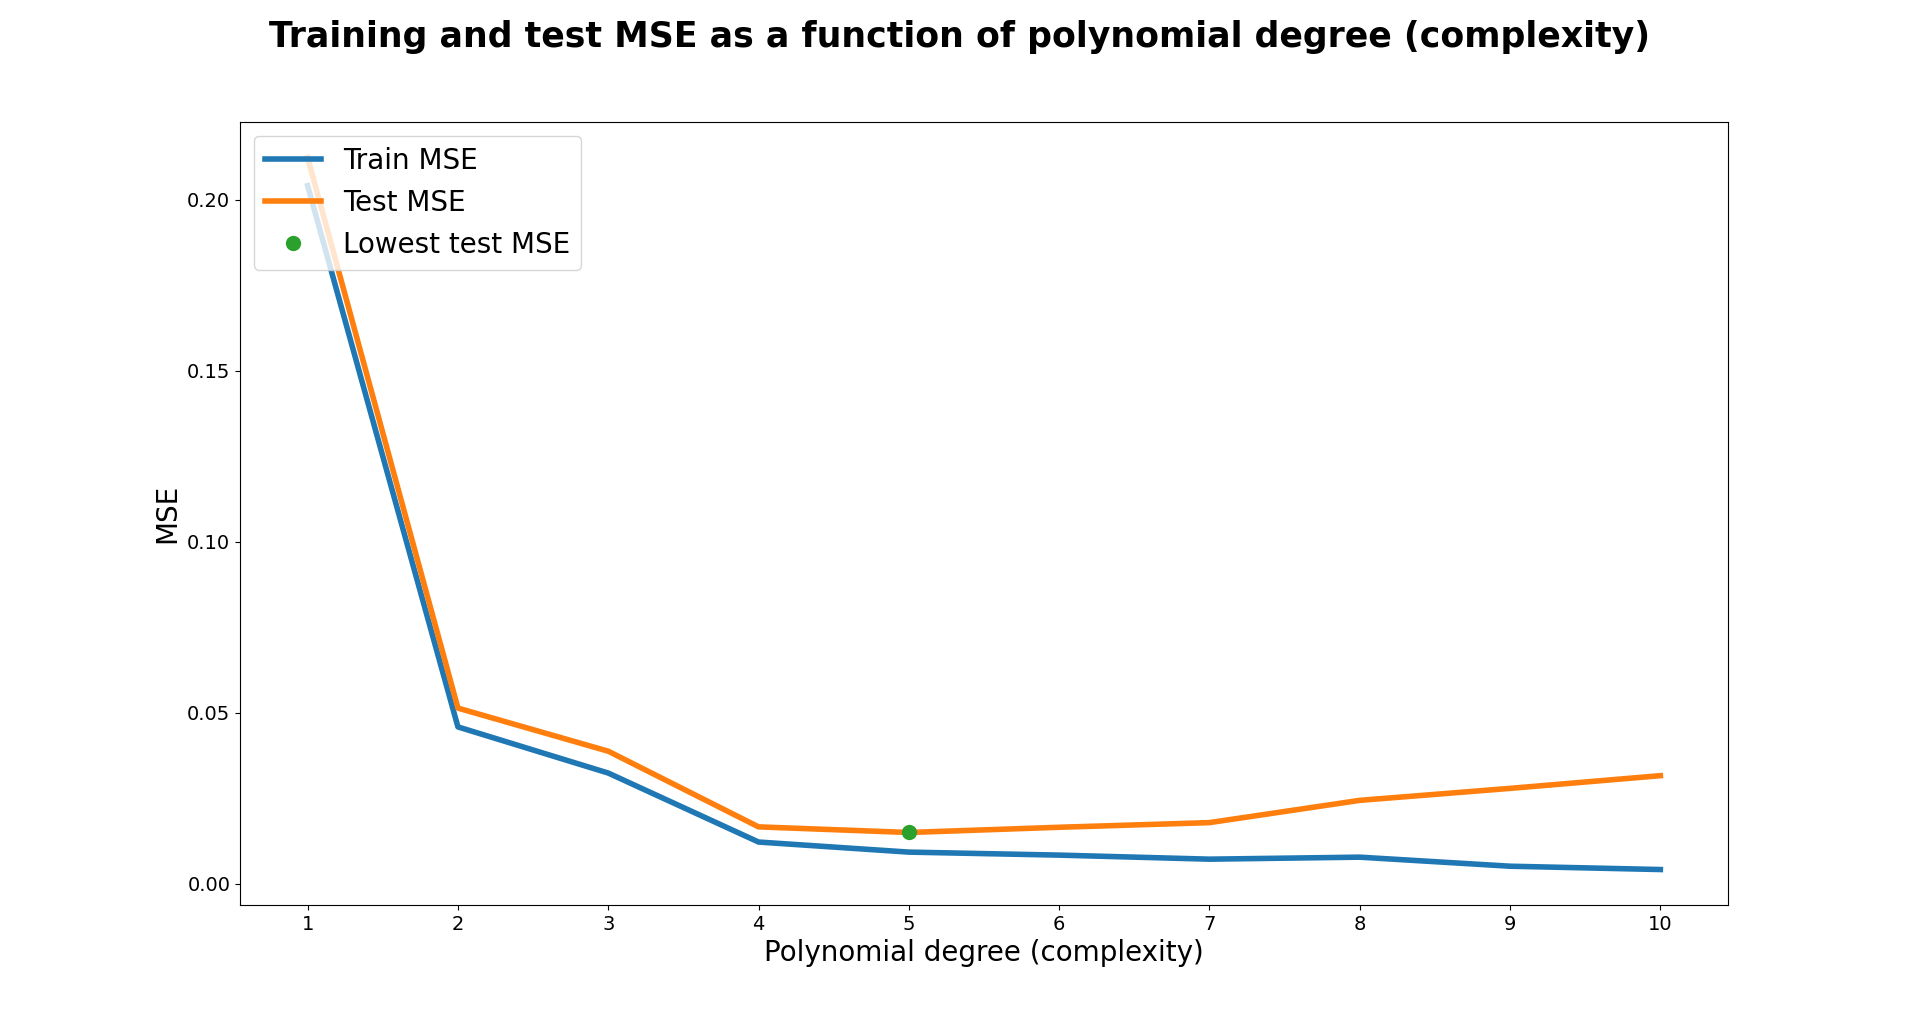
\includegraphics[width = 1\linewidth]{C:/Users/Sander/Documents/GitHub/FYS-STK4155/Project1/Report/Figures/MSECV_n100_p10_noise0001_CV1_shuffles.PNG}
\caption{\label{fig:MSECV3} MSE as a function of polynomial degree up to 10 using the cross-validation resampling method. Here we have 100 observations while we split the data into n different folds with a noise level of $0.001$.}
\end{figure}

\begin{figure}[H]
\centering
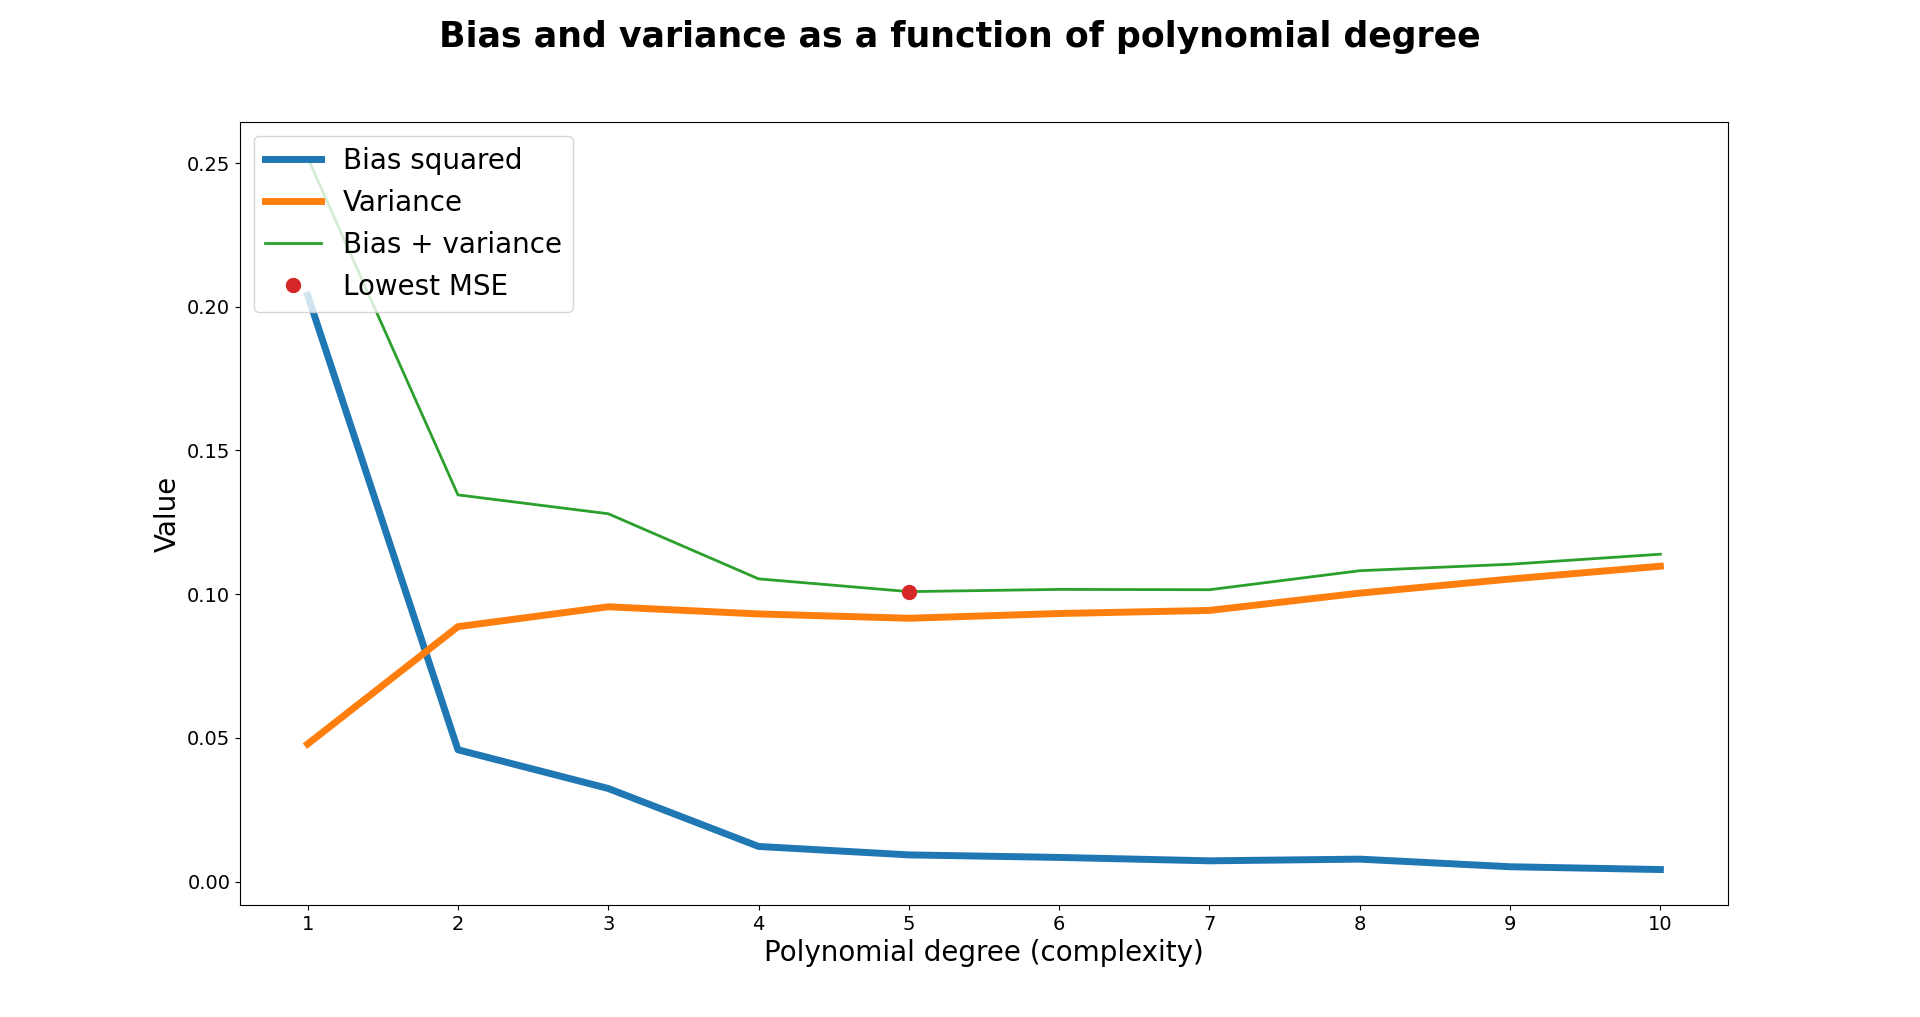
\includegraphics[width = 1\linewidth]{C:/Users/Sander/Documents/GitHub/FYS-STK4155/Project1/Report/Figures/BVplotCV_n100_p10_noise0001_CV1.PNG}
\caption{\label{fig:BVCV3} Bias and variance decomposition of figure \ref{fig:MSECV1}. The bias and variance change as a function of polynomial degree using the CV resampling method. Here we have 100 observations while we use LOOCV with a noise level of $0.001$.}
\end{figure}

\noindent Like previously discussed, the slope of the variance is less steep than that of the 10 and 5-fold CVs, and the MSE is therefore lower at higher polynomial degrees. The reason for this effect is that decreasing the fold size "creates" more data out of thin air, and having more data means that we could fit higher order polynomials without over-fitting, as previously discussed. This is observed from figures \ref{fig:MSECV3} and \ref{fig:BVCV3} as the lowest MSE is located at $p = 5$ instead of $p = 4$ as seen for higher folds. This effect could possibly also be achieved using bootstrap if we used more than 100 bootstrap samples. The two different methods seems to yield similar result which strengthen our believe in the resampling methods. This allows us to proceed to other linear regression schemes in the coming exercises.

\newpage

\noindent \textbf{d)} We have only utilized the ordinary least squares (OLS) regression scheme so far, but now we want to utilize two different shrinkage methods, namely the Ridge and Lasso regression schemes. We will start by looking at the Ridge regression scheme and then proceed to Lasso in the next exercise. 
\\
Shrinkage methods like Ridge aim to find which variables are significant and which variables are not, and then removing the influence of the in-significant variables by either setting them to zero (Lasso) or close to zero (Ridge). This is done by adding the shrinkage factor $\lambda$ to both sides of the OLS equation (equation \ref{eq:LinReg}) such that

\begin{equation}\label{eq:RidgeDerive}
\begin{aligned}
\boldsymbol{\hat{y}}_{Ridge} + \lambda |\boldsymbol{\beta}|^2 = \textbf{X}\boldsymbol{\beta} + \lambda  |\boldsymbol{\beta}|^2
\end{aligned}
\end{equation}

\noindent Solving equation \ref{eq:RidgeDerive} for the regression coefficients $\boldsymbol{\beta}$ yields

\begin{equation}\label{eq:RidgeDerive2}
\begin{aligned}
\boldsymbol{\beta} = (\textbf{X}^T \textbf{X} + \lambda \textbf{I})^{-1} \textbf{X}^T \boldsymbol{\hat{y}}_{Ridge}
\end{aligned}
\end{equation}

\noindent Where $\textbf{I}$ is the identity matrix. We can then repeat the analysis of exercises a through c, but this time using equation \ref{eq:RidgeDerive2} to train the data. 
\\
First let us investigate how the MLE of the Ridge regression changes as a function of different polynomial degrees. If we again repeat the exact experiment as in exercise b), that is a original data set consisting of 100 observations, a noise level of $0.001$, a train/test split of $75/25$ and with 100 bootstrap iterations we obtain figure \ref{fig:MSERidgeBoot3}

\begin{figure}[H]
\centering
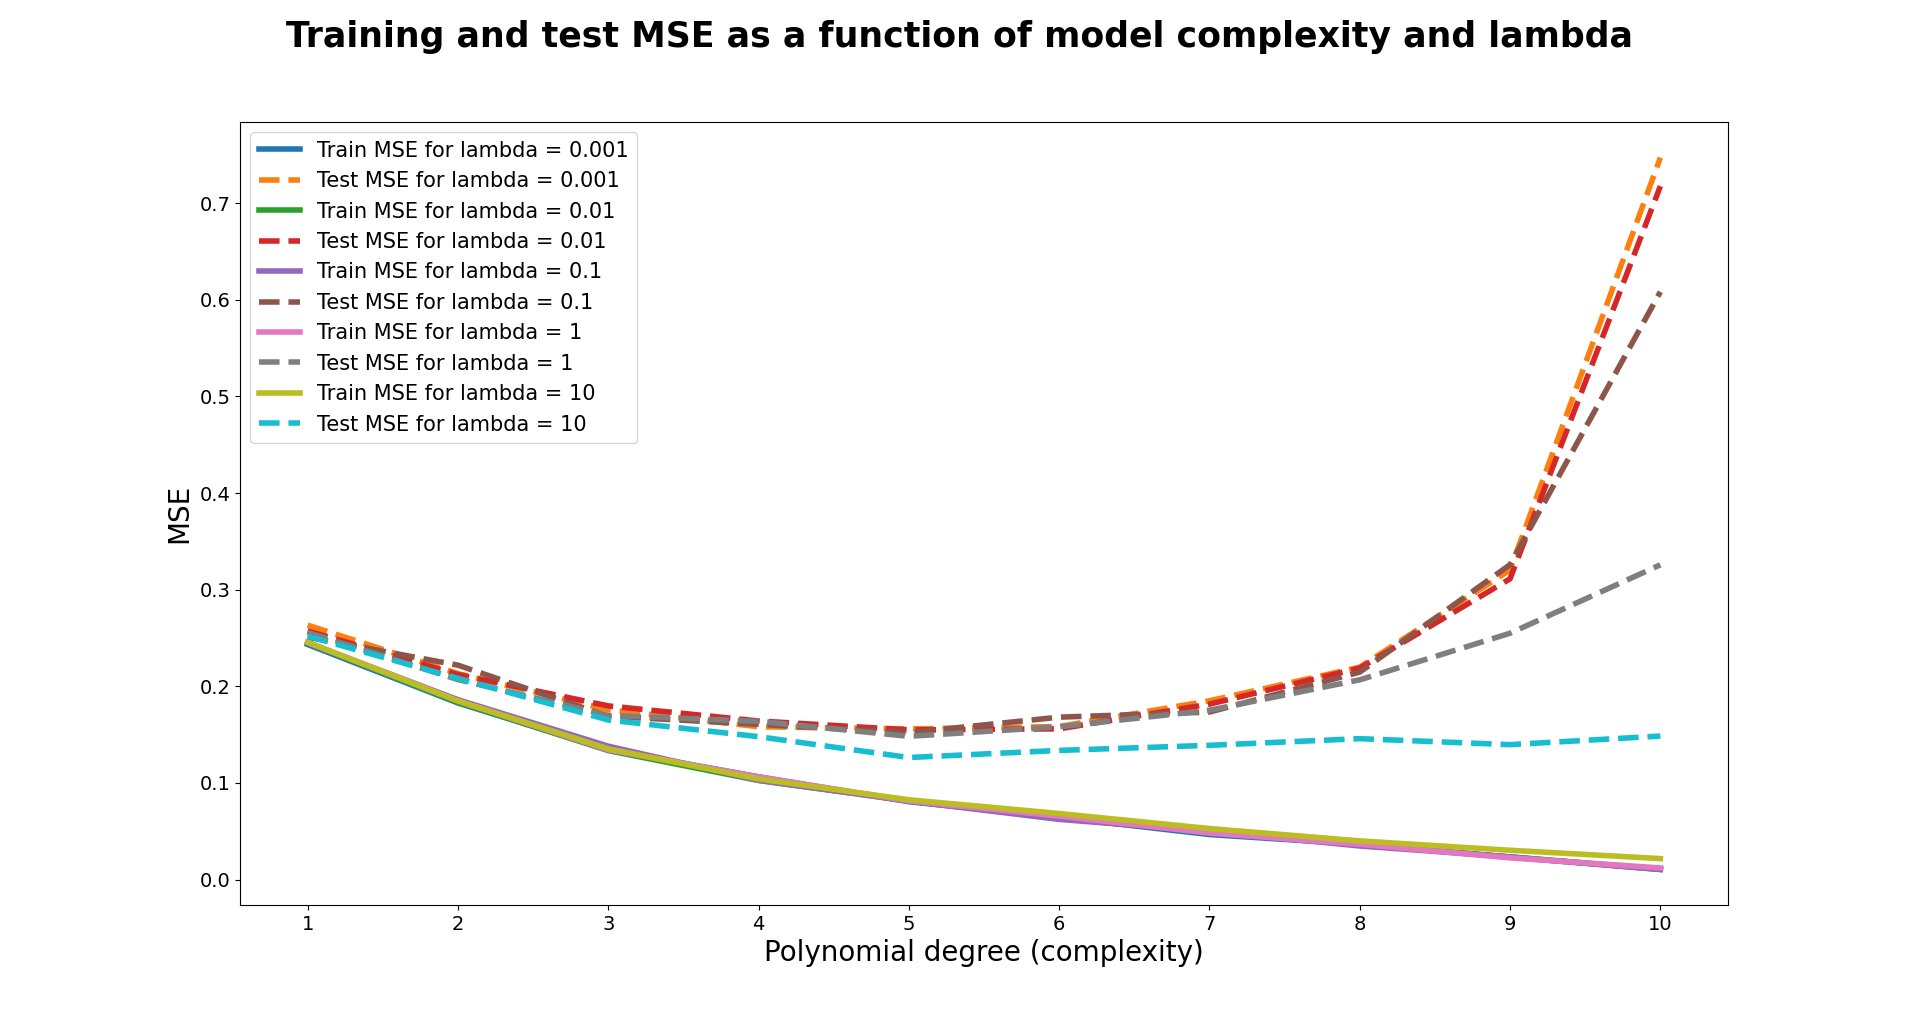
\includegraphics[width = 1\linewidth]{C:/Users/Sander/Documents/GitHub/FYS-STK4155/Project1/Report/Figures/MSEBOOT_n100_p10_noise0001_B100_RIDGE.PNG}
\caption{\label{fig:MSERidgeBoot3} MSE as a function of polynomial degree up to 10 for different values of $\lambda$ using the bootstrap resampling method with 100 iterations. Here we have 100 observations while we split the data into $75/25$ train/test split with a noise level of $0.001$.}
\end{figure}

\noindent It can be observed from figure \ref{fig:MSERidgeBoot3} that the training MSE goes towards zero regardless of the $\lambda$-value. The test MSE initially decreases to some value of p, but will eventually start to increase. The increase seems to be dependent on the value of $\lambda$, as lower values seem to increase faster than the higher values of $\lambda$. We can observe that the test MSE for $\lambda = 10$ never seems to increase, while the test MSE for $\lambda = 0.001$ seems to increase drastically after $p = 5$. Again, it seems that $p = 5$ is the polynomial degree of minimum MSE. We can decompose figure \ref{fig:MSERidgeBoot3} into its bias and variance components as done in figure \ref{fig:BVRidge1}

\begin{figure}[H]
\centering
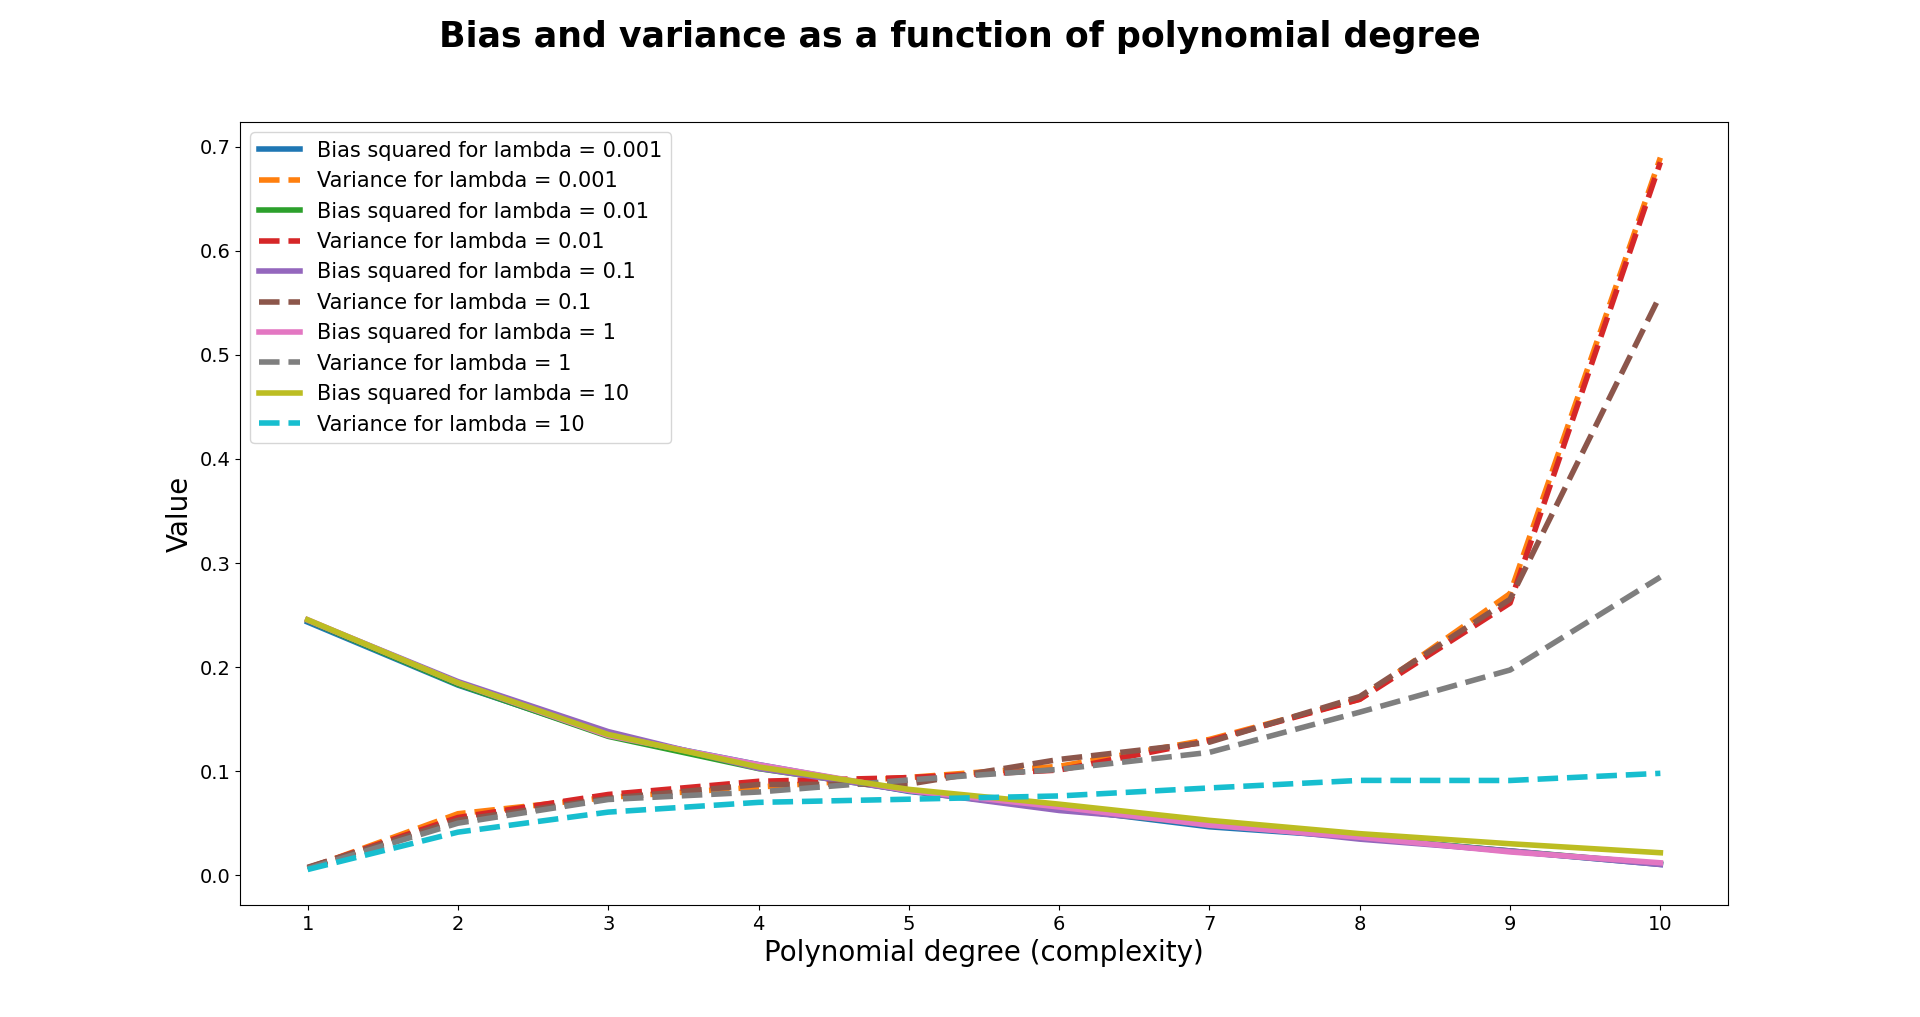
\includegraphics[width = 1\linewidth]{C:/Users/Sander/Documents/GitHub/FYS-STK4155/Project1/Report/Figures/BVplotBOOT_n100_p10_noise0001_ts025_B100_RIDGE.PNG}
\caption{\label{fig:BVRidge1} Bias and variance decomposition of figure \ref{fig:MSERidgeBoot3}. The bias and variance change as a function of polynomial degree and values of $\lambda$ using the bootstrap resampling method. Here we have 100 observations while we use a $75/25$ train/test split with a noise level of $0.001$.}
\end{figure}

\noindent We can observe from figure \ref{fig:BVRidge1} that the bias always decreases as previously seen in exercise b) (figure \ref{fig:BVBOOT1}). However, the variance seem to depend on both the complexity of our model and the value of $\lambda$. Figure \ref{fig:BVRidge1} confirms what we previously saw in figure \ref{fig:MSERidgeBoot3}, namely that higher values of $\lambda$ yields higher variance as a function of complexity, thus yielding a higher MSE.
\\
The next step is to see what happens with the beta coefficients when we apply different values of $\lambda$ to equation \ref{eq:RidgeDerive2}. We can plot the regression coefficient values for a given range of polynomial degrees and see how the value changes. Here we have chosen polynomials up to degree 5 a this is where the point of lowest MSE i located and we have chosen $\lambda$-values as $[0.00001, 0.0001, 0.001, 0.01, 0.1, 1, 10, 100, 1000, 10000, 100000]$. The result is plotted in figure \ref{fig:LambdaPlot1}

\begin{figure}[H]
\centering
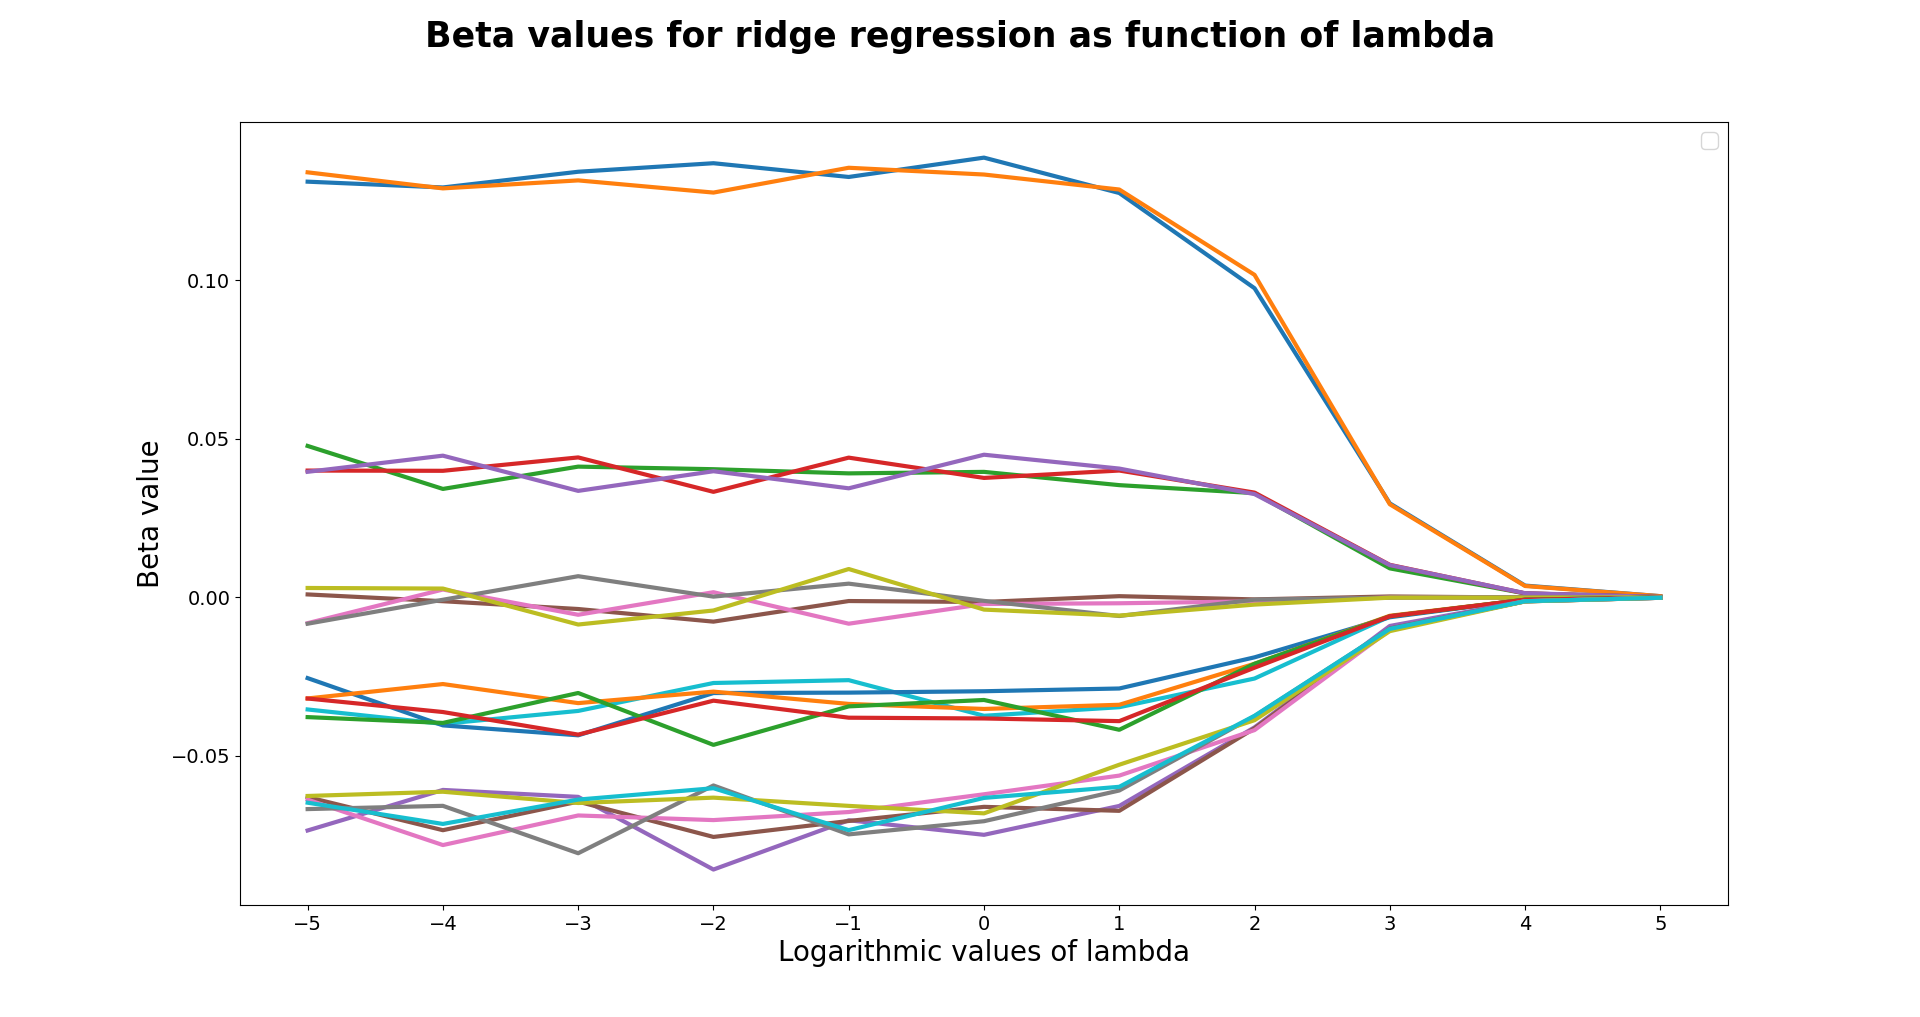
\includegraphics[width = 1\linewidth]{C:/Users/Sander/Documents/GitHub/FYS-STK4155/Project1/Report/Figures/LambdaPlot_n100_p5_noise0001_ts025_B100_RIDGE.PNG}
\caption{\label{fig:LambdaPlot1} Regression coefficient values of up to $p = 5$ as function of logarithmic $\lambda$-value using the bootstrap method with 100 iterations. The original dataset is of size 100.}
\end{figure}

\noindent It is difficult to see any trends as we have so many regression coefficients and we therefore categorize the plot into polynomial degree such that first order polynomials ($x,y$) have one color and second order polynomial ($xy,x^2,y^2$) have another color and so on. The resulting plot is shown in figure \ref{fig:LambdaPlot2}

\begin{figure}[H]
\centering
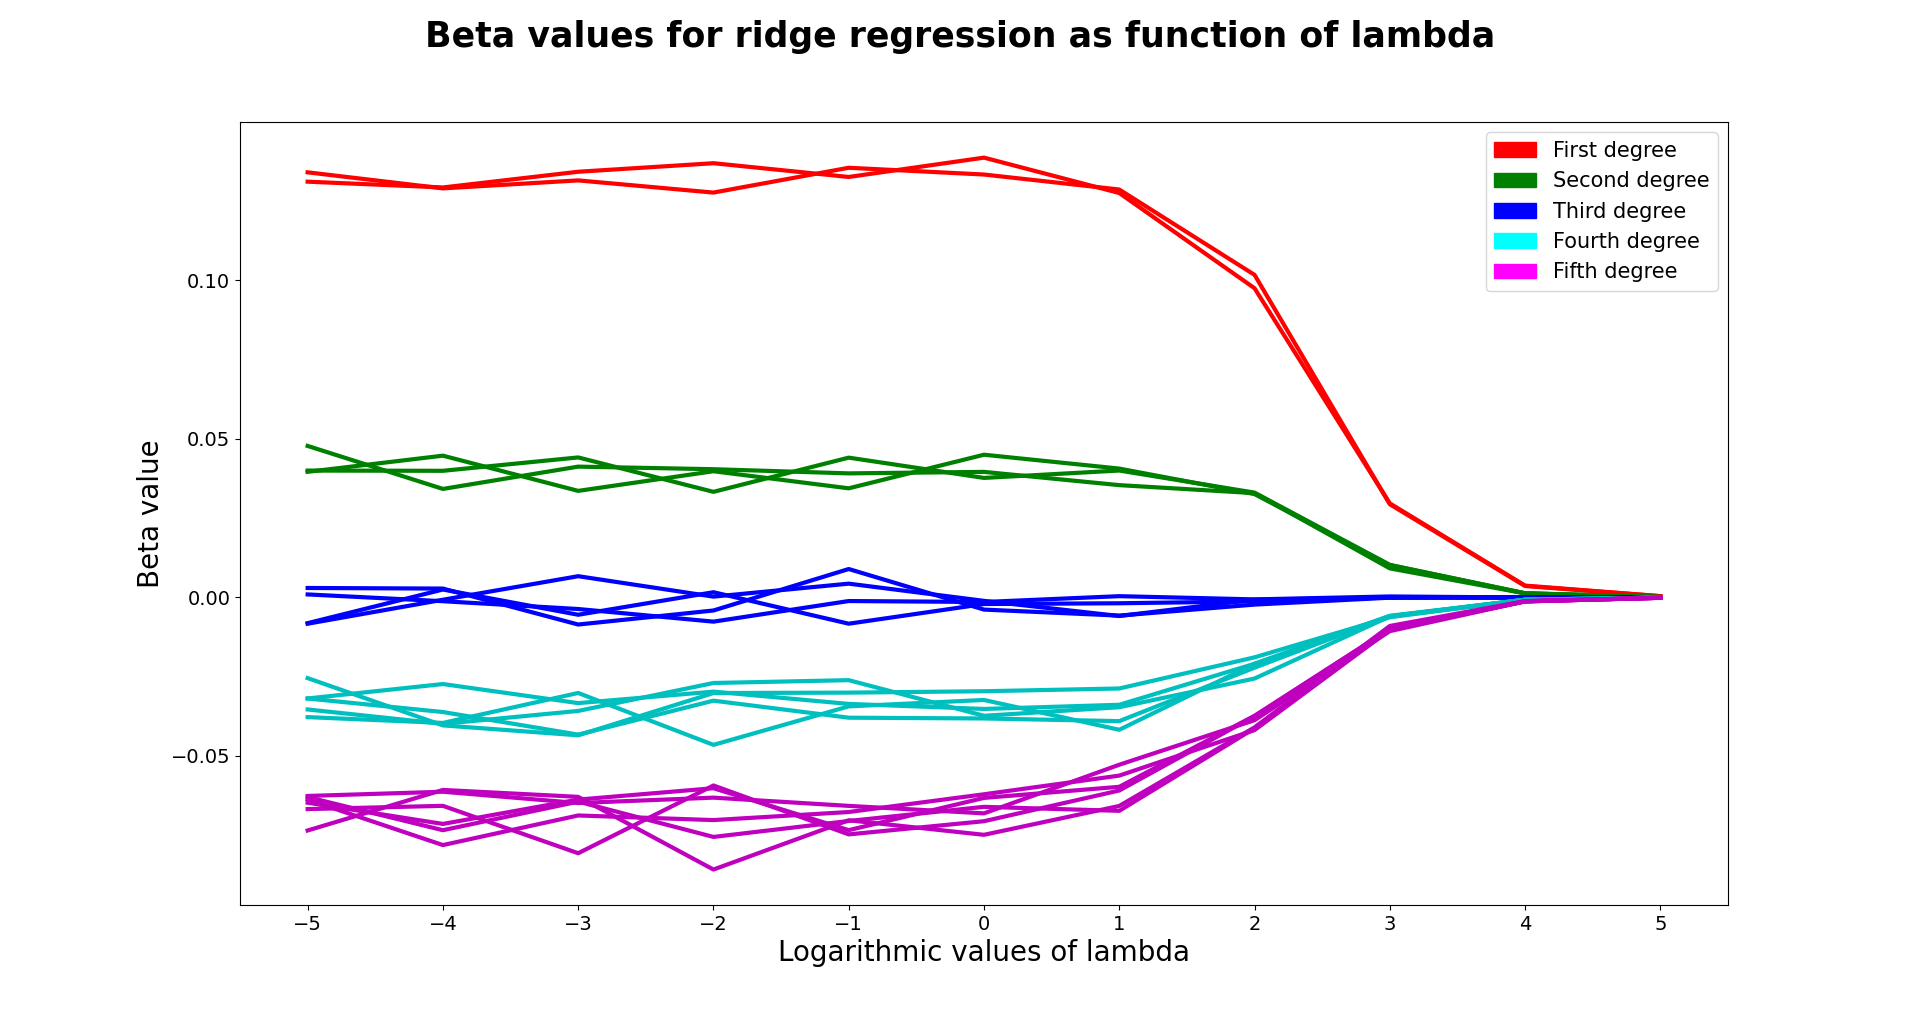
\includegraphics[width = 1\linewidth]{C:/Users/Sander/Documents/GitHub/FYS-STK4155/Project1/Report/Figures/LambdaPlot_n100_p5_noise0001_ts025_B100_RIDGESort.PNG}
\caption{\label{fig:LambdaPlot2} Regression coefficient values of up to $p = 5$ as function of logarithmic $\lambda$-value using the bootstrap method with 100 iterations. The original dataset is of size 100. Here we have sorted polynomials of the same degree into the same color}
\end{figure}

\noindent From figure \ref{fig:LambdaPlot2} we can observe that the Ridge regression treats different polynomial degree unevenly. Much of the point of the ridge regression is to reduce the the variables in the design matrix towards zero, depending on their statistical significance. The higher the $\lambda$-values, the more variables will be reduced towards zero, but not exactly zero. We can observe this by comparing the third and first degree polynomial in figure \ref{fig:LambdaPlot2}. The third degree polynomial is reduced to a value close to zero at around $10^{-2} = 0.1$, while the first degree polynomial does not approach zero before $10^2 = 100$. This means that the ridge regression algorithm deems third degree polynomials as less significant than that of the first order polynomials. We can extend this though process and see that all variables will be reduced closed to zero (regardless of their polynomial degree) if $\lambda$ is large enough.
\\
Let us now explore the CV resampling approach. We implement the CV algorithm the same way as in exercise c) and we see investigate how the MSE changes as function of model complexity. We will use the exact same parameters as previously with $n = 100$ observations in the original data set, a noise-level of $0.001$ and 10 polynomial degrees. Furthermore, we want to try the 10-fold, 5-fold and leave-one-out cross-validations and see what the difference between the outcomes are. The MSE versus polynomial degree is plotted for each CV-type in figure \ref{fig:MSERidgeCV1}, \ref{fig:MSERidgeCV2} and \ref{fig:MSERidgeCV3}

\begin{figure}[H]
\centering
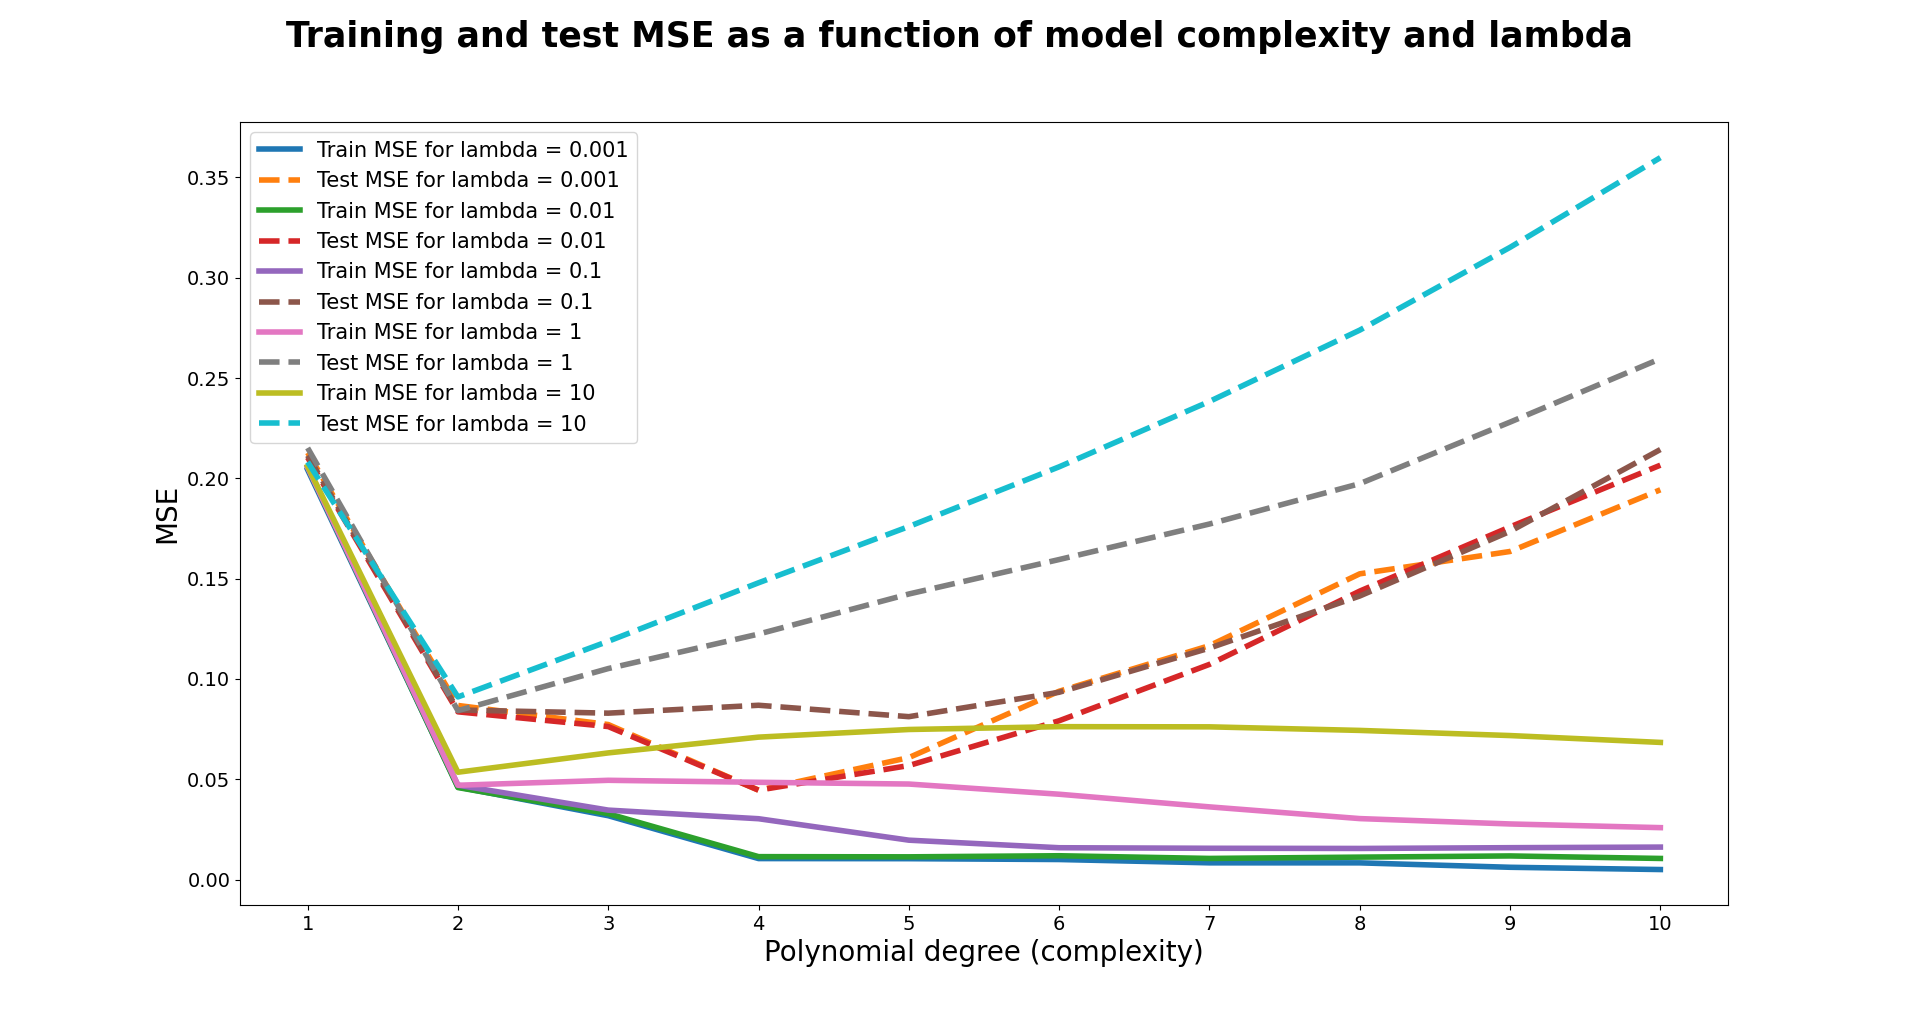
\includegraphics[width = 1\linewidth]{C:/Users/Sander/Documents/GitHub/FYS-STK4155/Project1/Report/Figures/MSECV_n100_p10_noise0001_CV10_RIDGE.PNG}
\caption{\label{fig:MSERidgeCV1} MSE as a function of polynomial degree up to 10 for different values of $\lambda$ using the 10-fold CV resampling method. Here we have 100 observations while we consider every possible permutation of a 10-fold cross-validation with a noise level of $0.001$.}
\end{figure}

\begin{figure}[H]
\centering
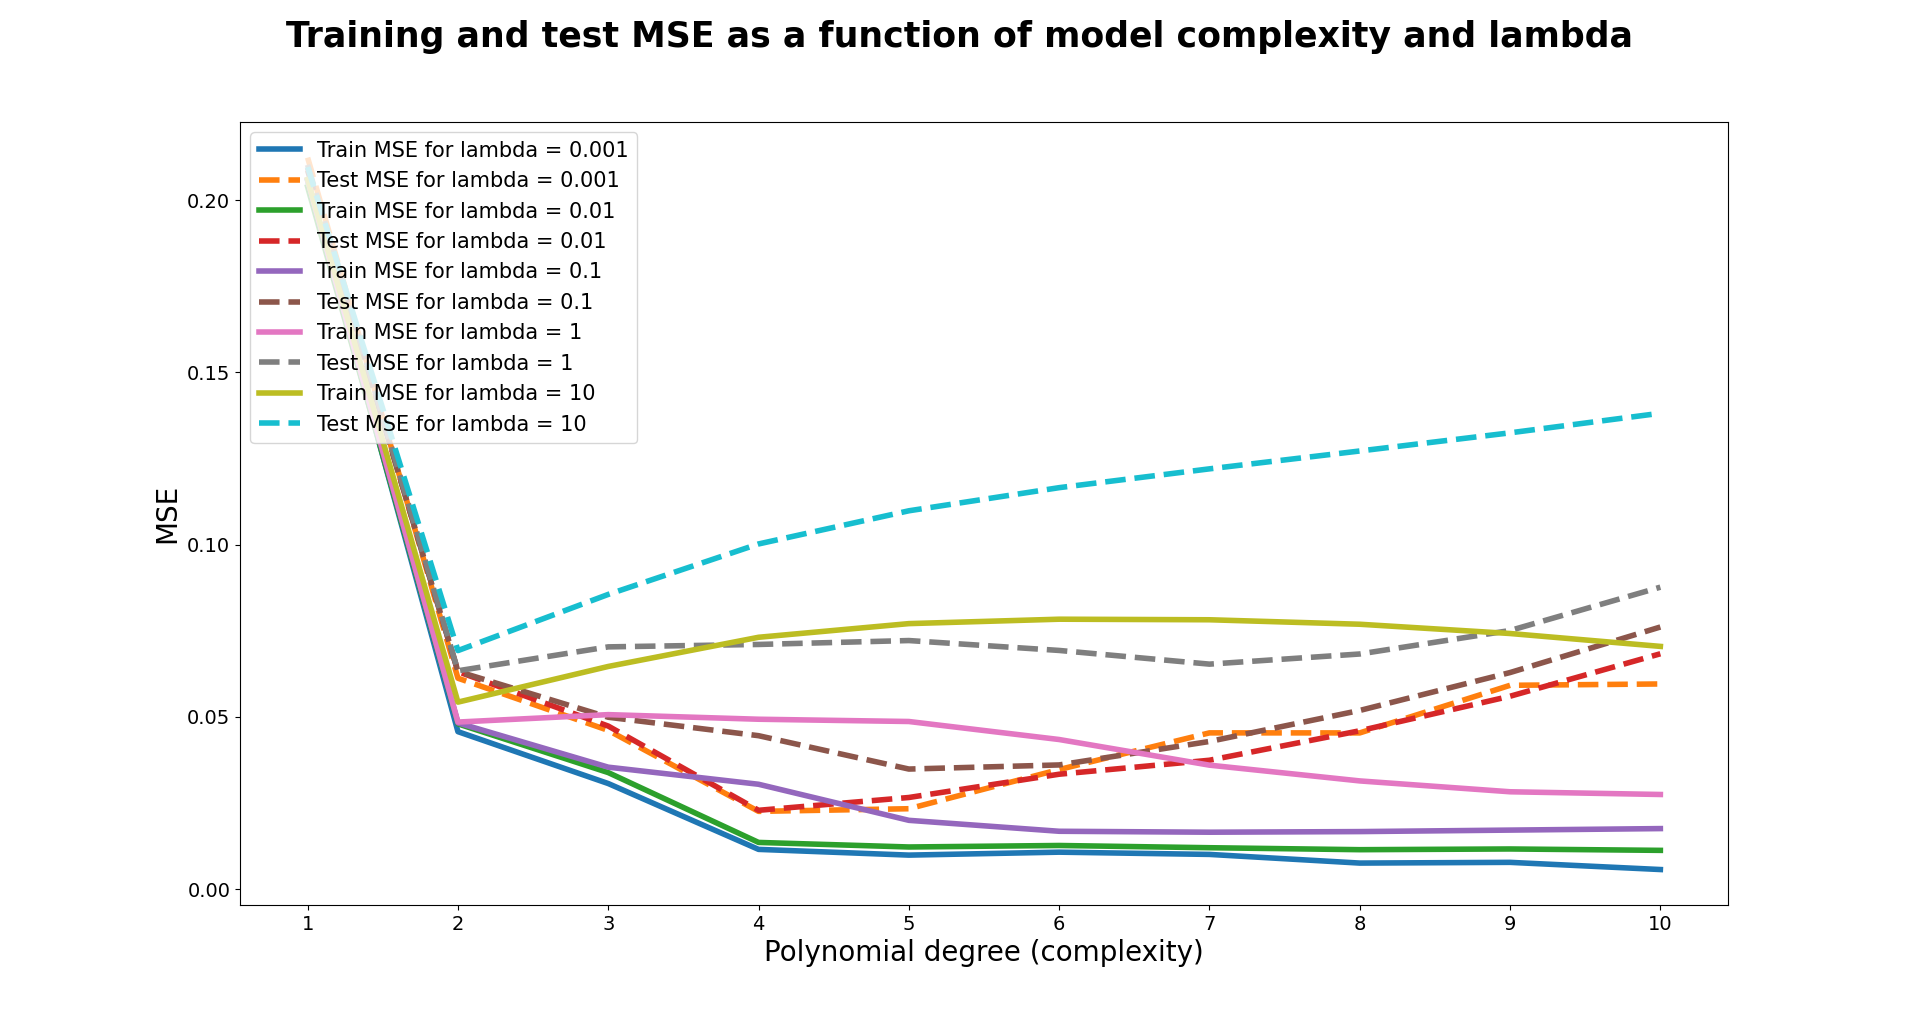
\includegraphics[width = 1\linewidth]{C:/Users/Sander/Documents/GitHub/FYS-STK4155/Project1/Report/Figures/MSECV_n100_p10_noise0001_CV5_RIDGE.PNG}
\caption{\label{fig:MSERidgeCV2} MSE as a function of polynomial degree up to 10 for different values of $\lambda$ using the 5-fold CV resampling method. Here we have 100 observations while we consider every possible permutation of a 5-fold cross-validation with a noise level of $0.001$.}
\end{figure}

\begin{figure}[H]
\centering
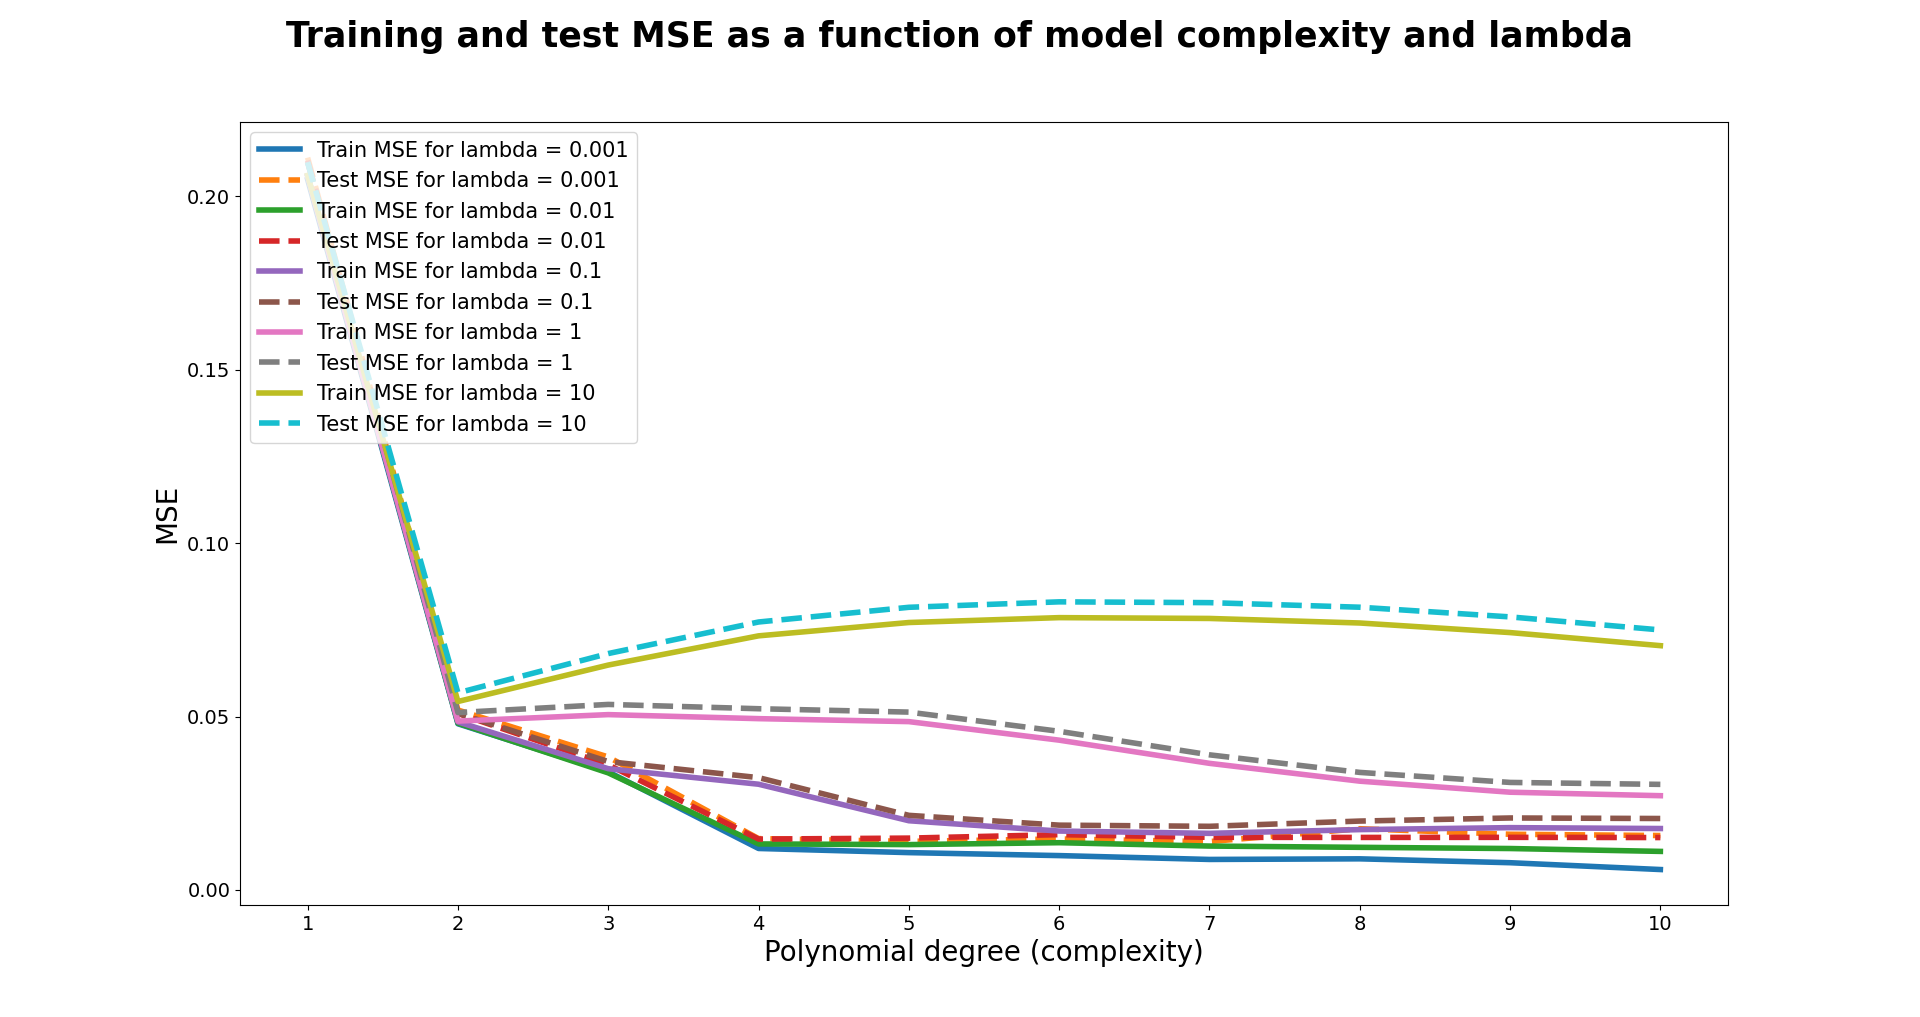
\includegraphics[width = 1\linewidth]{C:/Users/Sander/Documents/GitHub/FYS-STK4155/Project1/Report/Figures/MSECV_n100_p10_noise0001_CV1_RIDGE.PNG}
\caption{\label{fig:MSERidgeCV3} MSE as a function of polynomial degree up to 10 for different values of $\lambda$ using the leave-one-out CV resampling method. Here we have 100 observations while we consider every possible permutation of a leave-one-out cross-validation with a noise level of $0.001$.}
\end{figure}

\noindent One can observe from figures \ref{fig:MSERidgeCV1}, \ref{fig:MSERidgeCV2} and \ref{fig:MSERidgeCV3} that the MSEs rapidly decrease from 1 to 2 polynomial degrees. After $p = 2$ however, some models increase in MSE while others decrease. The overall trend regardless of fold-size is that models with a high value of $\lambda$ tend to have a steeper increase in MSE. On the contrary, we see models with low values of $\lambda$ actually further decrease in MSE after $p = 2$, namely models with $\lambda$-value lower than $0.1$. However, these models also eventually increase in MSE after $p = 5$, which still seem to be the optimal complexity for most models. 
\\
What is also observed from figures \ref{fig:MSERidgeCV1}, \ref{fig:MSERidgeCV2} and \ref{fig:MSERidgeCV3} is that the training MSE for some models, namely those of higher values of $\lambda$, do not approach zero imminently. This is due to the Ridge regression reducing some of the variables to zero (least significant ones) which actually lowers the MSE of even the training data. This was not a problem when we used OLS or bootstrap resampling, meaning the CV resampling method is more sensitive to which variables are considered in the regression. 
\\
Another interesting observations is that decreasing the fold size tend to decrease the MSE. When we compare figures \ref{fig:MSERidgeCV1}, \ref{fig:MSERidgeCV2} and \ref{fig:MSERidgeCV3} we see that the LOOCV has the lowest overall MSE while the 10-fold CV has the highest overall CV. This is not surprising as using smaller folds sizes inherently "creates" more data, allowing for larger polynomial degrees to yield lower MSEs. In fact, we can see that for the LOOCV case (figure \ref{fig:MSERidgeCV3}), some of the models never really increase their test MSE for polynomials up to 10th order. This means that creating $n^2$ amount of data allows us to create models with much higher order of polynomials. This means that we can more accurately predict responses by using higher order polynomials in our model.
\\
We can decompose the test MSEs from figures \ref{fig:MSERidgeCV1}, \ref{fig:MSERidgeCV2} and \ref{fig:MSERidgeCV3} into their bias and variance components as done in figures \ref{fig:BVRidgeCV1}, \ref{fig:BVRidgeCV2} and \ref{fig:BVRidgeCV3}

\begin{figure}[H]
\centering
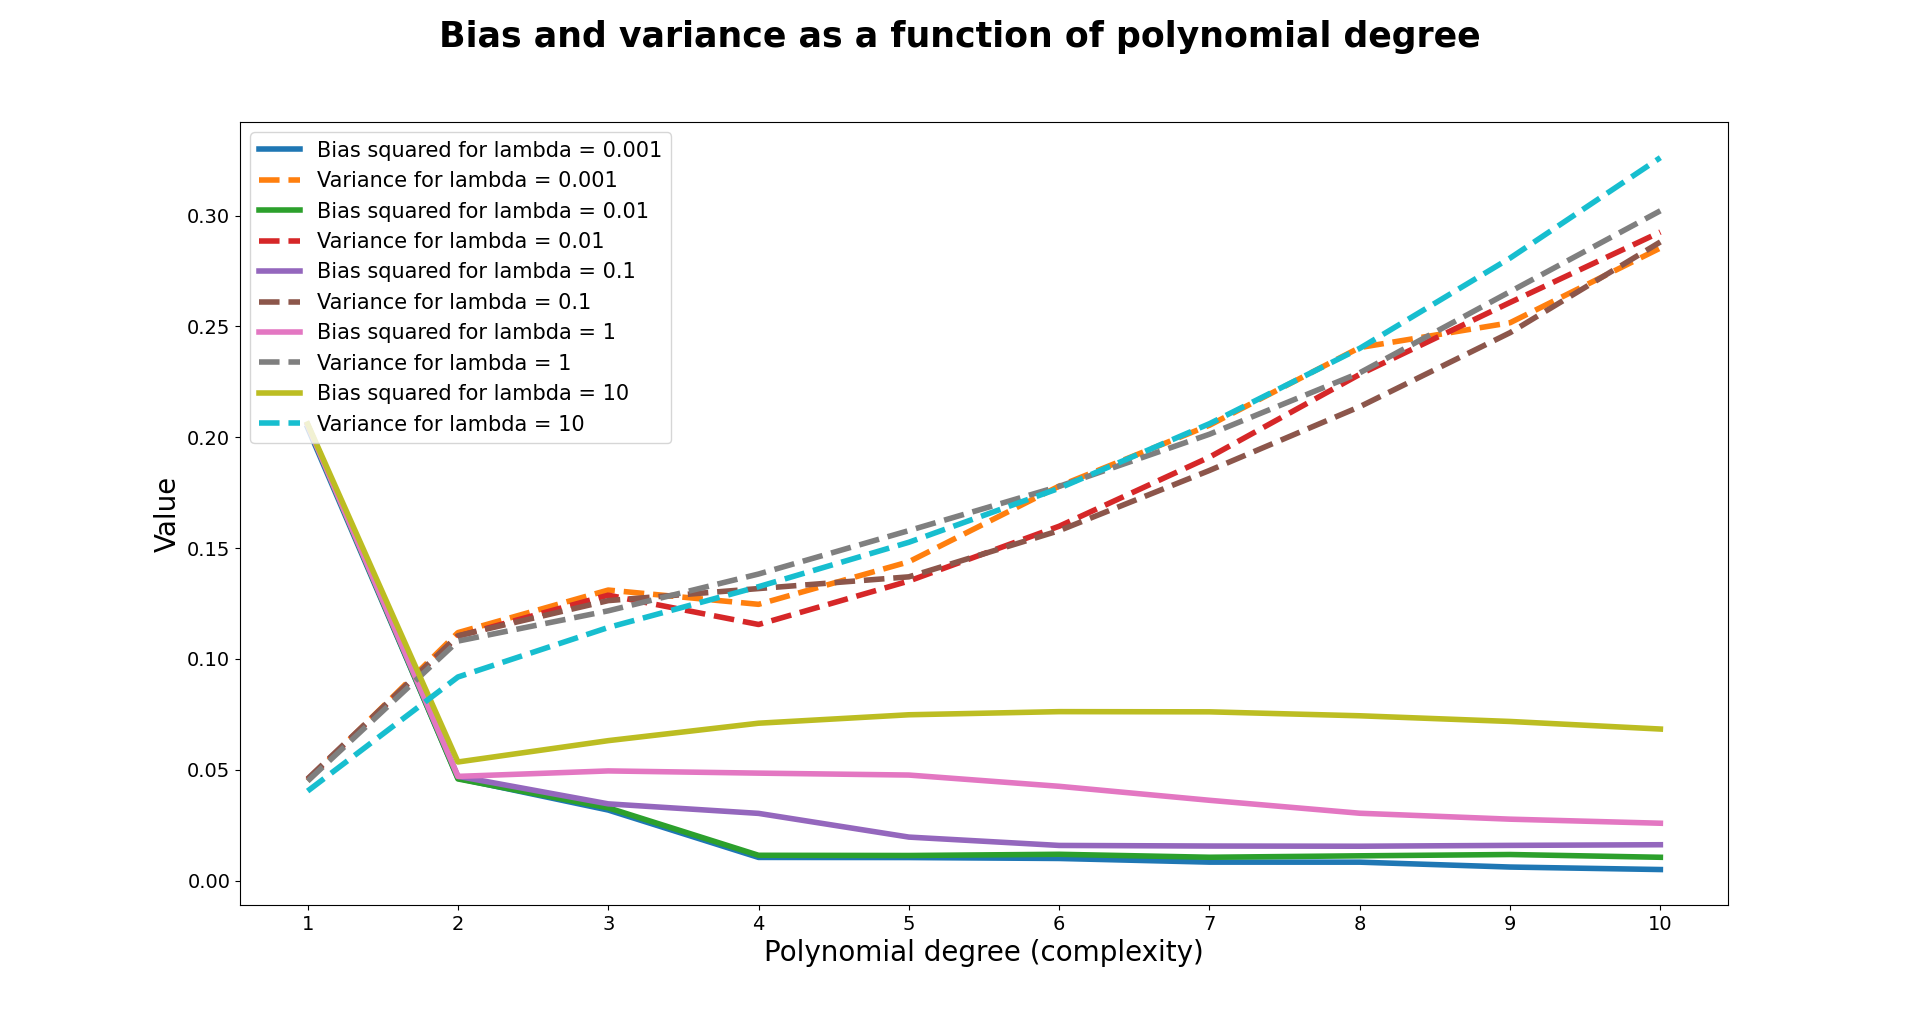
\includegraphics[width = 1\linewidth]{C:/Users/Sander/Documents/GitHub/FYS-STK4155/Project1/Report/Figures/BVplotCV_n100_p10_noise0001_CV10_RIDGE.PNG}
\caption{\label{fig:BVRidgeCV1} Bias and variance decomposition of figure \ref{fig:MSERidgeCV1}. The bias and variance change as a function of polynomial degree and values of $\lambda$ using the 10-fold CV resampling method. Here we have 100 observations with a noise level of $0.001$.}
\end{figure}

\begin{figure}[H]
\centering
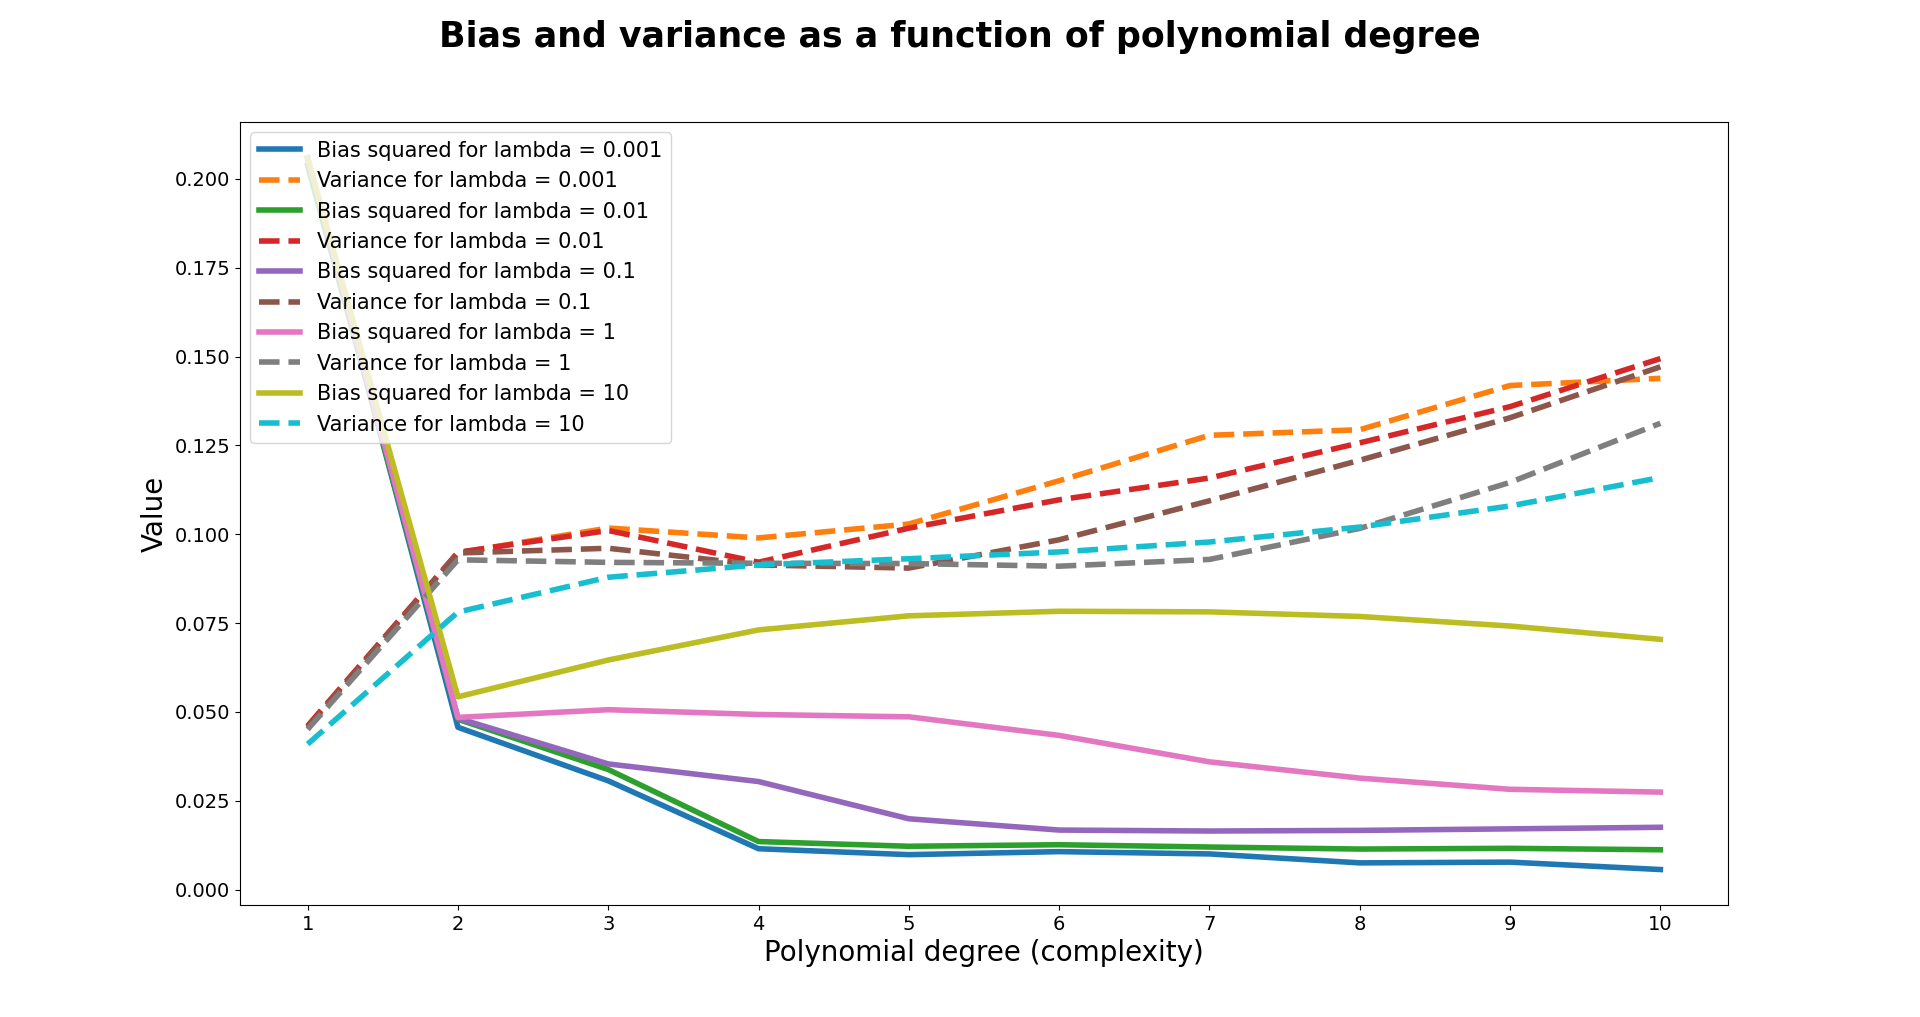
\includegraphics[width = 1\linewidth]{C:/Users/Sander/Documents/GitHub/FYS-STK4155/Project1/Report/Figures/BVplotCV_n100_p10_noise0001_CV5_RIDGE.PNG}
\caption{\label{fig:BVRidgeCV2} Bias and variance decomposition of figure \ref{fig:MSERidgeCV2}. The bias and variance change as a function of polynomial degree and values of $\lambda$ using the 5-fold CV resampling method. Here we have 100 observations with a noise level of $0.001$.}
\end{figure}

\begin{figure}[H]
\centering
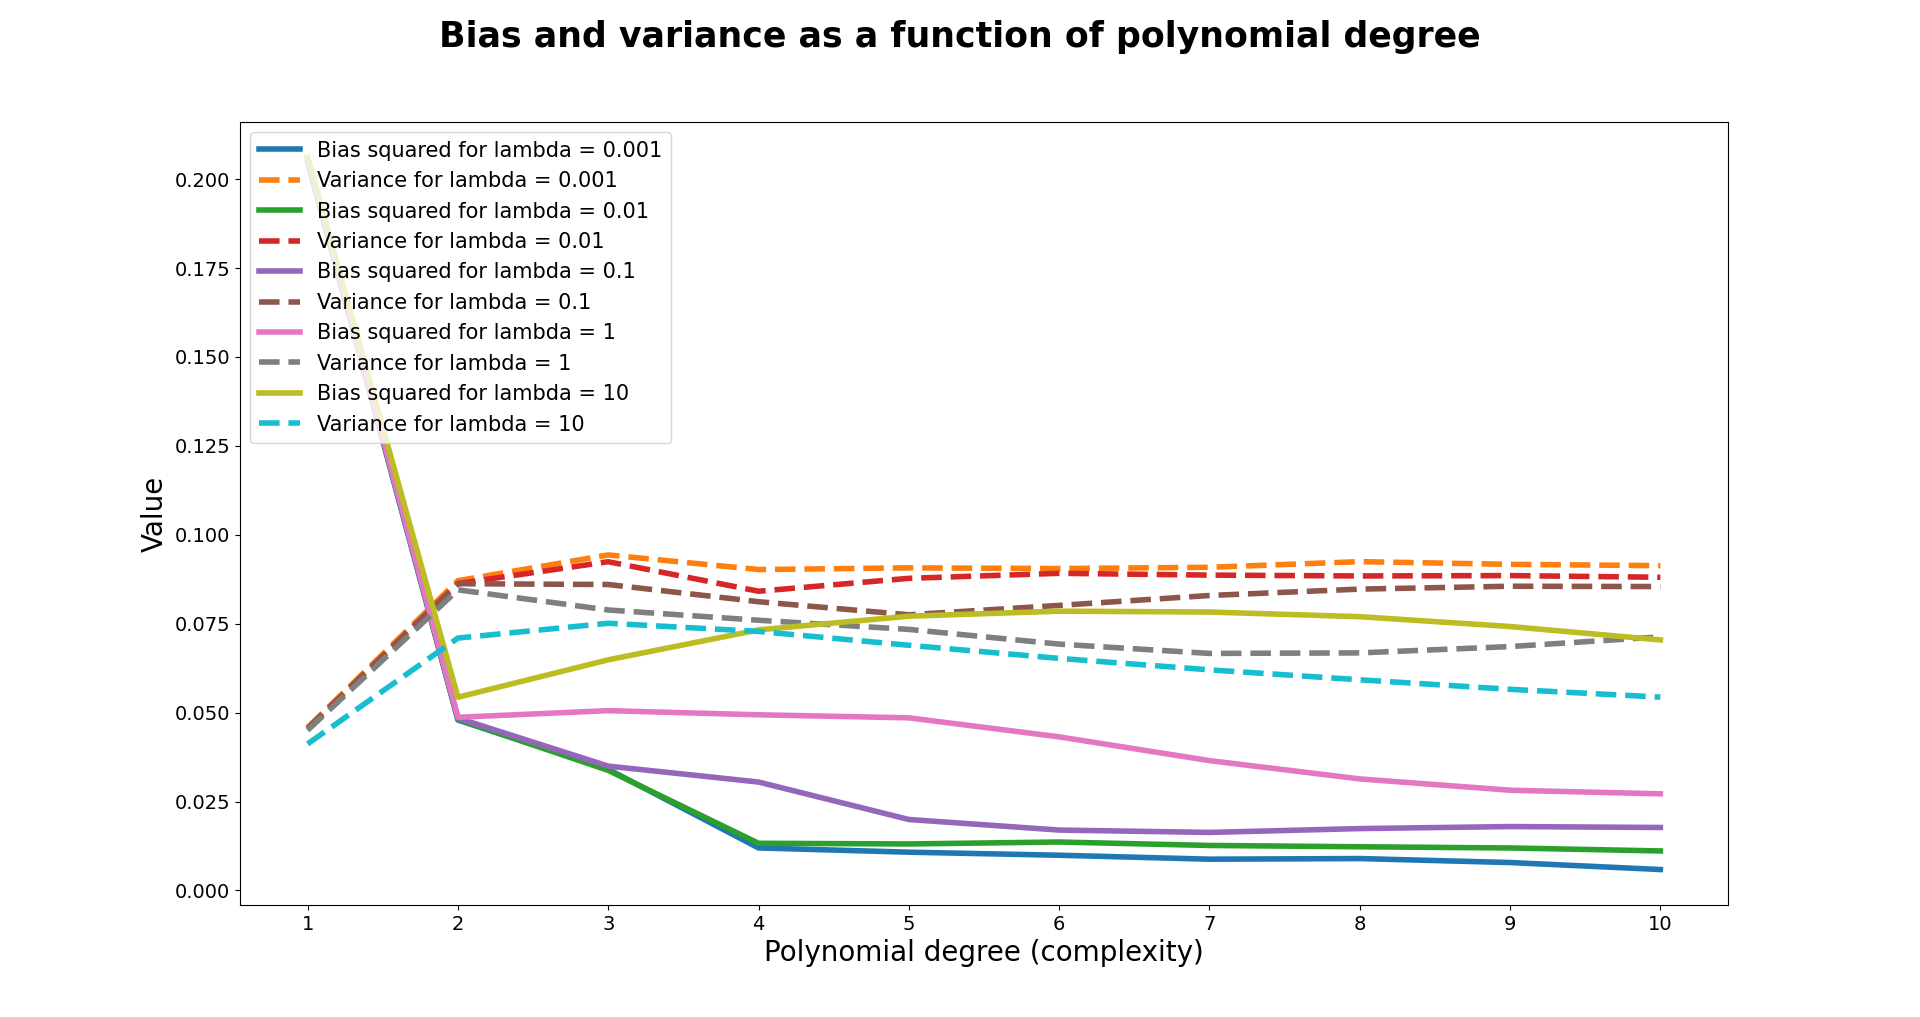
\includegraphics[width = 1\linewidth]{C:/Users/Sander/Documents/GitHub/FYS-STK4155/Project1/Report/Figures/BVplotCV_n100_p10_noise0001_CV1_RIDGE.PNG}
\caption{\label{fig:BVRidgeCV3} Bias and variance decomposition of figure \ref{fig:MSERidgeCV3}. The bias and variance change as a function of polynomial degree and values of $\lambda$ using the LOOCV resampling method. Here we have 100 observations with a noise level of $0.001$.}
\end{figure}

\noindent Figures \ref{fig:BVRidgeCV1}, \ref{fig:BVRidgeCV2} and \ref{fig:BVRidgeCV3} explains why the test MSEs decreased with smaller folds. The bias of stays the same regardless of fold-size, while the variance decreases for all values of $\lambda$. 
\\
Let us now investigate the effects of the Ridge regression on the regression coefficients. We can again plot the regression coefficient values against values of $\lambda$ for all three fold sizes as done in figure \ref{fig:LambdaPlotCV1}, \ref{fig:LambdaPlotCV2} and \ref{fig:LambdaPlotCV3}

\begin{figure}[H]
\centering
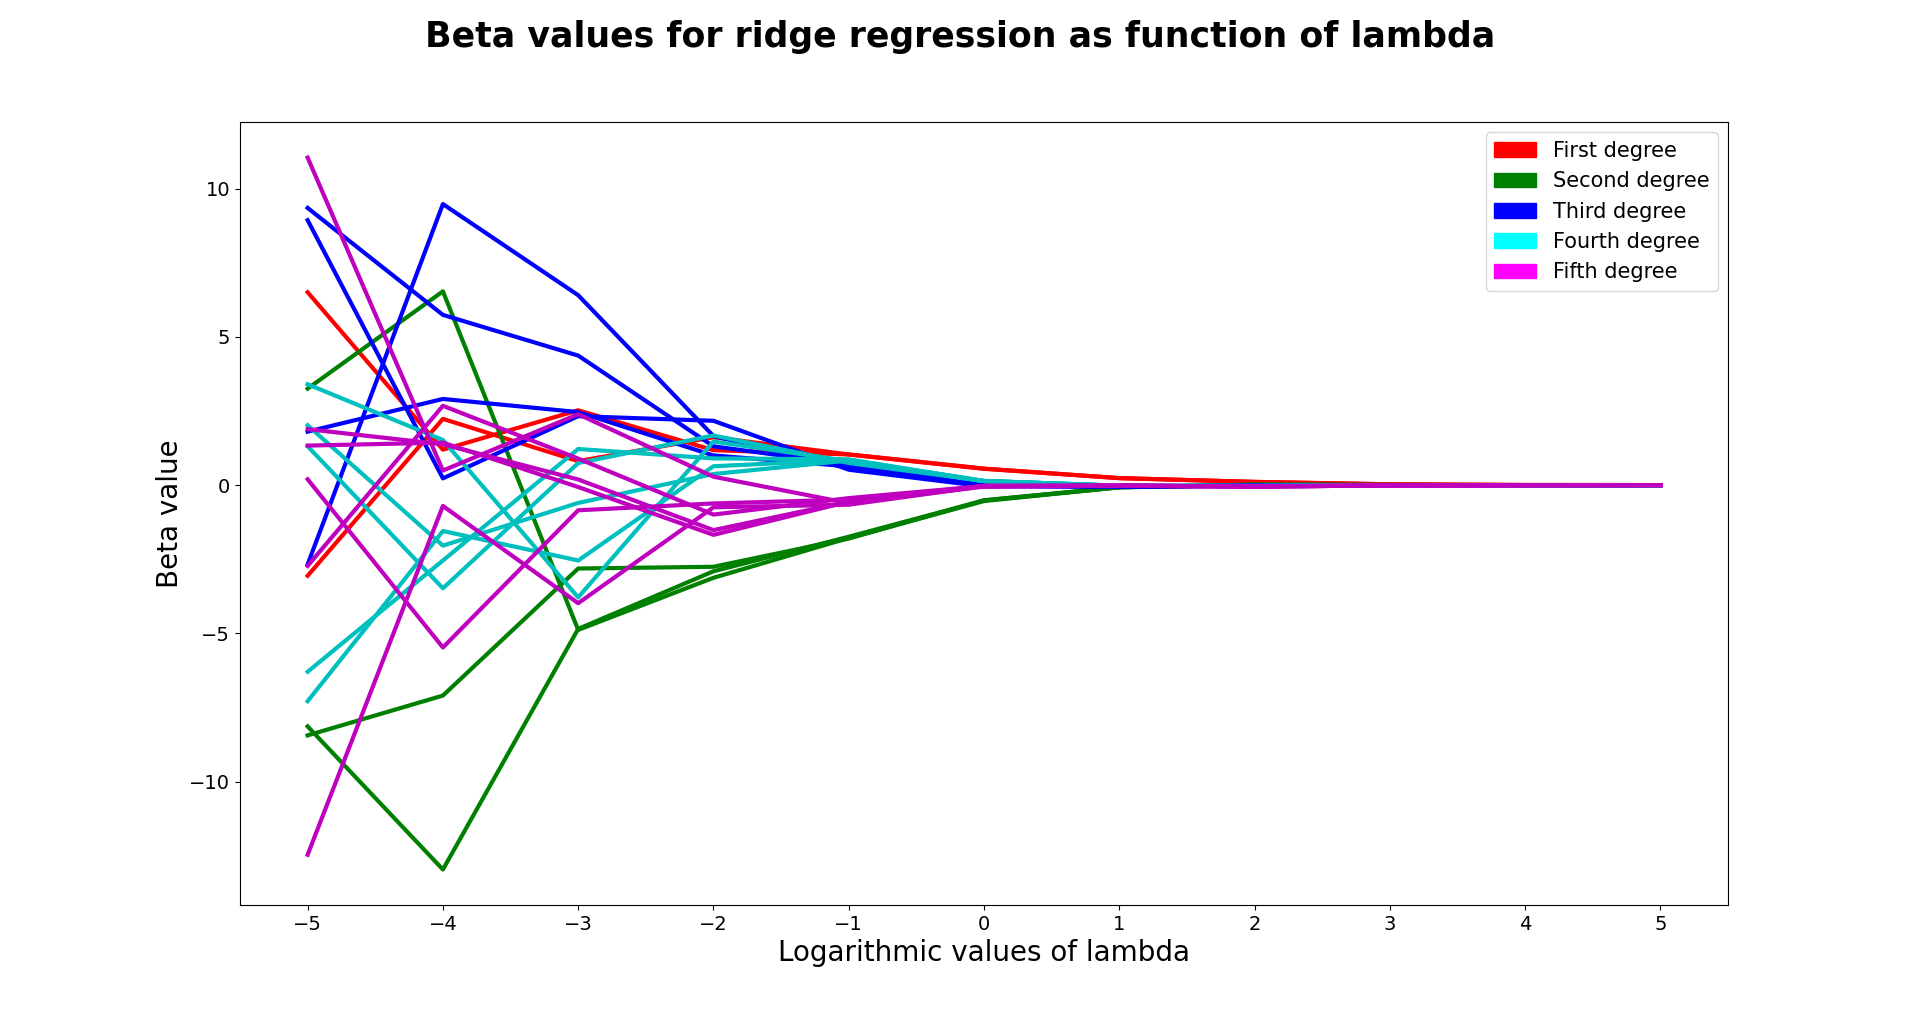
\includegraphics[width = 1\linewidth]{C:/Users/Sander/Documents/GitHub/FYS-STK4155/Project1/Report/Figures/LambdaPlot_n100_p5_noise0001_CV10_RIDGE.PNG}
\caption{\label{fig:LambdaPlotCV1} Regression coefficient values of up to $p = 5$ as function of logarithmic $\lambda$-value using the 10-fold CV method. The original dataset is of size 100. Here we have sorted polynomials of the same degree into the same color.}
\end{figure}

\begin{figure}[H]
\centering
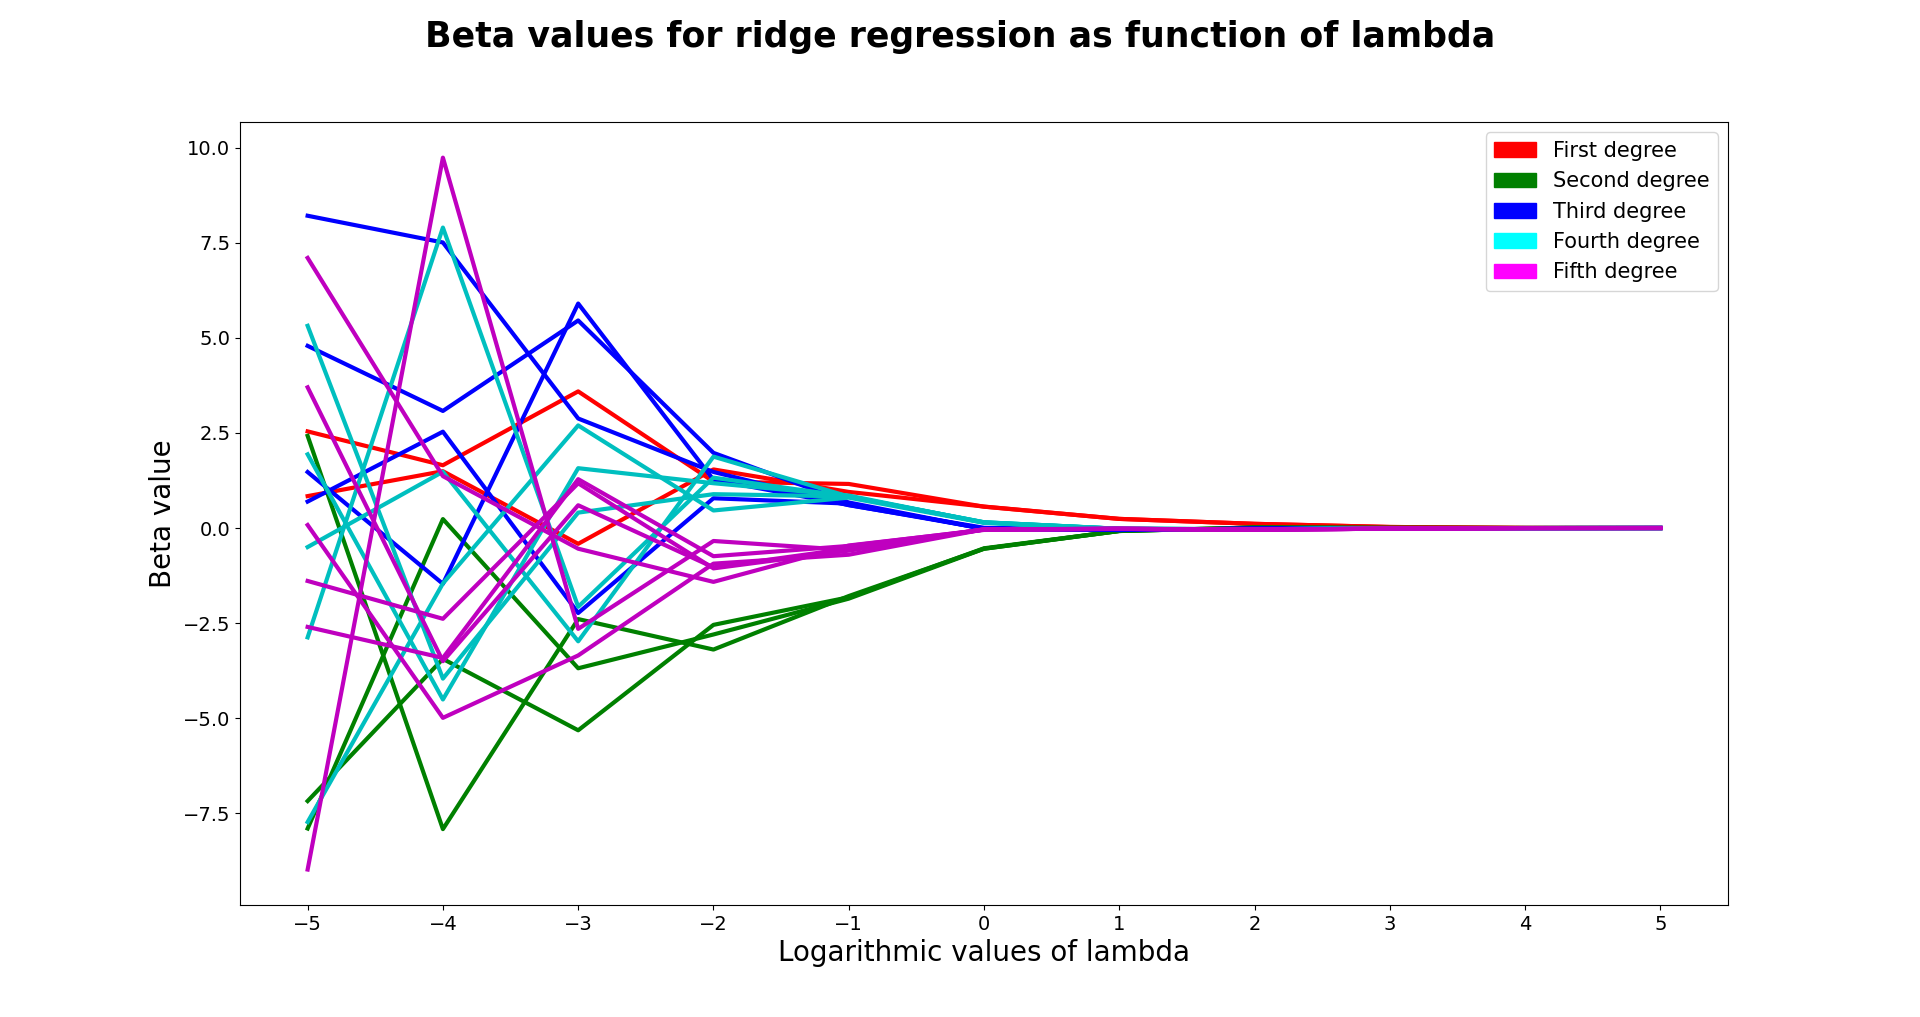
\includegraphics[width = 1\linewidth]{C:/Users/Sander/Documents/GitHub/FYS-STK4155/Project1/Report/Figures/LambdaPlot_n100_p5_noise0001_CV5_RIDGE.PNG}
\caption{\label{fig:LambdaPlotCV2} Regression coefficient values of up to $p = 5$ as function of logarithmic $\lambda$-value using the 5-fold CV method. The original dataset is of size 100. Here we have sorted polynomials of the same degree into the same color.}
\end{figure}

\begin{figure}[H]
\centering
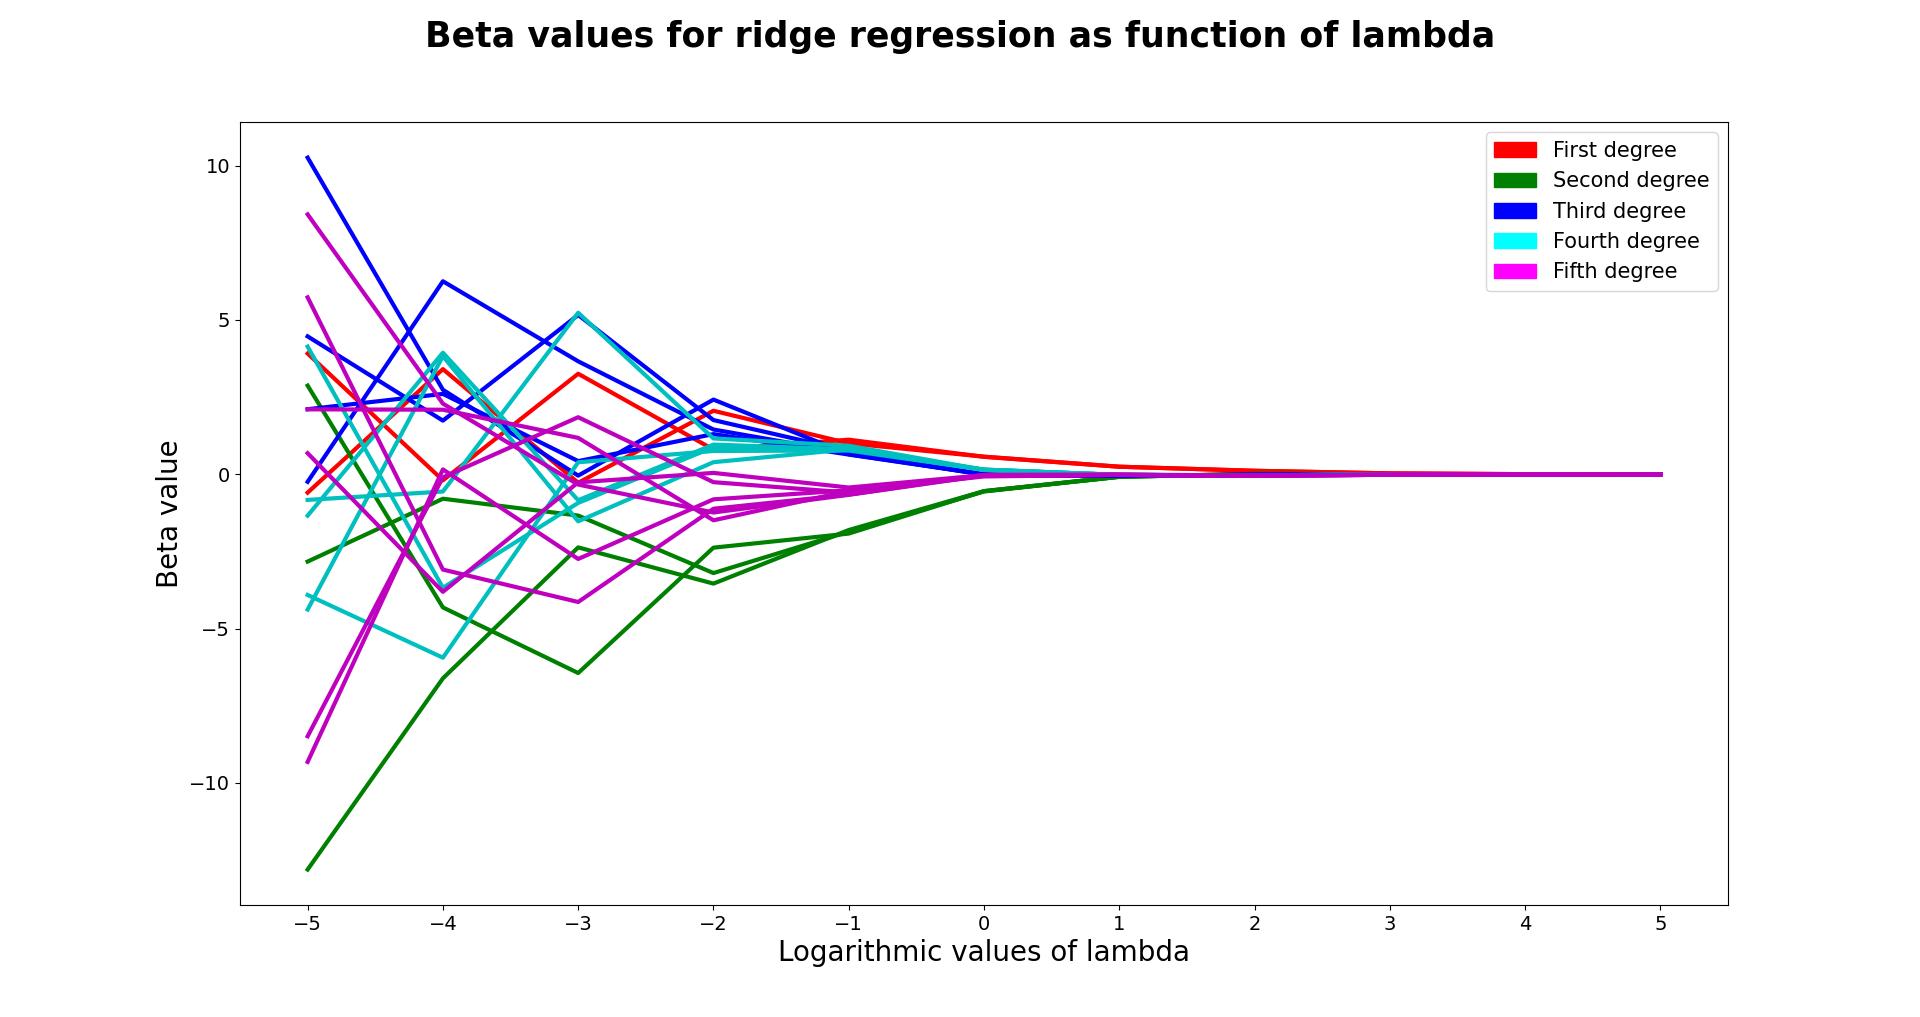
\includegraphics[width = 1\linewidth]{C:/Users/Sander/Documents/GitHub/FYS-STK4155/Project1/Report/Figures/LambdaPlot_n100_p5_noise0001_CV1_RIDGE.PNG}
\caption{\label{fig:LambdaPlotCV3} Regression coefficient values of up to $p = 5$ as function of logarithmic $\lambda$-value using the LOOCV method. The original dataset is of size 100. Here we have sorted polynomials of the same degree into the same color}
\end{figure}

\noindent One can observe that the regression coefficients all approach zero at about the same rate for all fold sizes. If we compared figures \ref{fig:LambdaPlotCV1}, \ref{fig:LambdaPlotCV2} and \ref{fig:LambdaPlotCV3} to figures \ref{fig:LambdaPlot2}, we observe that the regression coefficient values are higher for the CV resampling method. However, this is meaningless as it is when the coefficients approach zero that matters. With that, we again compare the figures and see that the Ridge regression reduces variables towards zero quicker when we use the CV resampling method, rather than the bootstrap method.
\\
With the information we have gathered so far, we can safely say that the Ridge regression impact the CV resampling method more than the bootstrap resampling method. However, the CV resampling method is more sensitive to different values of $\lambda$ than the bootstrap. 

\newpage

\noindent \textbf{e)} We now investigate the second shrinkage method, namely the Lasso regression. Like the Ridge regression, the Lasso shrinks the least significant variables, but the variables are set to exactly zero and not just close to zero. We can write the Lasso regression equation to be the same as the OLS equation (equation \ref{eq:LinReg}), but with an added penalty term to both sides 

\begin{equation}\label{eq:LassoDerive}
\begin{aligned}
\boldsymbol{\hat{y}}_{Lasso} + \lambda |\boldsymbol{\beta}|_1 = \textbf{X}\boldsymbol{\beta} + \lambda  |\boldsymbol{\beta}|_1
\end{aligned}
\end{equation}

\noindent where $|\boldsymbol{\beta}|_1$ is the L1 regularization. Solving equation \ref{eq:LassoDerive} for the regression coefficients in order to minimize the residual sum of squared yields

\begin{equation}\label{eq:LassoDerive2}
\begin{aligned}
some eq
\end{aligned}
\end{equation}

\noindent We can then perform the exact same investigation as done in exercise d, where we first plot the MSE as function of model complexity and the regression coefficients as function of $\lambda$ for the bootstrap resampling method as well as for 10-fold, 5-fold and leave-one-out cross-validations. The MSE plots are shown in figures \ref{fig:MSELasso1}, \ref{fig:MSELasso2}, \ref{fig:MSELasso3} and \ref{fig:MSELasso4}

\begin{figure}[H]
\centering
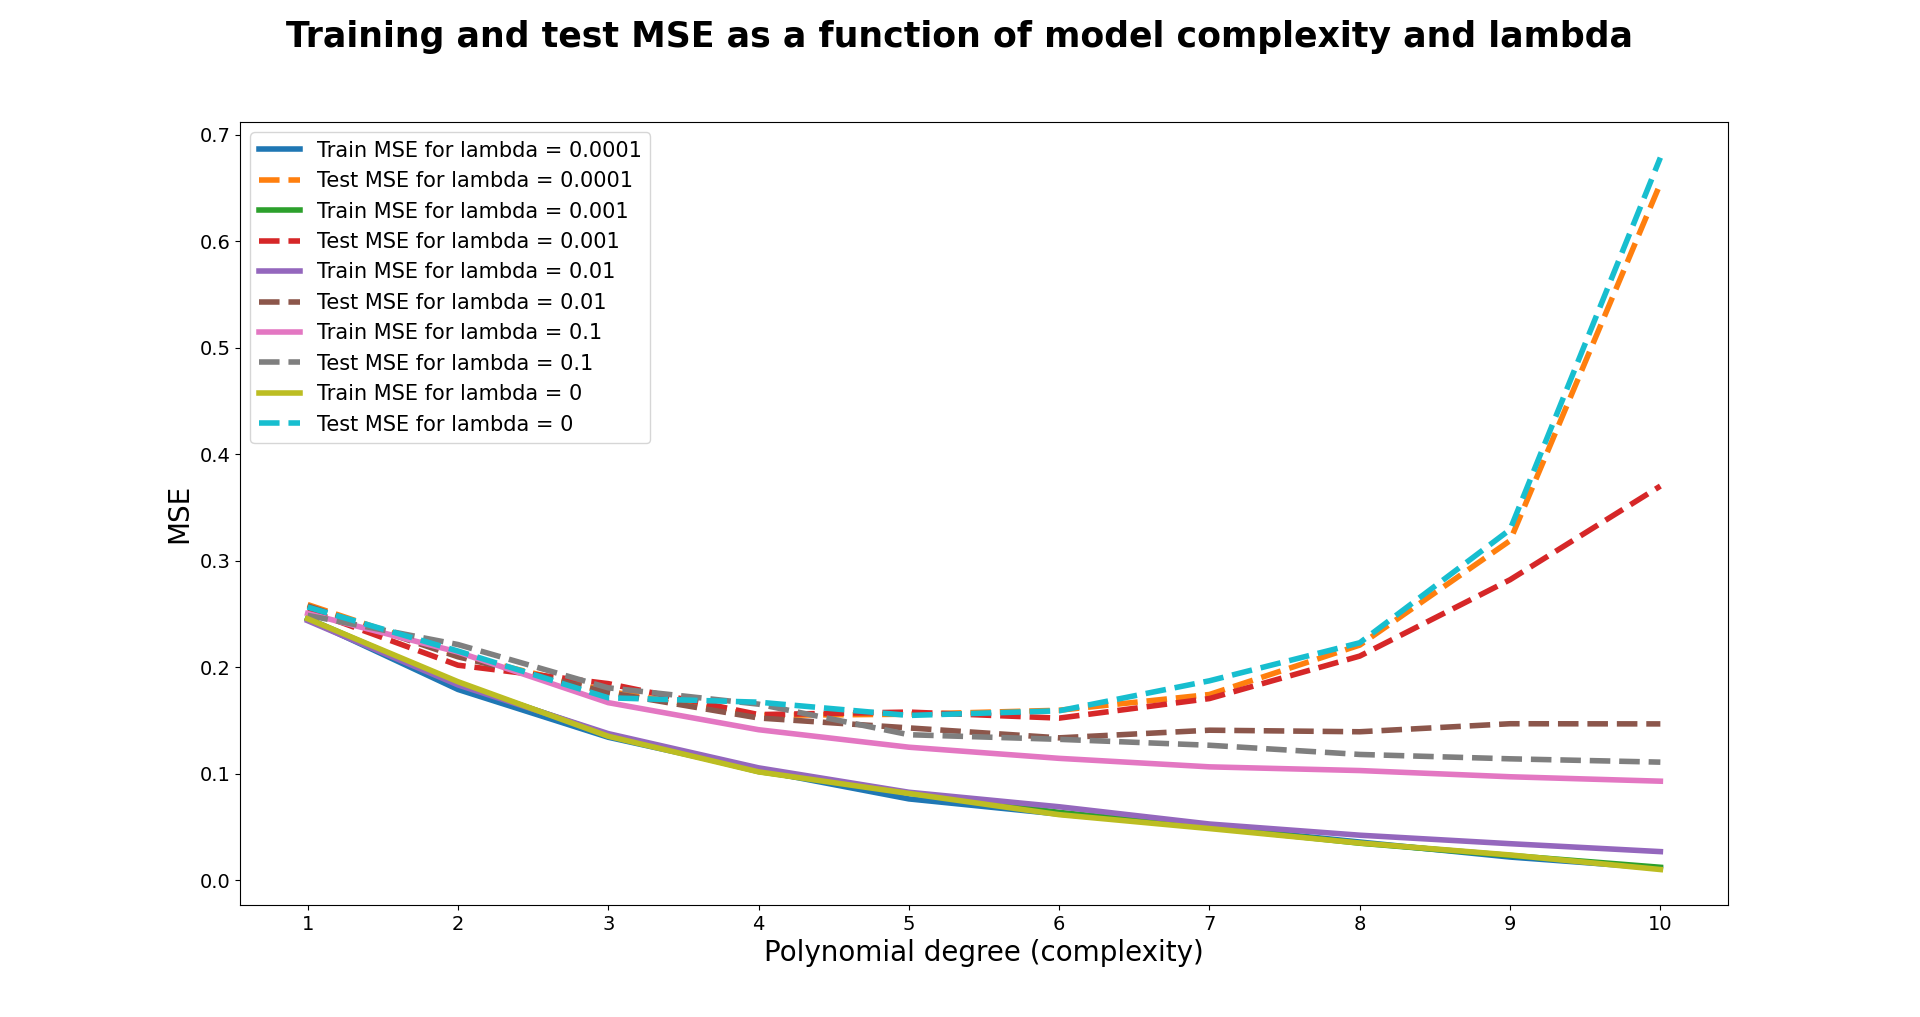
\includegraphics[width = 1\linewidth]{C:/Users/Sander/Documents/GitHub/FYS-STK4155/Project1/Report/Figures/MSEBOOT_n100_p10_noise0001_ts025_B100_Lasso.PNG}
\caption{\label{fig:MSELasso1} MSE as a function of polynomial degree up to 10 for different values of $\lambda$ using the bootstrap resampling method and a Lasso regression scheme. Here we have $100 \times 100$ observations randomly drawn from the original data with a noise level of $0.001$.}
\end{figure}

\begin{figure}[H]
\centering
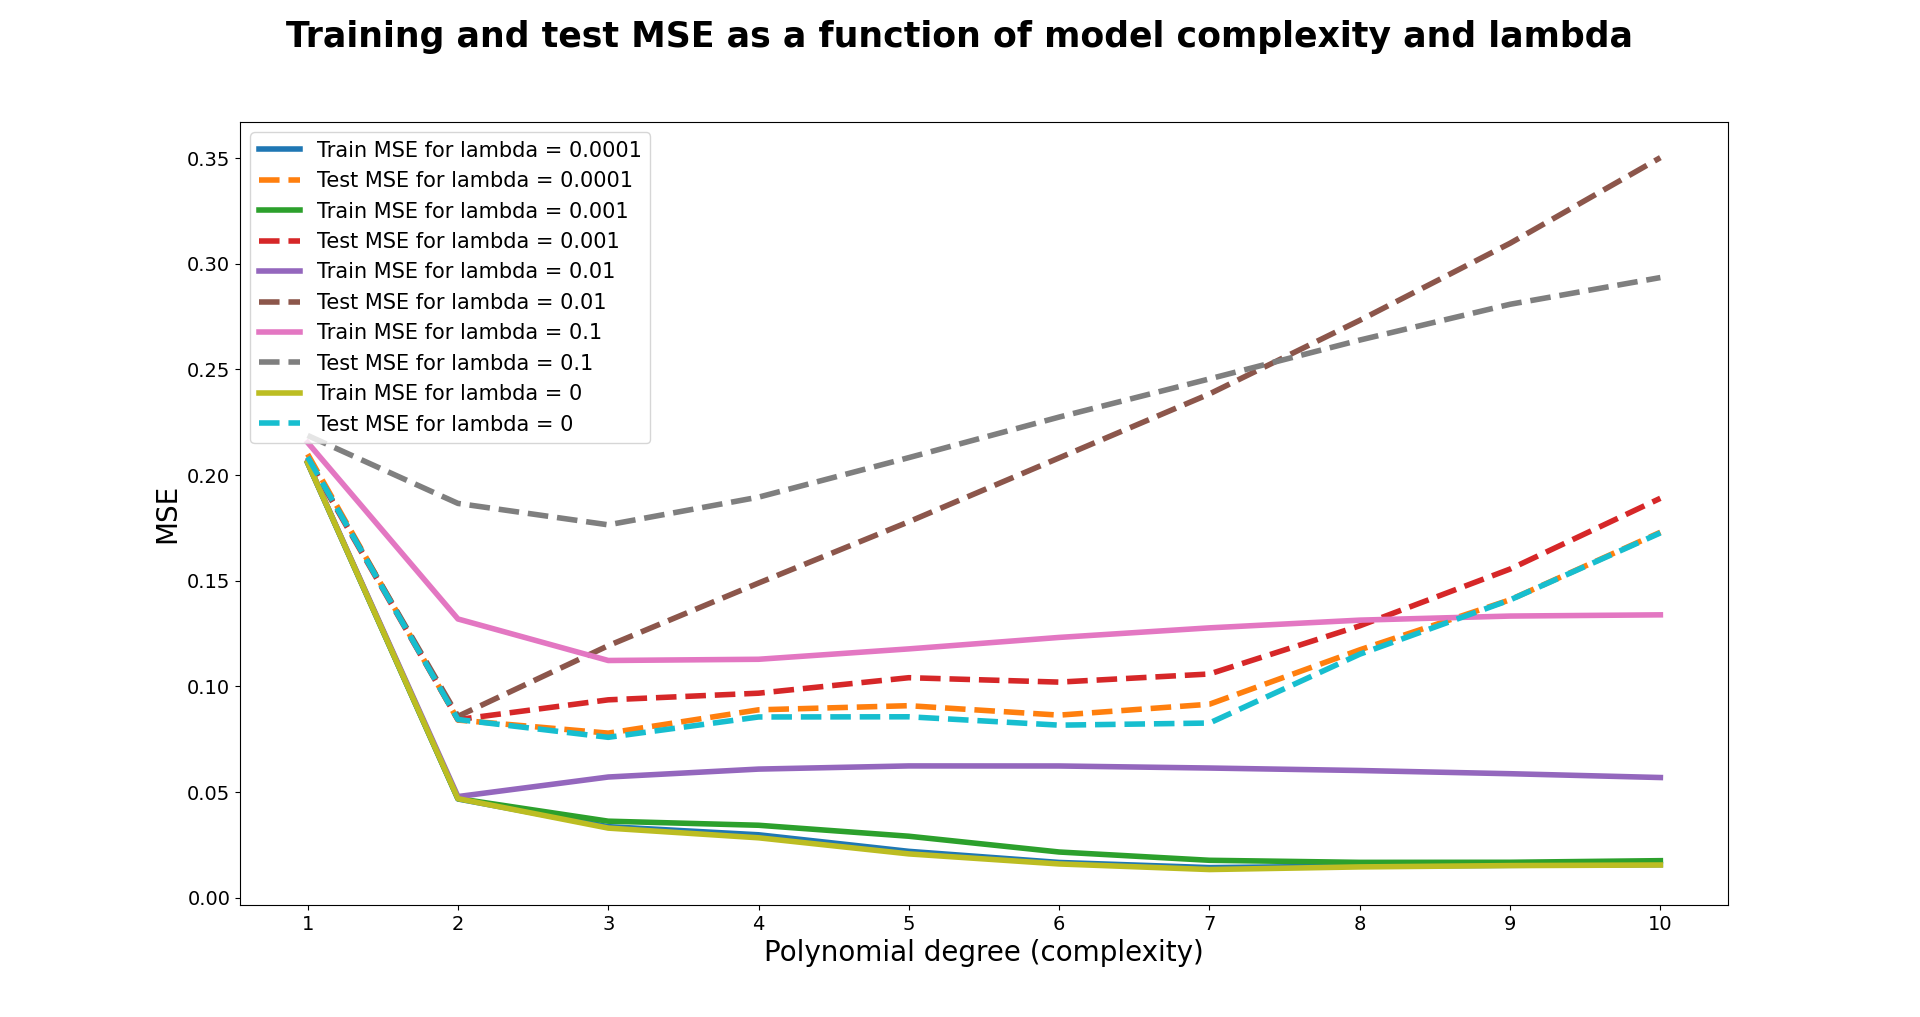
\includegraphics[width = 1\linewidth]{C:/Users/Sander/Documents/GitHub/FYS-STK4155/Project1/Report/Figures/MSECV_n100_p10_noise0001_CV10_Lasso.PNG}
\caption{\label{fig:MSELasso2} MSE as a function of polynomial degree up to 10 for different values of $\lambda$ using the 10-fold CV resampling method and a Lasso regression scheme. Here we have 100 observations while we consider every possible permutation of a 10-fold cross-validation with a noise level of $0.001$.}
\end{figure}

\begin{figure}[H]
\centering
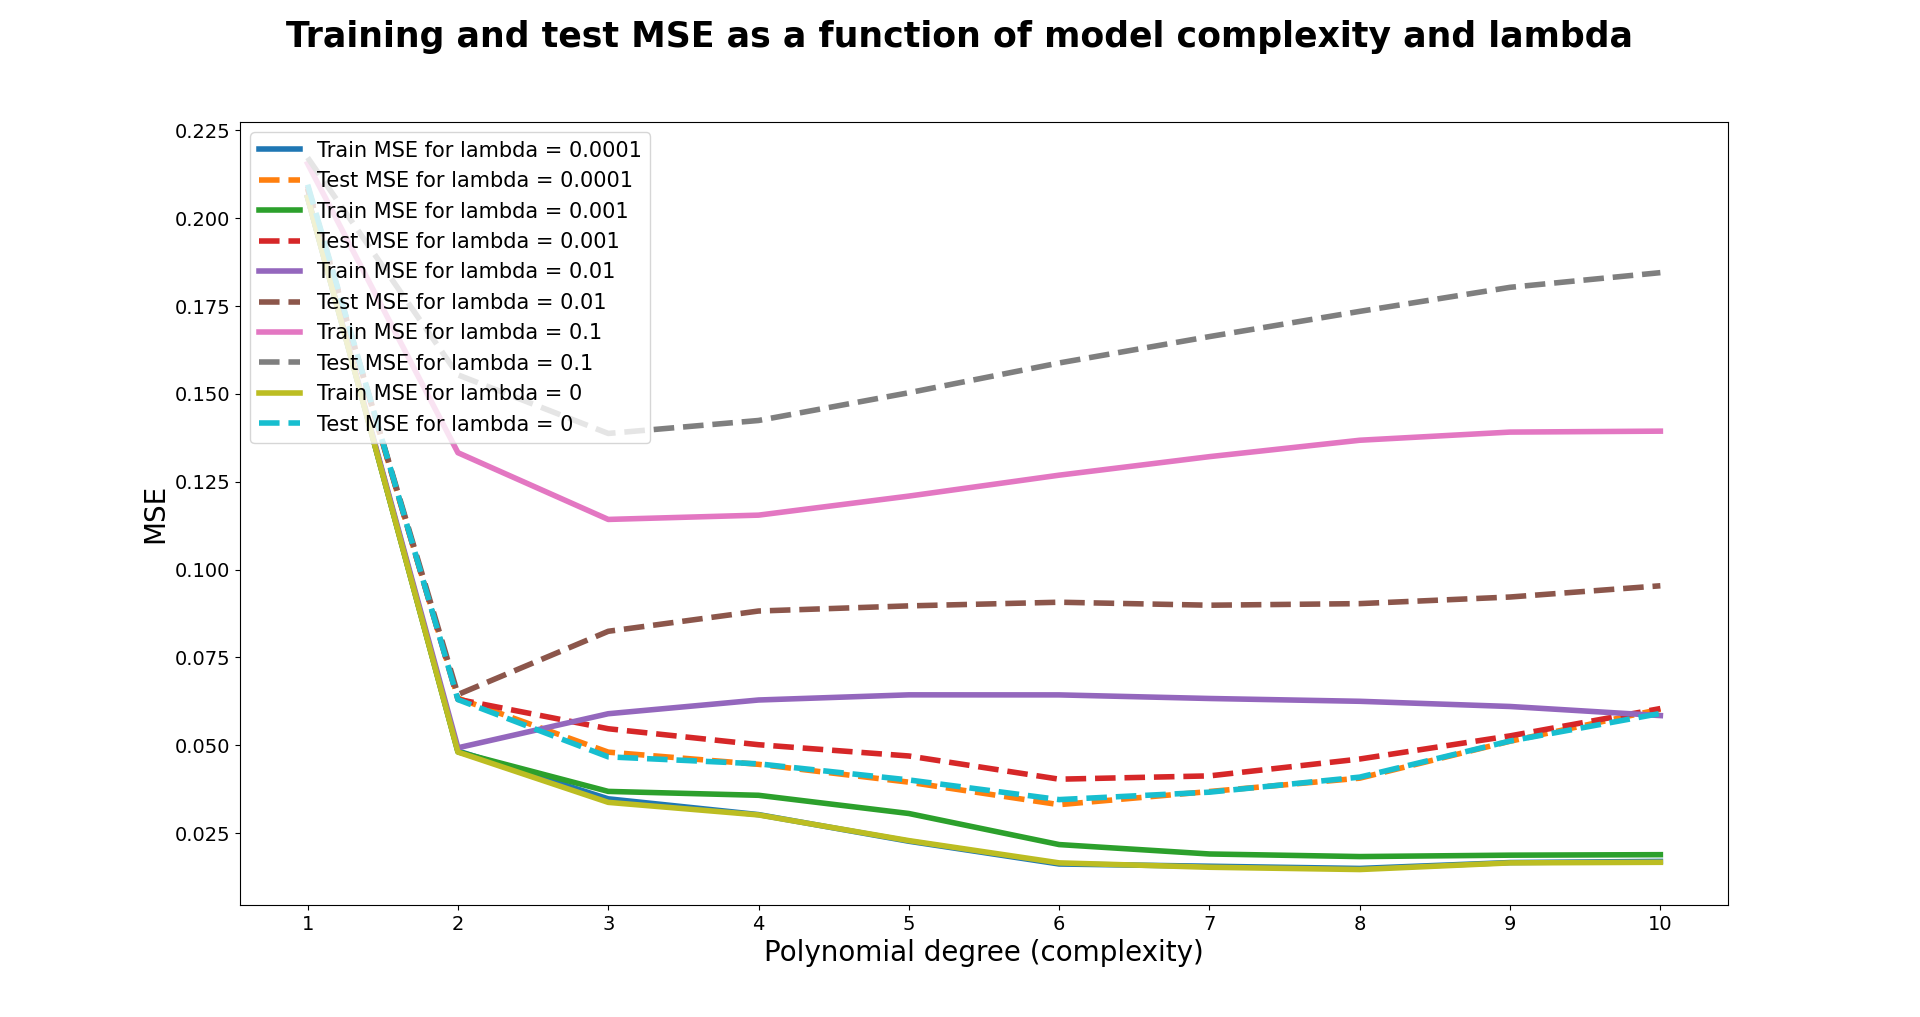
\includegraphics[width = 1\linewidth]{C:/Users/Sander/Documents/GitHub/FYS-STK4155/Project1/Report/Figures/MSECV_n100_p10_noise0001_CV5_Lasso.PNG}
\caption{\label{fig:MSELasso3} MSE as a function of polynomial degree up to 10 for different values of $\lambda$ using the 5-fold CV resampling method and a Lasso regression scheme. Here we have 100 observations while we consider every possible permutation of a 5-fold cross-validation with a noise level of $0.001$.}
\end{figure}

\begin{figure}[H]
\centering
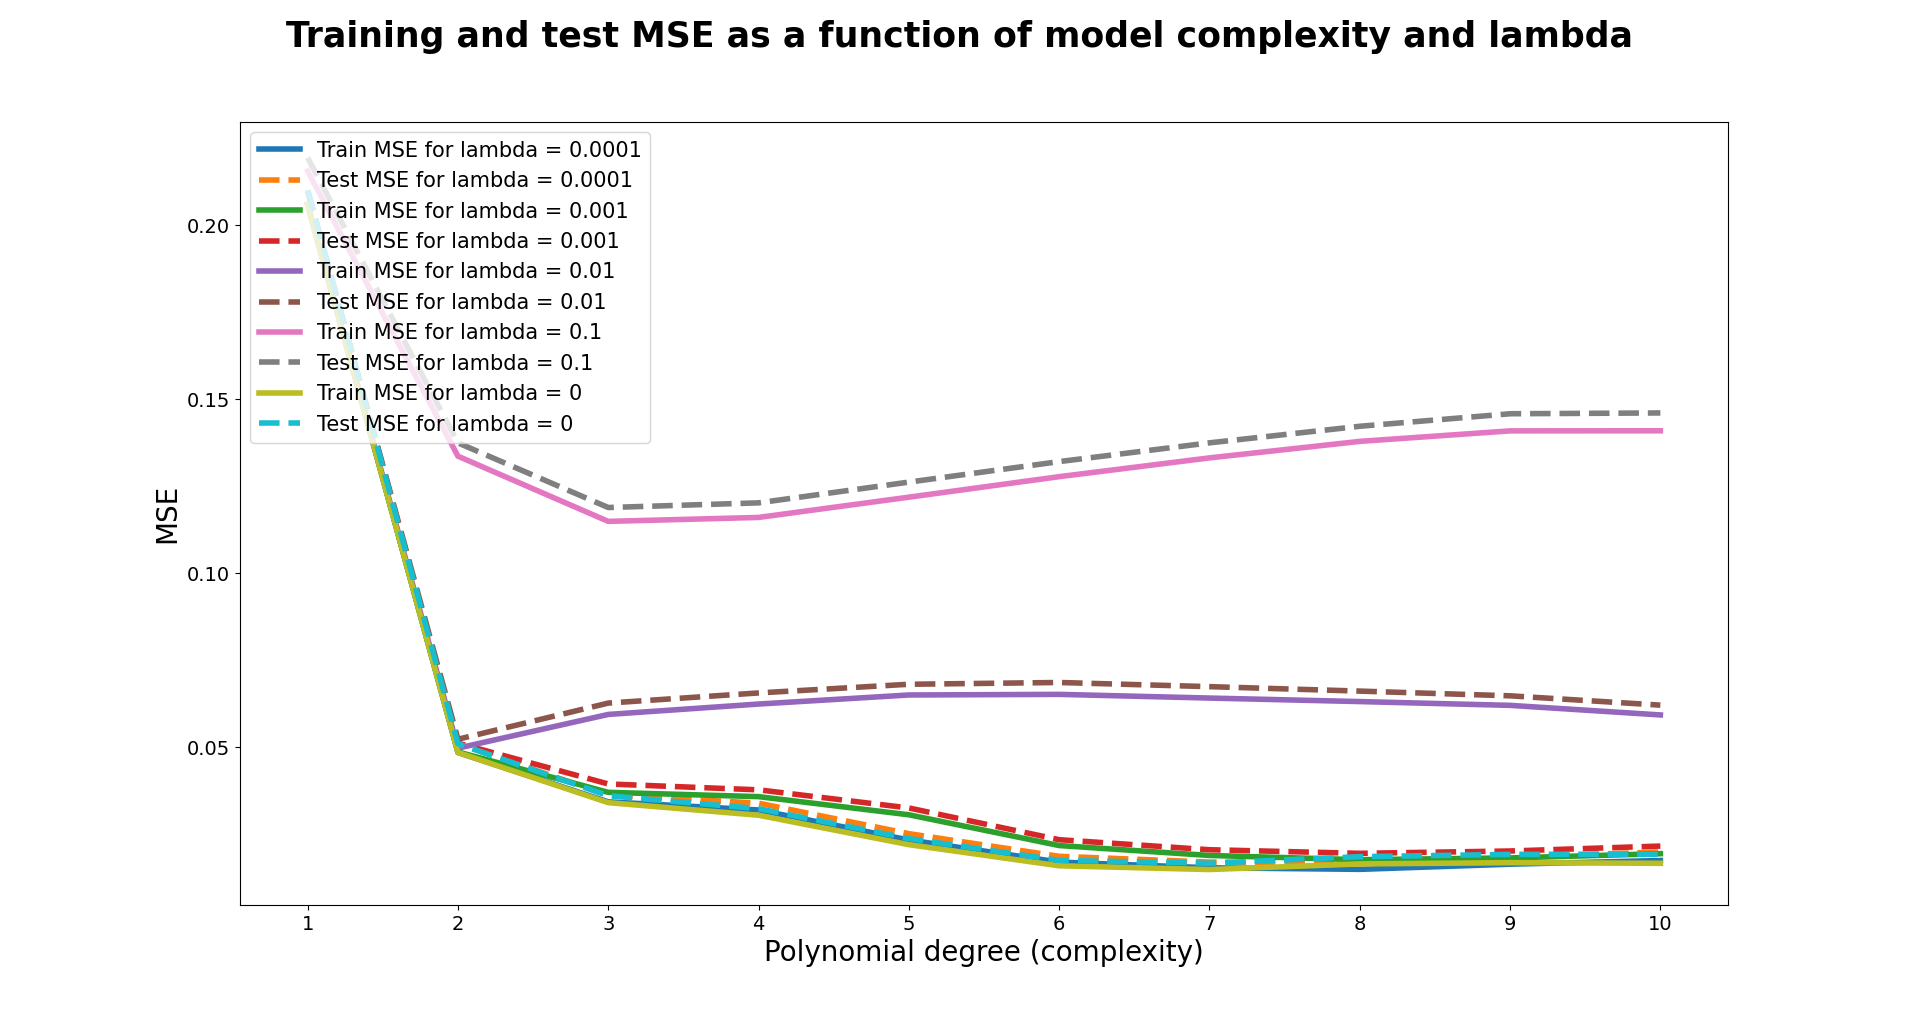
\includegraphics[width = 1\linewidth]{C:/Users/Sander/Documents/GitHub/FYS-STK4155/Project1/Report/Figures/MSECV_n100_p10_noise0001_CV1_Lasso.PNG}
\caption{\label{fig:MSELasso4} MSE as a function of polynomial degree up to 10 for different values of $\lambda$ using the LOOCV resampling method and a Lasso regression scheme. Here we have 100 observations while we consider every possible permutation of a LOOCV with a noise level of $0.001$.}
\end{figure}

\noindent Let us first discuss the difference between the bootstrap resampling method seen in figure \ref{fig:MSELasso1} and the CV resampling method seen in figures \ref{fig:MSELasso2}, \ref{fig:MSELasso3} and \ref{fig:MSELasso4}. The models creating using bootstrap seem much smoother than the models using CV. More importantly, we observe that the bootstrap models tend to increase their MSE exponentially, while the CV models tend to increase their MSE linearly. This may be important if one wishes to create a model of a high degree without letting the MSE get out of hand. 
\\
As for the dependence on different $\lambda$-values, we can observe the same effect as in exercise d in figures \ref{fig:MSERidgeCV1}, \ref{fig:MSERidgeCV2} and \ref{fig:MSERidgeCV3}, namely that increasing the value of $\lambda$ increases the overall MSE. There seem to be one exception however as the model using $\lambda = 0$ had relatively low MSE. This is because this particular model is equivalent to the OLS model and will therefore perform better than some incremental value just under zero. 
\\
Another observations is that some models using low values of $\lambda$ never really increase in MSE. This is particularly the case for the bootstrap and LOOCV models where polynomials of degree 10 have less $0.1$ in MSE. Such a feet is possible due to the variable shrinkage done by the Lasso regression scheme. Removing variables makes the model less prone to over-fitting, thus reducing the MSE at higher complexity. This means that using models with a high number of bootstrap iterations or low number of folds while using low values of $\lambda$ allows us to create a model for higher order polynomials, which in turn may increase the models predictive capabilities.
\\
Let us now study how the regression coefficients change as a function of $\lambda$ as we already suspect that some of them have been set to zero by the Lasso regression scheme. Figure \ref{fig:LambdaLasso1}, \ref{fig:LambdaLasso2}, \ref{fig:LambdaLasso3} and \ref{fig:LambdaLasso4} show how regression coefficients behave as function of $\lambda$

\begin{figure}[H]
\centering
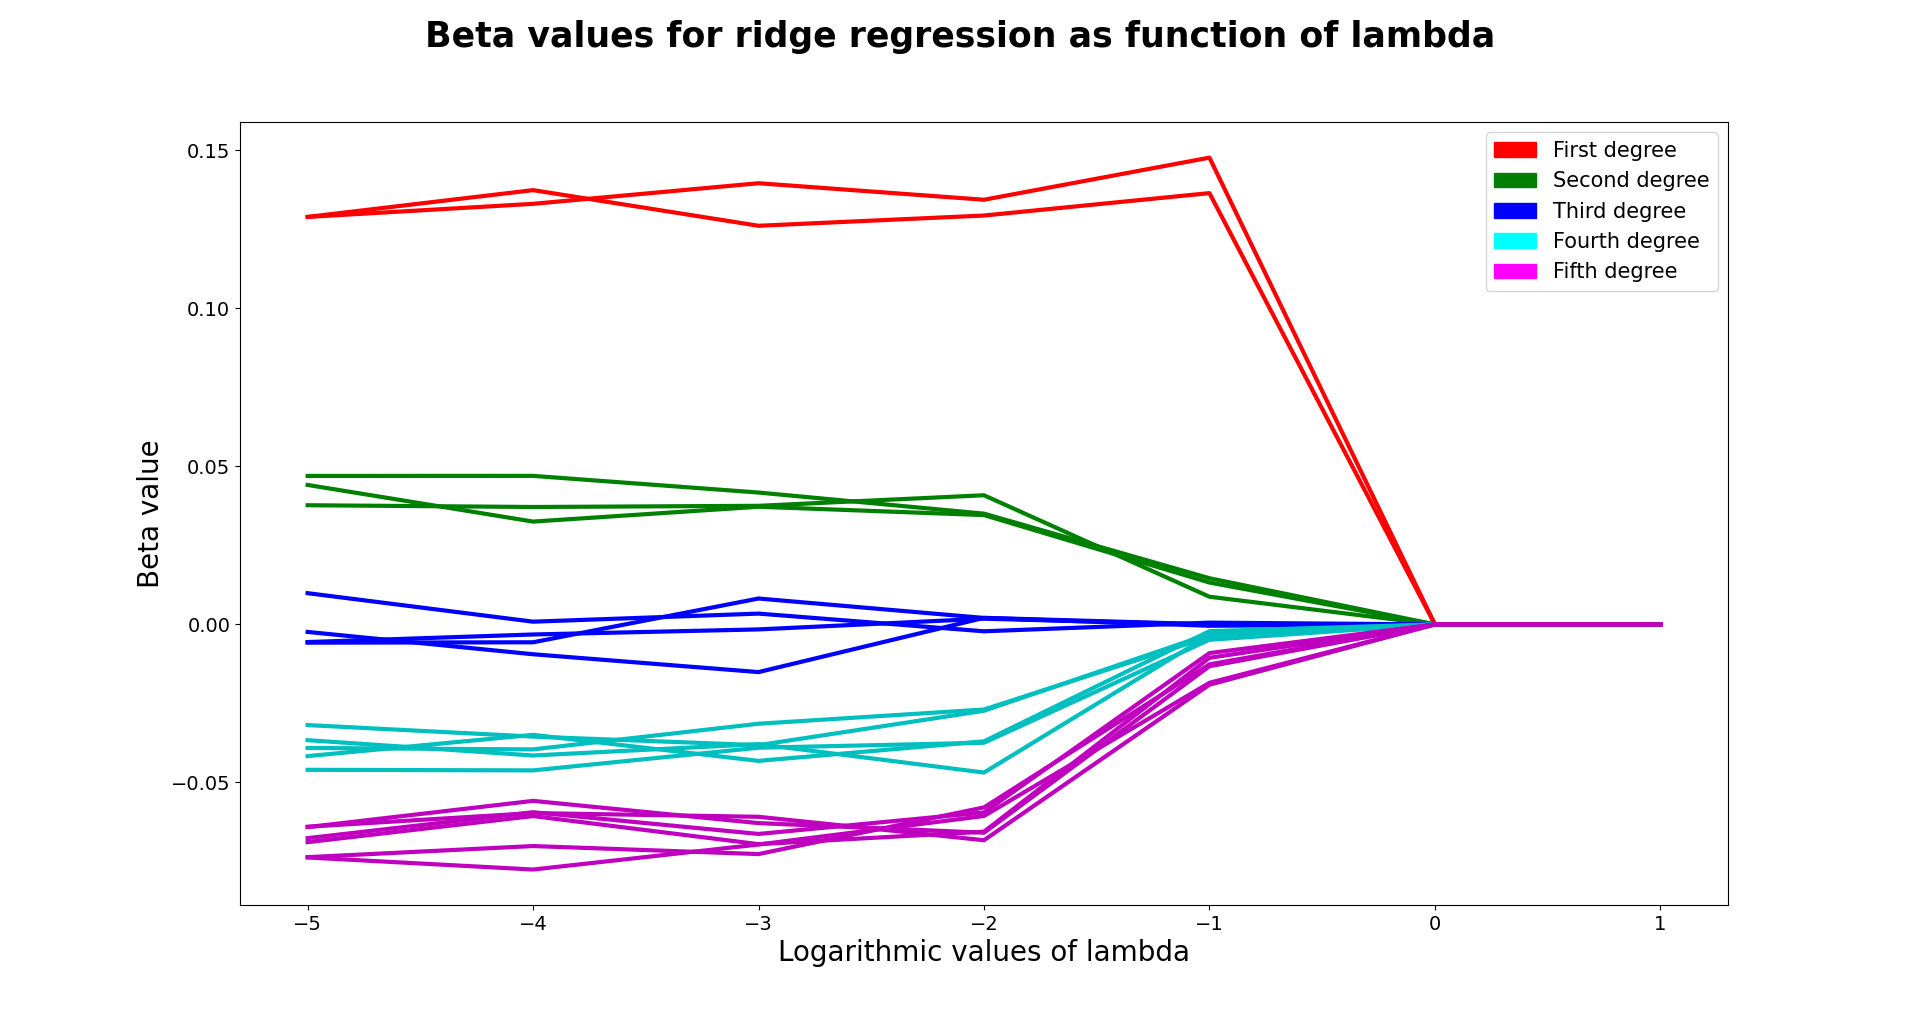
\includegraphics[width = 1\linewidth]{C:/Users/Sander/Documents/GitHub/FYS-STK4155/Project1/Report/Figures/LambdaPlot_n100_p5_noise0001_ts025_B100_LassoSort.PNG}
\caption{\label{fig:LambdaLasso1} Regression coefficient values of up to $p = 5$ as function of logarithmic $\lambda$-value using the bootstrap resampling method. The original dataset is of size 100 with a noise-level of $0.001$. Here we have sorted polynomials of the same degree into the same color.}
\end{figure}

\begin{figure}[H]
\centering
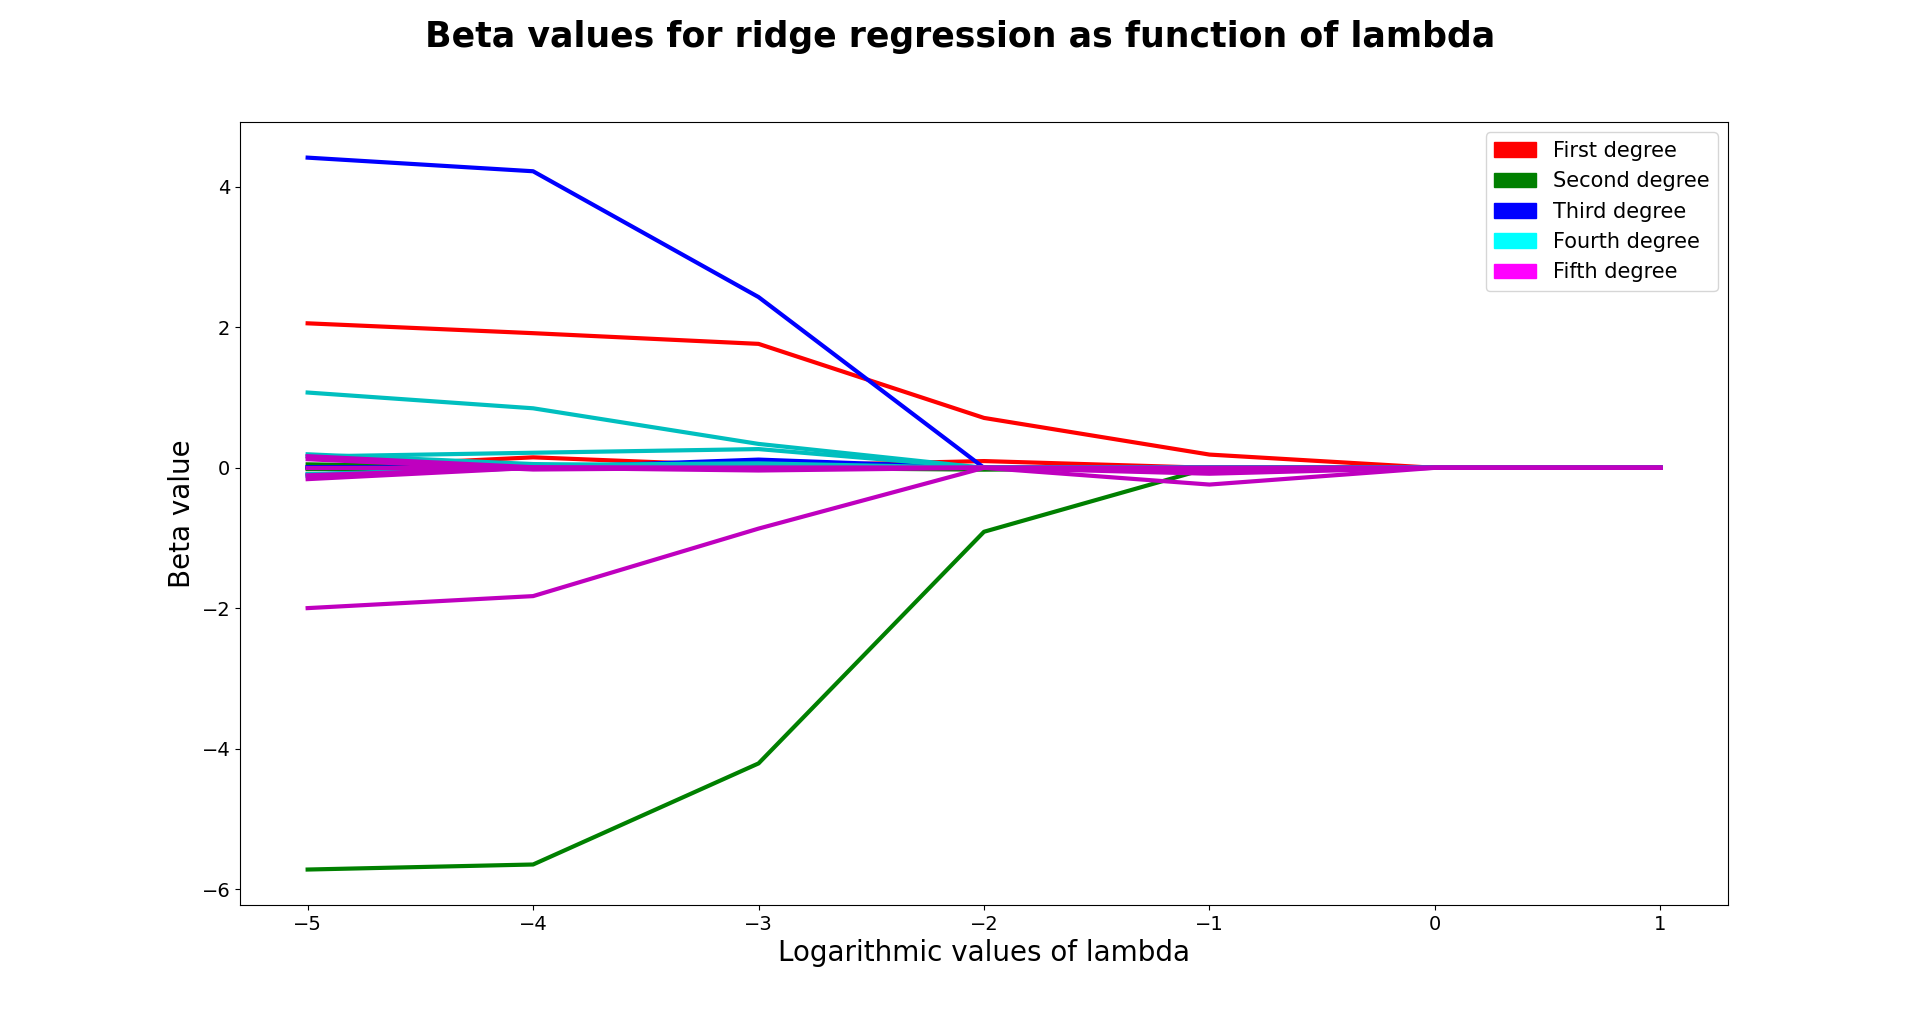
\includegraphics[width = 1\linewidth]{C:/Users/Sander/Documents/GitHub/FYS-STK4155/Project1/Report/Figures/LambdaPlot_n100_p5_noise0001_CV10_LassoSort.PNG}
\caption{\label{fig:LambdaLasso2} Regression coefficient values of up to $p = 5$ as function of logarithmic $\lambda$-value using the 10-fold CV resampling method. The original dataset is of size 100 with a noise-level of $0.001$. Here we have sorted polynomials of the same degree into the same color.}
\end{figure}

\begin{figure}[H]
\centering
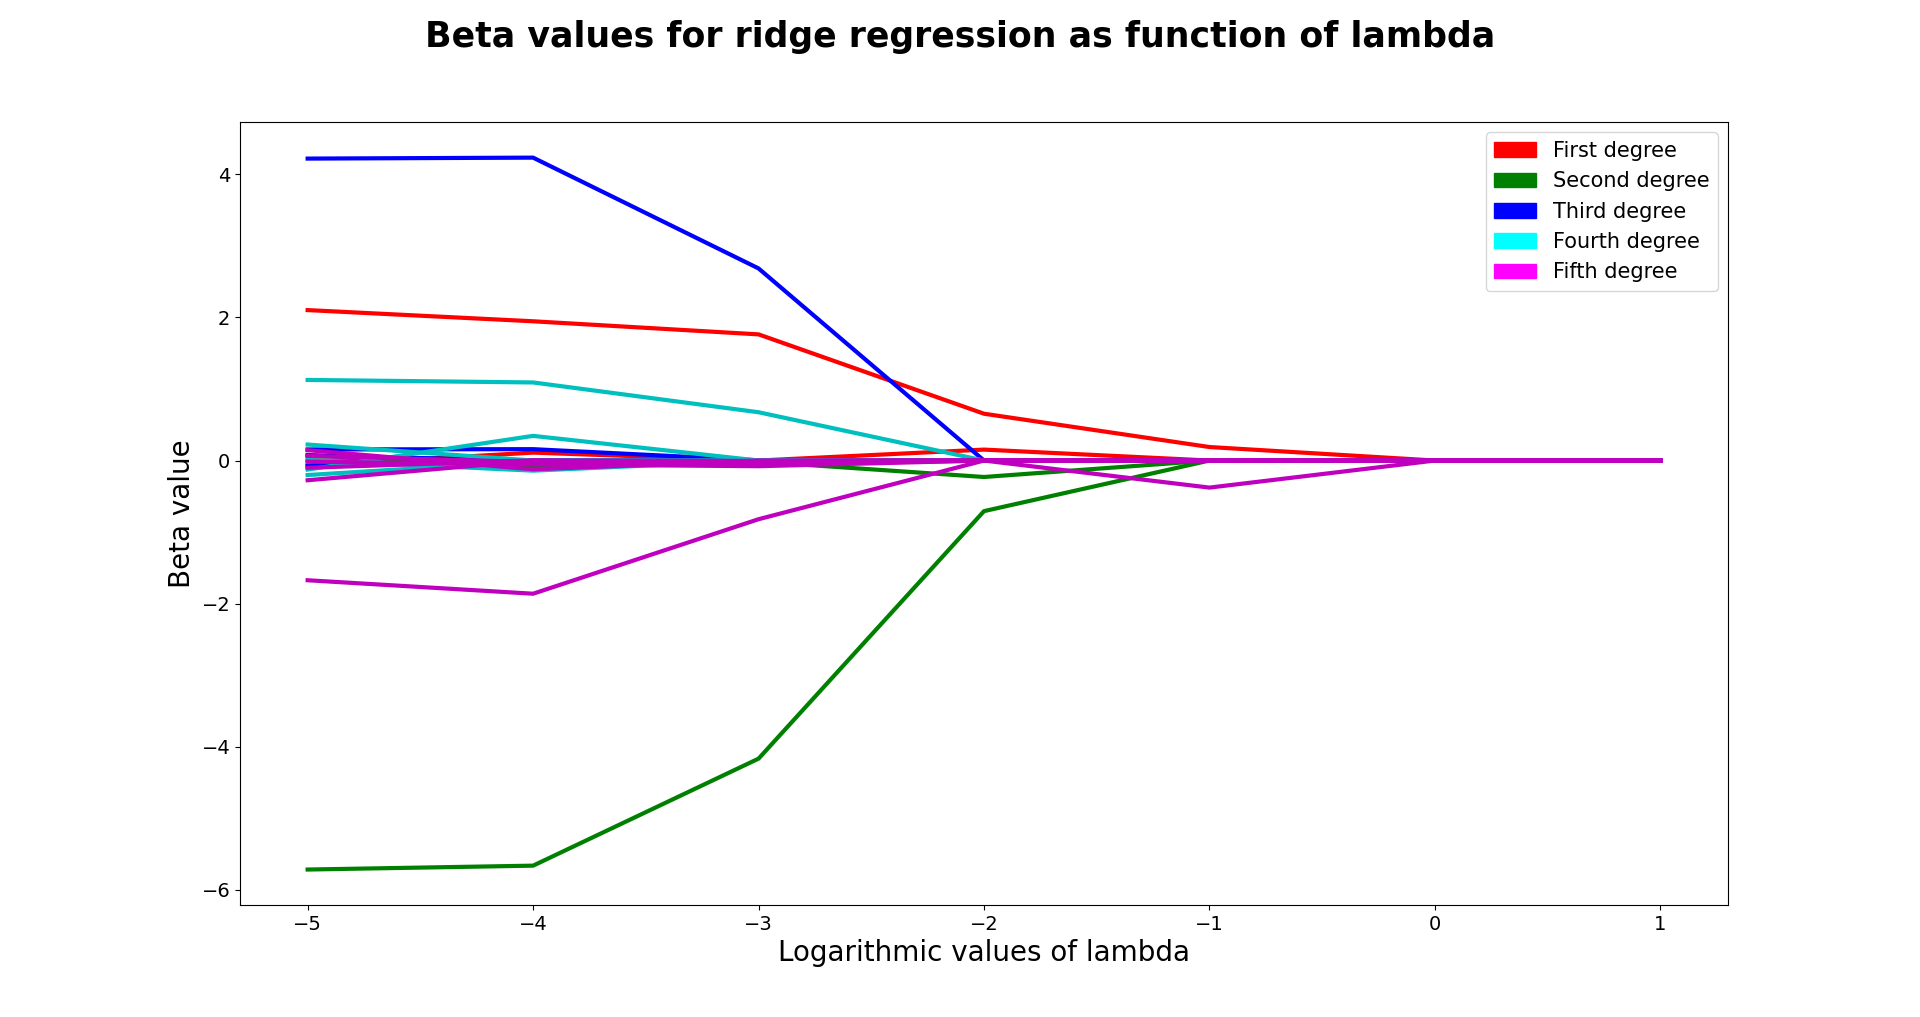
\includegraphics[width = 1\linewidth]{C:/Users/Sander/Documents/GitHub/FYS-STK4155/Project1/Report/Figures/LambdaPlot_n100_p5_noise0001_CV5_LassoSort.PNG}
\caption{\label{fig:LambdaLasso3} Regression coefficient values of up to $p = 5$ as function of logarithmic $\lambda$-value using the 5-fold CV resampling method. The original dataset is of size 100 with a noise-level of $0.001$. Here we have sorted polynomials of the same degree into the same color.}
\end{figure}

\begin{figure}[H]
\centering
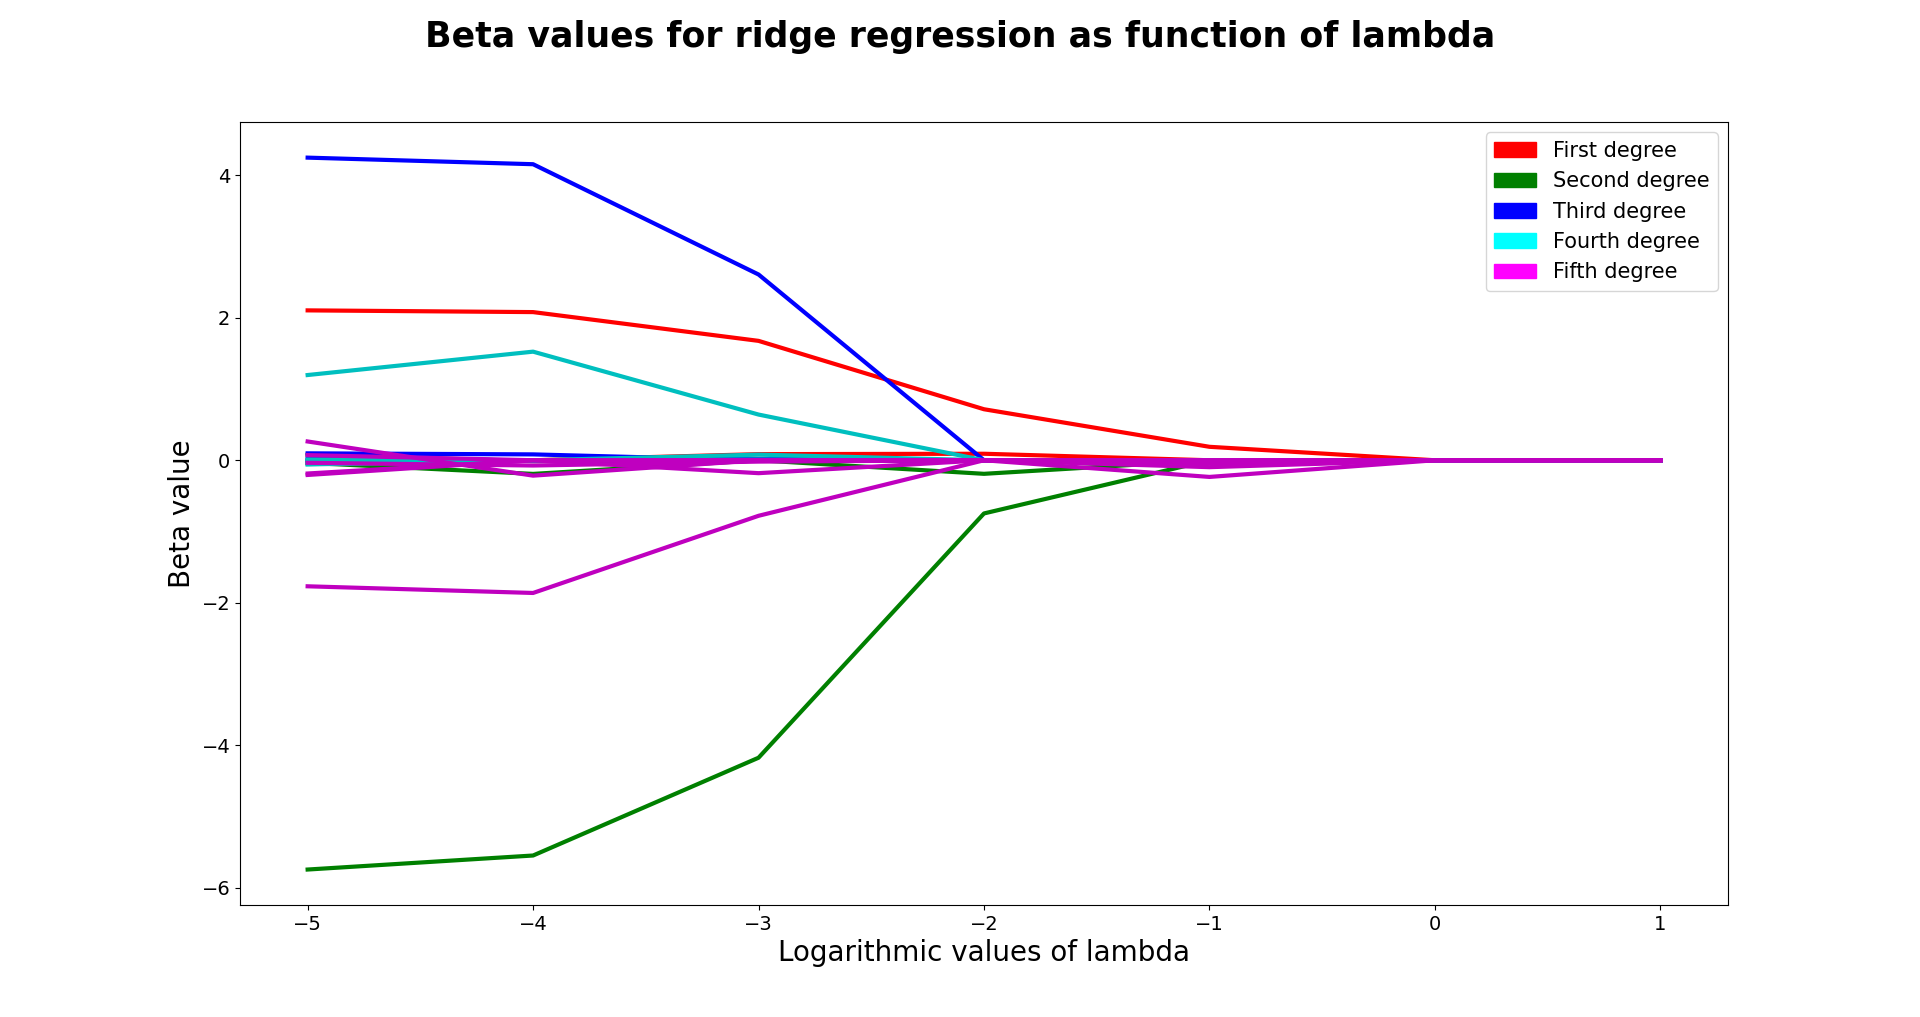
\includegraphics[width = 1\linewidth]{C:/Users/Sander/Documents/GitHub/FYS-STK4155/Project1/Report/Figures/LambdaPlot_n100_p5_noise0001_CV1_LassoSort.PNG}
\caption{\label{fig:LambdaLasso4} Regression coefficient values of up to $p = 5$ as function of logarithmic $\lambda$-value using the LOOCV resampling method. The original dataset is of size 100 with a noise-level of $0.001$. Here we have sorted polynomials of the same degree into the same color.}
\end{figure}

\noindent Comparing the above plots really shows the difference in how the bootstrap and CV resampling methods behave with respect to their models regression coefficients. We can observe that both methods shrink the variables to zero, but at different values of $\lambda$. The CV methods (which all seem to be equivalent) reduce some MOREMOREMOREMORE
\\
We also notice that the Lasso regression reduces the variables at lower values of $\lambda$ than the Ridge regression (figures \ref{fig:LambdaPlot2}, \ref{fig:LambdaPlotCV1}, \ref{fig:LambdaPlotCV2} and \ref{fig:LambdaPlotCV3}). This is typical as the $L_1$ norm used in the Lasso regression is more sensitive to the shrinkage parameter $\lambda$ than the $\L_2$ norm. 

\newpage

\noindent \textbf{f)} In this exercise we prepare the terrain data set called "SRTM\textunderscore data\textunderscore Norway\textunderscore 1" which is data collected from Norway. This data was chosen as we had trouble registering an account on the webpage \href{{https://earthexplorer.usgs.gov/}}{\nolinkurl{https://earthexplorer.usgs.gov/}}, so we settled for the given data set on the FYS-STK4155 github page. The terrain data is loaded into python and the following image is obtained

\begin{figure}[H]
\centering
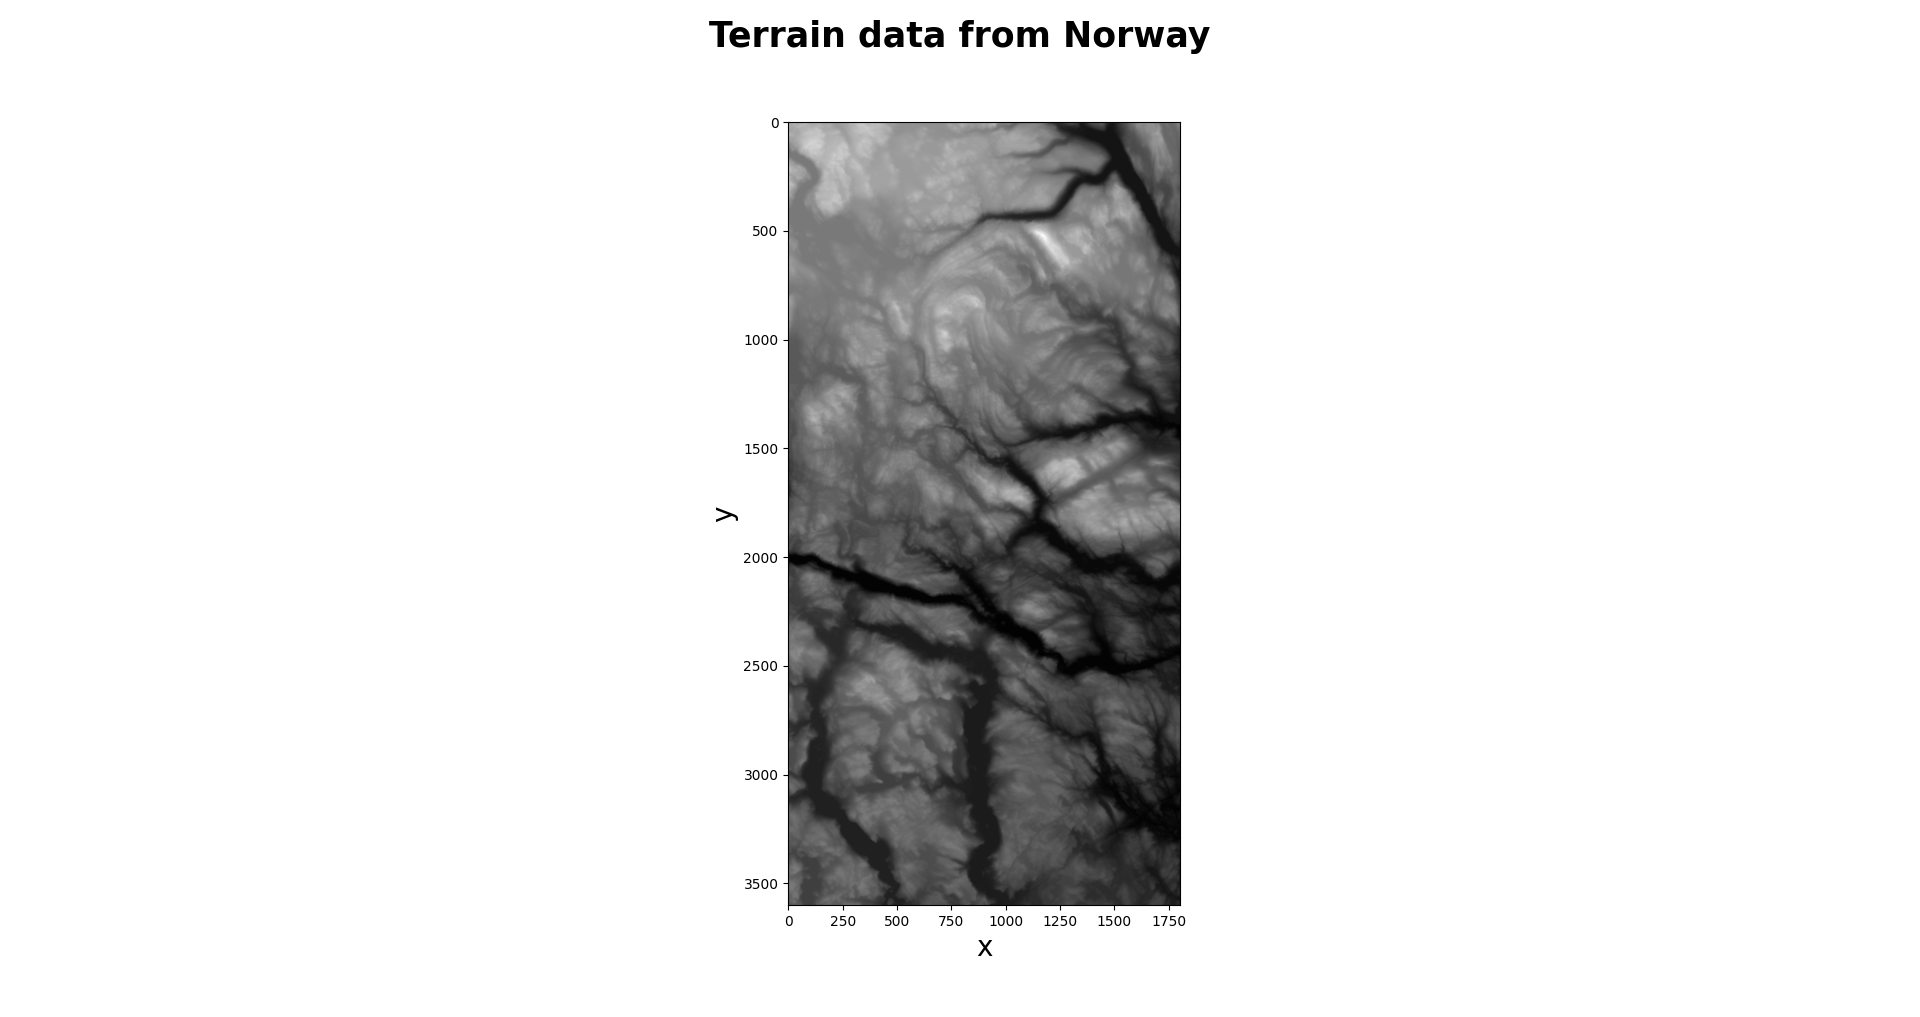
\includegraphics[width = 1\linewidth]{C:/Users/Sander/Documents/GitHub/FYS-STK4155/Project1/Report/Figures/terrainData2.PNG}
\caption{\label{fig:terrainData1} Terrain data over Norway.}
\end{figure}

\noindent This data will from now act as the response $\hat{y}$ just like the Franke function have been used so far. Since we now have already developed the tools to model the image in figure \ref{fig:terrainData1}, we can proceed to exercise g.

\newpage

\noindent \textbf{g)} a

\newpage

\begin{center}
\Large{\textbf{References}}
\end{center}

\begin{itemize}
  \item Reference
\end{itemize}

\end{document}
